% Chapter 4: coming along nicely. Be concise

\chapter{Data and methods} % Write in your own chapter title
\label{Chapter4}
% \lhead{Chapter 4. \emph{Data and methods}} % Write in your own chapter title
\fancyhead[RO,LE]{Chapter 4. Data and methods} %2side
\fancyhead[RE,LO]{\thepage}
\section{Introduction} 
% this thesis is a data-driven exploration of the energy costs of commuting.
To fully describe and understand the energy used in travel to work, a large
amount of data is needed. Behavioural, technical, infrastructural and even
economic data would be required at a high level of spatial and temporal
resolution over a wide area and a long timespan to provide a complete
picture of the flows within the transport-to-work energy system. %!!! Make this
The ideal dataset would also contain grid references of both the origin and
destination of every trip to and from work, the
route distance (which may change from one day to the next), the specifications
of the primary vehicle used and, ideally, measurement of the food or fuel
consumed as a result.

It is worth briefly considering what this giant dataset would look like: the
methods can be seen as an attempt to approximate a simplified version this
omniscient information source, through modelling. \Cref{fdata-ideal} illustrates
the numerous connections to additional datasets not traditionally included in
travel surveys that would be needed for the most detailed view.
The thought experiment led to the imaginary Comprehensive
Commuting-Energy Database (CCED). This main dataset would be part of a wider
`data schema' of connected tables \citep{Obe2011} as it would depend on
detailed additional
information about individuals, the vehicles they drive, up-to-date
information on where they live and work, as well as detailed information on
every single trip to work they make for an accurate assessment of energy costs
and the factors influencing them. To gain an understanding of the complexity of
this dataset, let us picture its size for the UK. Assume that 30 million people
are employed,\footnote{During
the 3$^{rd}$ quarter of 2012, there were 29.86 million
employed
people in the UK according to the
\href{http://www.ons.gov.uk/ons/dcp171778_292911.pdf}{Office for National
Statistics}}
making, on average, 200
home-work round trips per year. This would mean the CCED would need to contain
12 billion rows of data each year. Even ignoring the complexities added by the
linked datasets,\footnote{The CCED would need to link to the constantly changing
home-work
locations (currently untracked by the government, except during the census),
household composition, energy use data and vehicle ownership datasets. This
would require constant, probably automated monitoring and computer
infrastructure that is currently beyond most local authorities to store, analyse
and interpret. Large data management
organisations such as Google and Facebook have shown that such vast
`live' databases are possible, however. A state-controlled online
data-logging system, which harnesses near-total smart-phone penetration, could
conceivably move towards this vision. } keeping this dataset updated live would
be far beyond the government's current official data collection capabilities.
The largest microsimulation run performed for this research was of $\sim$2 million
commuters in Yorkshire and the Humber, over 3 orders of magnitude smaller that
the CCED for a single year. Given that the analysis was unwieldy, it seems such
a large dataset would pose major problems to current mainstream computer
hardware.

\begin{figure}
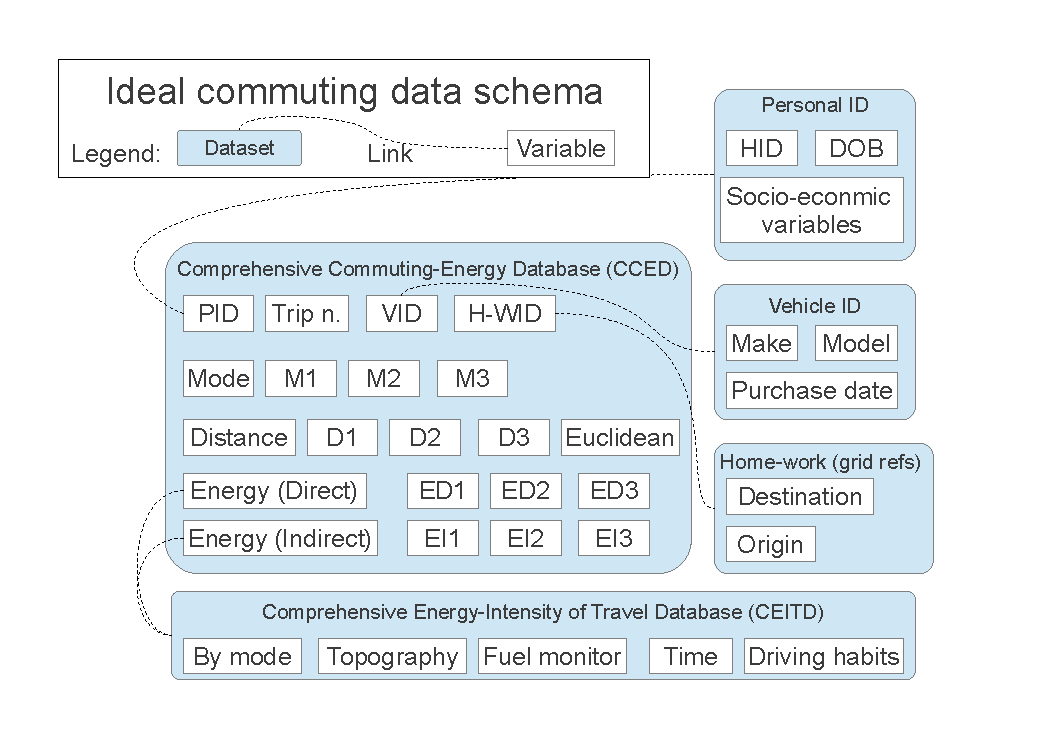
\includegraphics[width=14cm]{data-ideal}
\caption[Idealised data schema for studying energy use in commuting]{Idealised
data schema for studying energy use in commuting. The imaginary CCED database
would need to link to other, equally detailed datasets to work.}
\label{fdata-ideal}
\end{figure}

Of course, the available datasets do not match the detail of the imaginary CCED.
Budgets for data collection, confidentiality and technical
considerations combine with the practical
difficulties of monitoring the energy used by hundreds of thousands of unique
vehicles. Based on these difficulties, one could argue that the data
limitations are insurmountable and that more qualitative approaches are needed.
This research is based on the opposite view: that the inherent data limitations
mean that the datasets that \emph{are} available are
absolutely critical. Systematically collected data has a much better chance of
meeting the research aims, as set-out in \cref{s:aims} than purely qualitative
information. Without good statistics, one would have to resort to personal
observation and anecdote, sources that are unlikely to be
representative of the system as a whole \citep{Rubin1987}. Because the available
datasets cannot be
changed, whereas the methods used to analyse and model them can, the approach
taken here is \emph{data-driven} (as opposed to model driven)
\citep{anselin1989special}: the starting-point is the available data.
After the introduction, this chapter describes the input
datasets (\cref{senergyusedata} to \cref{sadditional}) and then
explains the methods used to process them and evaluate the outputs (\cref{setsim} to
\cref{smeval}). The final section explores methods for generating
integer results, which are useful in agent-based applications (\cref{s:integerisation}).

Due to its policy relevance, the methods 
are treated primarily as means rather than ends in themselves throughout
the majority of the thesis. In this chapter the emphasis reverses, and the methods
(and the datasets on which they depend) become the focus. It would be an
exaggeration to say that the data and
methods are seen here as ends in themselves, as they all contribute towards the
aims. Yet effort has been made to explain them in general terms. An
additional aim of this chapter is to illustrate clearly how the methods
were implemented, allowing others to replicate the results. It should also be
clear by the end of this chapter that the methods could be harnessed for
purposes other than assessment
of the energy costs of travel to work. They could be used
for a more conventional economic evaluation of work travel, as the basis of
agent-based models of employee behaviour (see
\cref{s:integerisation} on integerisation) or for the analysis
of individual level processes based on aggregate data more generally.

As discussed in \cref{Chapter3}, reproducibility of methods is one of the
cornerstones
of scientific advancement yet it is often missing in spatial microsimulation and
related fields. Therefore, this an important chapter from an academic perspective:
it allows others build on the analysis, by applying the methods to new datasets
and extending or modifying the methods for their own purposes. 
There have been some methodological advancements ---
such as a new algorithm for the integerisation of IPF weights and
the allocation of origin-destination co-ordinates to individuals
simulated using spatial
microsimulation.\footnote{Individuals
have been allocated locations and other characteristics in
existing micro level transport models such as
MATSim (\cref{Chapter3}). However, these models focus on transport:
individual level attributes provide an optional add-on.
The methods presented in this thesis operate the other
way around: micro level characteristics generated by spatial microsimulation
form the foundation; transport patterns are the add-on.
}
% and development of flow mapping visualisations using the R package
% ggplot2. %!!! add this back in when flow mapping section is included
However, much of the work simply applies existing methods in a
new context.

The advantages of spatial microsimulation over purely aggregate or
individual level analyses are described in general terms in the previous
chapter. The reasons behind the choice of spatial
microsimulation for this particular application relate to the available
datasets, and should become clearer as they are described. Essentially, there is
no single, comprehensive dataset on travel to work patterns in the UK and its
energy implications, such as the imaginary CCED described above. Various
datasets are available, each with its own
advantages and disadvantages. Spatial microsimulation can be used to combine the
main
official and un-official sources of data, and provide individuals whose travel
patterns can be modelled. The main datasets used in this thesis are:
\begin{itemize}
 \item transport energy use data % Yes
 \item the 2001 Census of UK population % Yes - not all working... - should add other censuses!
 \item the Understanding Society dataset (USd) % Check: UKDA2
 \item the 2002-2008 National Travel Survey (NTS) % Yes - data large
 \item transport infrastructure from Open Street Map (OSM) and
other sources % Yes - not local though
\end{itemize}
The first data source to be described is on direct energy use in transport,
in \cref{senergyusedata}, as good energy data are vital to
the results chapters. Although energy use can be calculated based on
mode, distance and other variables, this official source provides energy
data directly. Because of the limitations of these official energy use data
(in terms of coverage of modes, lack of disaggregation by reason for trip
and course geographical resolution), good data on commuting
\emph{behaviour} are needed to calculate energy costs indirectly.
This information is reported in \cref{ssocialsurveydata}.
Social survey data are made available both as geographically aggregated
counts from the census (\cref{sgeoaggdata}) and more detailed individual level
variables from  nationwide surveys which take a representative sample of
the UK population (\cref{sUSD} and \cref{snts}). The final type of data
considered
provides geographical context --- the location of roads, railways and other
infrastructures, as well as information about elevation and other
geographical variables. These datasets are described in \cref{sadditional}.

Each data source has advantages and disadvantages.
The census dataset is the most geographically comprehensive 
(covering virtually every commuter in the country) but is limited in terms of
the number of variables on offer (mode and linear distance of home-work
travel) and the fact that it is geographically aggregated count data, providing
little sense of individual level variation. This can be supplemented by datasets
that operate at household, individual and (in the NTS) trip, stage and
vehicle levels. The Understanding Society dataset (USd) is a general purpose
national survey, so it has a wide range of socio-economic and attitudinal variables
that are useful in explaining observed commuter patterns. It is also
longitudinal, and provides some information on car ownership, so could be
useful for assessing how commuting patterns evolve over time and relate to car
ownership at the individual
level. The National Travel Survey (NTS) is the other individual level dataset
used. It is
much more focussed on transport and
provides detailed information on trip distance, duration, mode and the
reasons behind travel. Because this dataset is based on
week-long travel diaries, and provides information collected over all seasons
over the course of 7 years, it allows assessment of commuter habits over time,
on weekly, seasonal and inter-annual time-scales. Additional datasets are
geographical, with accurate co-ordinates allocated to physical features and
elements in the transport network. Including these
in the analysis is challenging, but provides useful insight into the possible
underlying environmental reasons behind variation in commuting habits.

\section{Energy use data} \label{senergyusedata}
Energy use in transport is, in
general, uncertain, due to the various system boundaries, conflicting sources
and multiple definitions of what actually comprises energy (e.g.~the distinction
between direct and indirect energy use). Official data on the subject therefore
provides a useful benchmark against which calculations of energy use can be
compared.
(Estimates of energy use by mode, as opposed to
the official datasets presented in this chapter, are described and discussed in
detail in \cref{Chapter5}.) %!!! Opportunity for validation!
The uncertainty arises because
energy costs of personal travel and hence commuting are not recorded in
the same way as
household energy use (available at MSOA level from Neighbourhood Statistics) or
sub-regional fuel statistics \citep{Decc2008}. Cars, for example,
are mobile energy users that
can refuel anywhere, so tracking their use of fuel is not currently
feasible.\footnote{This
has the potential to change with the emergence of
in-car fuel use monitoring. Technologies range from the simple and cheap
(FuelLog is a smartphone app which costs under $\pounds2$) to the expensive
and complex (e.g. Scanguage --- a retrofitted fuel monitor).
Some models now come with fuel efficiency monitors pre-installed
(e.g. all Nissan Micra models, since 2007). Despite these advancements
and the acknowledged important of fuel consumption Department for Transport
currently has no plans to record fuel use alongside other data such as
odometer readings which are routinely taken during the MOT (Rachel Moyce,
DfT employee, personal communication).
}
Similar
problems exist for public transport, where officially reported aggregate values
are often the only source of data (see \citealp{LondonUnderground2007}).
Worse, the estimated energy costs of walking and cycling  vary widely from study
to study and are subject to a high level of uncertainty
\citep{Coley2002, Brand2006, Lovelace2011-assessing}.

As indicated in \cref{Chapter1}, %???,
the energy costs of commuting have not been previously analysed in detail.
There is little direct evidence about the energy costs of transport to
work, let alone its geographic variation: fuel use can be estimated for
motorised transport vehicles, but regional statistics do not provide break-downs
by trip reason, distance, socio-demographic category or low (sub Local
Authority) levels geographic aggregation. One dataset \citep{Decc2008-tcons,
Decc2013-regcons} does
provide direct estimates of transport energy use (\cref{t:deccdata}).
% Due primarily to the lack of
% dis-aggregation the available data do not provide an
% adequate basis for decision makers tasked with getting people to work more
% sustainably.
% The subsequent chapters therefore describe how energy use of
% commuter transport systems can be calculated, and explain the factors that lead
% to uncertainty and variability in these estimates. For now, we present the
% official data that is available.

\begin{table}[h]
\centerline{}
\caption[Sample of regional transport energy consumption statistics]
{Sample of the regional transport energy consumption statistics released by
\citet{Decc2013-regcons}. 2010 data shown: available each year from 2002.}
\begin{tabular}{llrrrr}
\toprule
\multicolumn{1}{c}{} & \multicolumn{1}{c}{} & \multicolumn{ 4}{c}{Energy consumption (Thousand tons of fuel)} \\
\cmidrule{3-6}
\multicolumn{1}{c}{LAU1 Code} & \multicolumn{1}{c}{LAU1 Area} & \multicolumn{1}{c}{Buses} & \multicolumn{1}{c}{Diesel Cars} & \multicolumn{1}{c}{Petrol Cars} & \multicolumn{1}{c}{Motor-cycles} \\
\midrule
UKL1605 & Blaenau Gwent & 0.9 & 5.6 & 9 & 0.1 \\
UKL1705 & Bridgend & 3.1 & 21.2 & 30.6 & 0.3 \\
UKL1604 & Caerphilly & 3.2 & 18 & 28.8 & 0.3 \\
UKL2207 & Cardiff & 8.3 & 48.8 & 75.1 & 0.6 \\
% Could you not include another line: uk total???!!!
\bottomrule
\end{tabular}
\label{t:deccdata}
\end{table}

The data presented in \cref{t:deccdata} is useful for providing an overall
picture of the spatial variability of energy use within the UK. (The units are
easily converted into Joules, the energy unit used here using the
following conversion factor: $1~Toe = 42~GJ$ or $1~MToe = 42~PJ$). The dataset
also includes estimates of the energy consumption by light and heavy goods
vehicles (LGVs and HGVs respectively). This allows for personal travel to be
placed in the wider context of overall travel: energy use for freight is just over
half (55\%) that of energy used for personal travel modes. This shows that
energy in transport
studies should not be limited to personal travel alone; moving goods
uses over a third of the total energy use (35.3 $GToe$). In addition to these
benefits, the data are temporal: it would allow changes in the geographical
distribution of energy use in transport overall to be compared with shifting
patterns of energy use for travel to work estimated from census data.

The data does have limitations, however. First, there is no breakdown of the
data by reason for trip, so the fuel consumed by travel to work (as opposed to
other types of trips such as leisure) must be estimated as a proportion of the
total. A simple way of doing this is to simply multiply all fuel use values
by 0.195, the proportion of total passenger kilometres attributable to
commuting \citep{NationalTravelStatistics2012}.\footnote{Commuting is jointly
the greatest reason for person-kilometres in the UK (to the nearest percentage
point) along with ``visiting a friend'' (19.7 \%) and ``other leisure'' (20.4
\%). This dataset is from 2010 and can be found in Table NTS0402 from
\citet{NationalTravelStatistics2012}.
}
The most obvious problem with this approach is that the proportion of
distance travelled by each reason for trip varies greatly from place to
place, %!!! by how much? Write this up at the LA level.
so such a crude estimate will be highly innacurate. More sophisticated
methods of translating the total into commuter energy use only could be used,
but these rely on datasets from which energy use estimates can be produced
directly anyway. Therefore the main strength of the dataset is that allows
commuter energy use to be compared with total energy use for personal travel at
the LA level.%!!! where???

Another problem with the \citet{Decc2008-tcons} dataset is that it includes only
road-based traffic. Walking, cycling, trains, trams and the underground, which
make up almost 1/4 of trips to work in the UK, are
omitted from the analysis. This is especially problematic for use of the
dataset in what-if scenarios, as these are precisely the modes that would
need to grow fastest in a low energy future. In terms of distance travelled,
the omission could be justified as the three main road-based modes (car
drivers, car
passengers and bus) accounted for 84\% of passenger kilometres in 2010
\citep{NationalTravelStatistics2012}. In terms of energy use, non-road modes
are even less important, as they consume a fraction (specifically, less than
one twentieth) of the energy per unit
distance than cars and buses. The final problem with the dataset is its coarse
geography: it would be of little use for local decision making processes. This
coarseness is put in perspective \cref{t:agdata} and \cref{f:scales} below.
 
% \section{Commuting data}
\section{Social survey data}
\label{ssocialsurveydata}
The best source of commuting data in terms of coverage in the UK
is the national census, which must be answered by every household. The dataset is
released a year or so after
each census, which has taken place every 10 years (except 1941)
since 1801. Dating back to at least 1971 (the earliest date for which travel to
work data are available via the census data dissemination portal Casweb), there
has been a question on mode of travel to work \cref{fq33} (left).
This dataset is provided for a 10\% sample before 2001, which is
problematic in small areas.\footnote{The dataset is provided down to enumeration
district (ED) level, each of which contained $\sim$500 residents since 1971, and
down to the output area level ($\sim$300 residents) since 2001.} Since 2001,
the data has also provided breakdowns of travel to work by distance, crucial to
constraining estimates of energy use for travel to work. (Distance is not
reported directly by respondents, but calculated as the Euclidean distance
between the area centroids of home and work postcodes --- see \cref{fq33}
(right).) For all time periods, the data can be cross-tabulated by social class.
This is important for understanding how commuting energy costs vary across
social class and the likely distributional impacts of change. 

\begin{figure}[h]
 \centering
 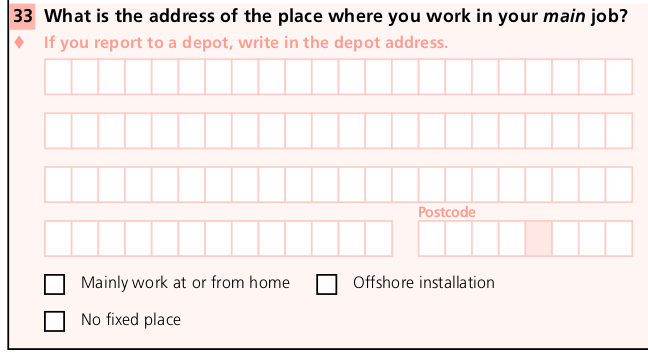
\includegraphics[height=5cm]{q33}
 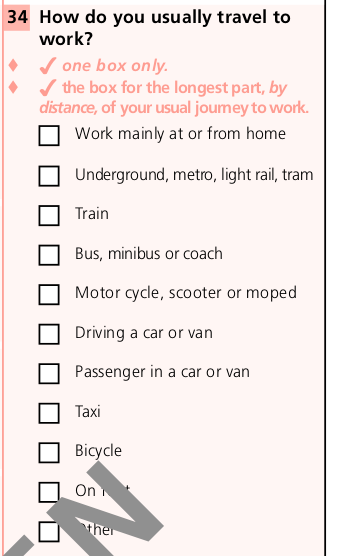
\includegraphics[height=7cm]{q34}
 % cc-trans.png: 1113x529 pixel, 72dpi, 39.26x18.66 cm, bb=0 0 1113 529
 \caption[Questions 33 and 34 of the 2001 UK Census]{Questions 33 and 34 of the
2001 UK Census, which provide information
on mode (left) and distance (right) travelled to work, respectively.}
 \label{fq33}
\end{figure}

These data are available at the individual level through the Sample of
Anonymised Records (SARs) for 1 and 2\% samples of the entire survey.
For the purposes of this study, however, alternative sources of individual
level commuting data were used, to provide additional variables. The main
use of census data, therefore, was as a source of `small area constraints'
(described in \cref{s:defs})
for spatial microsimulation, at various levels of geographic aggregation. 
The main disadvantage of the census
dataset is that it only provides information about a small number of variables
compared with more specific surveys that have lower samples sizes. Only 57
questions were asked in the 2011 Census. By contrast, the number of variables
in the NTS and the USd datasets runs into several hundred.

\subsection{Geographically aggregated data} %Add what's available from 2011!!!
\label{sgeoaggdata}
Census data on commuting is disseminated by Casweb at a range of geographic
scales (\cref{f:scales}) and with a variety of cross-tabulations. Before
forging ahead and describing how the datasets are used, it is worth taking stock
of the scales of geographical aggregation at which they are available.
Consideration of the range
of options at the outset is especially important because research
findings can depend on the size and shapes of geographic zones,
the `areal units' of analysis \citep{Horner2002, Openshaw1983}. Selecting zones
that are too small relative to the study \index{scale} \index{geographic
aggregation}
area can lead to long processing times, messy maps and over-complexity.
Analyses based on overly large zones, on the other hand, can gloss over
spatial variability by presenting space in extensive, homogeneous blocks.
Regardless of the scale of analysis selected, it is important to remember that
\emph{all} analysis based on geographically aggregated data may be susceptible
to the modifiable areal unit problem (MAUP) \citep{Wong2009}.
% {\color{red} (Previous
% paragraph about MAUP deleted --- Robin)}

\begin{figure}
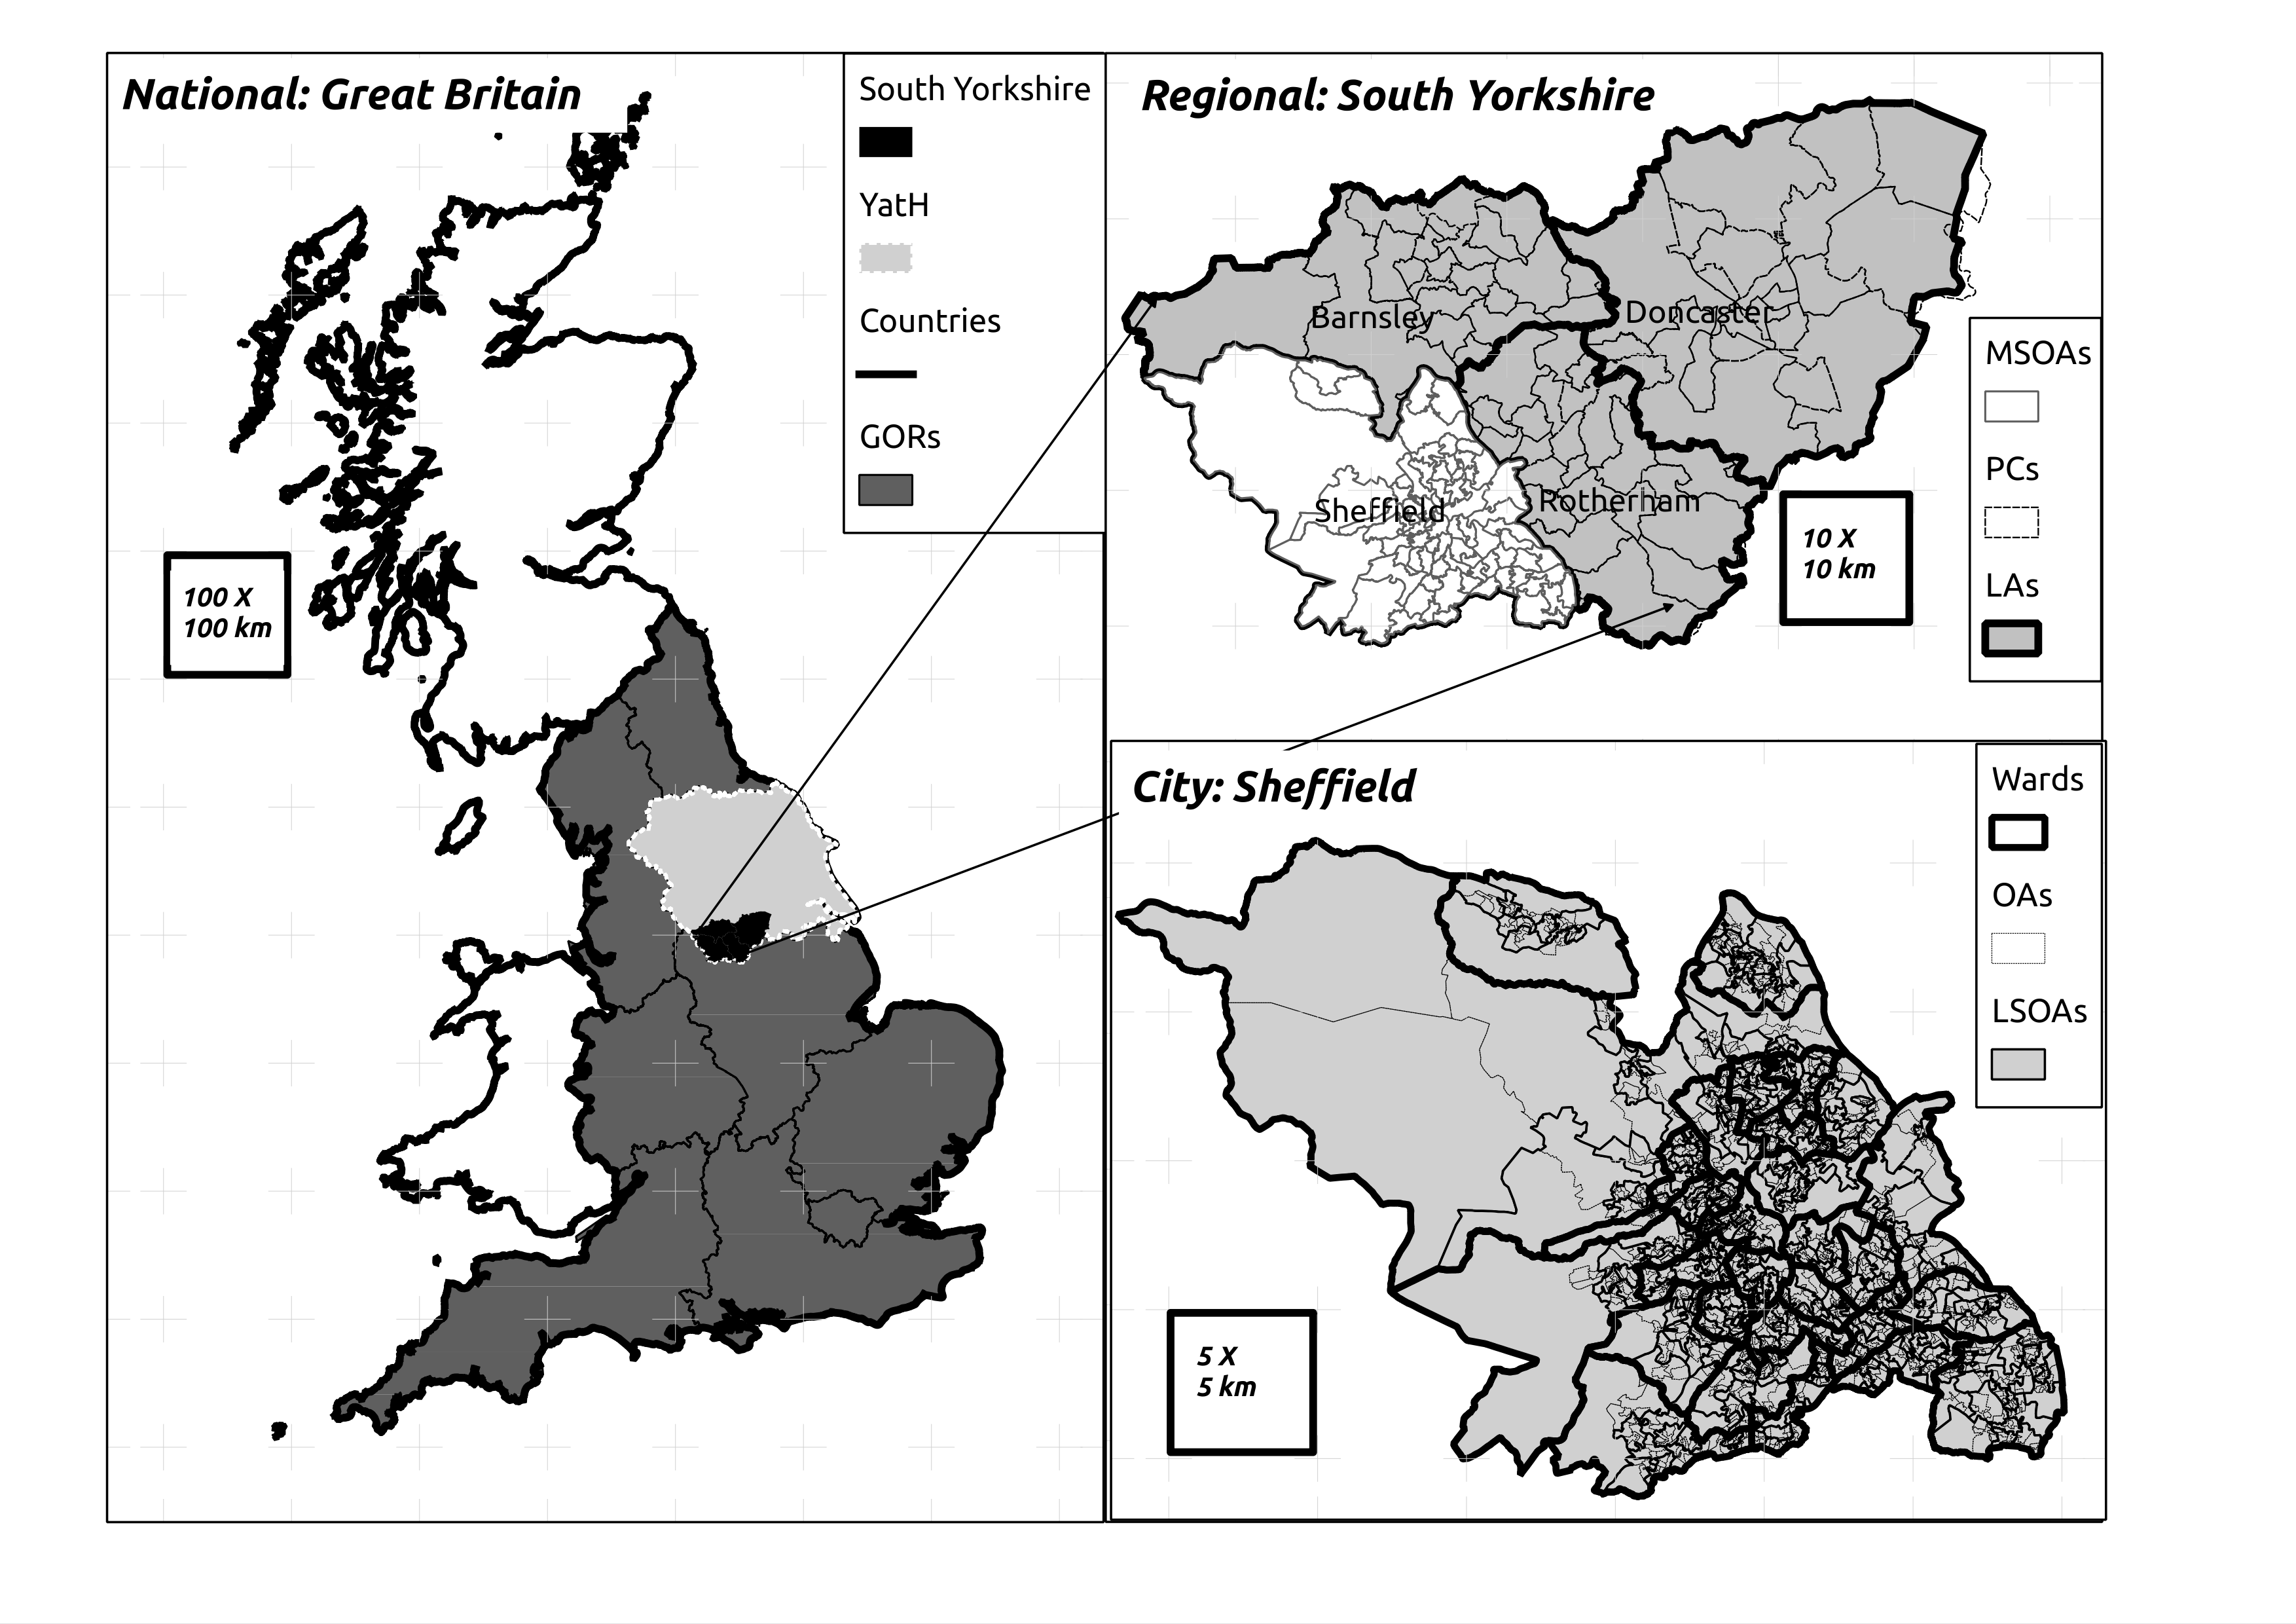
\includegraphics[width=14cm]{scales-map}
\caption[National, regional and city-wide scales of analysis]{National, regional
and city-wide scales of analysis, as illustrated
by a range of administrative boundaries. Yorkshire and the Humber (left),
South Yorkshire (top right) and Sheffield (bottom right)
are the study areas used for this section.}
\label{f:scales}
\end{figure}

% Understanding of the potential impacts of the
% MAUP, and methods for dealing with the problem have improved greatly since the
% 1980s \citep{Sui1999}. However, many studies within
% transport geography continue to follow the tendency of human geographers to
% ``opt for one level of analysis exclusively, without considering the range of
% alternatives'' \citep{Watson1978}. Geographical research on commuting is no
% exception \citep{Horner2002, Li2012}, tending to use only ``a single
% set of analytical [areal] units'' for each case study \citet[p.~40]{Sui1999}.
One of the advantages of spatial microsimulation is that it facilitates
`frame-independent' (scale independent) analysis \citep{Horner2002}. The
results for any particular region --- a table of geo-located individuals equal
in population to the commuting population of the region --- should be roughly
the same in terms of the size of the output file and distributions of
individual level variables, regardless of the scale of analysis. It is
still important to choose an appropriate scale, as lower
geographies will provide more localised information, yet be harder
to analyse and visualise. 
Spatial datasets related to commuting in the UK, and their scales of
dissemination, are outlined
in Table \ref{t:agdata}.\footnote{The administrative acronyms OA, LSOA,
MSOA, and LA refer to Output Areas (which contain $\sim$300 people),
Lower Super Output Areas ($\sim$1600 people), Medium Super Output Ares
($\sim$7000 people) and Local Authorities (more than 100,000 people)
respectively.}

\begin{table}[htbp]
\begin{threeparttable}
\caption[Aggregate data on energy costs of commuting by
scale]{Aggregate data related to the energy costs of transport to
work and the scales at which they are available for South
Yorkshire. The slash symbol (e.g.~in ``Mode/distance'')
represents cross-tabulation. Source: Casweb, unless otherwise stated.}

\begin{tabular}{|l|l|l|l|l|l|}
\hline
Variable & OA & LSOA & MSOA & ST Ward & LA \\ \hline
N. zones in South Yorkshire & \multicolumn{1}{r|}{4278} &
\multicolumn{1}{r|}{845} &
\multicolumn{1}{r|}{173} & \multicolumn{1}{r|}{59} & \multicolumn{1}{r|}{4} \\

Average population & \multicolumn{1}{r|}{296} & \multicolumn{1}{r|}{1450} &
\multicolumn{1}{r|}{7320} & \multicolumn{1}{r|}{21500} &
\multicolumn{1}{r|}{317000} \\
Mode of transport to work & Y\tnote{a} & Y & Y & Y & Y \\
Average distance & N & Y & Y & Y & Y \\
Distance categories & Y\tnote{a} & Y \tnote{c} & Y\tnote{c} & Y & Y \\
Mode/Distance & N & N & N & Y & Y \\
Car access\tnote{b} & Y & Y & Y & Y & Y \\
Domestic energy use\tnote{d} & N & N & Y & N & Y \\
Transport energy use\tnote{d} & N & N & N & N & Y \\
Total energy use\tnote{d} & N & N & N & N & Y \\ \hline
\end{tabular}
\begin{tablenotes}
\begin{footnotesize}
 \item [a] Output area statistics are often unreliable because values less than
3 are randomly allocated the value of 0 or 3. This is problematic for sparsely
populated categories such as those who travel 60 km or more to work.
\item [b] `Car access' refers to the census dataset `cars or vans' which
provides counts for the number of houses with access to no cars, one car etc,
and total number of cars in each area. This is for estimating reliance on
public transport.
\item [c] Data provide by Nomis government data portal, providing various
cross-tabulation options (\url{https://www.nomisweb.co.uk/Default.asp}).
\item [d] Data provided by the Department of Energy and Climate Change (DECC,
from
\url{http://www.decc.gov.uk/en/content/cms/statistics/energy_stats/regional/}).
\end{footnotesize}
\end{tablenotes}
\label{t:agdata}
\end{threeparttable}
\end{table}

As well as being available at different administrative geographies, the datasets
presented in Table \ref{t:agdata} are variable in terms of reliability, their
origin, and times of collection.
Following the `confidentiality principle' of
census data release \citep{Rees2002}, small numbers (3 or below) are allocated
as either 0 or 3 for census data.
This makes cross-tabulated datasets of unusual categories such as `cycles to
work' unreliable at the smallest Output Areas (OA) level.
Census data are the `gold standard' in terms of accuracy
and geographical coverage \citep[p.~4]{Martin2002}.
% : completion rates
% and levels of truth-telling are high for census surveys
% and its completion is a legal obligation for every UK citizen
% .
However, as mentioned earlier, the census lacks details covered by more
specific surveys. Of relevance to energy use, there is no information about the
type of car that car commuters used, or the route distance to work each of
which can have a large impact on overall energy use. The fact that census datasets
are only released every 10 years is a major disadvantage for dynamic analyses
compared with rolling surveys such as the NTS and the USd. It should be noted
that while the data provided by Casweb and Nomis are essentially the same,
% originating from analyses of census data,
the DECC data on energy use was collected in a different way and at a different
time, running from 2005 to 2010, as opposed to 2001.

\emph{Cross-tabulated counts}

Cross-tabulated count data refers to categories which are split up into
subsections. The cross-tabulation mode/distance, for example would contain the
number of car drivers who travel 0-2 km to work, 2-5 km etc.~and the same
sub-categories for every mode of transport. The number of variables (and hence
cells) multiplies with each additional cross-tabulation. To provide another
example, CAS119 (from Nomis) presents mode of travel to work (car, bus etc.) as
cross-tabulated by two other variables --- age and sex.
This provides the potential for more accurate microsimulation (by constraining
by more, cross-tabulated, variables) and a foundation for
validation. Disadvantages of Nomis include the increased likelihood of
empty cells in cross-tabulated data
% % Could mention here that Nomis data is randomised to protect anonymity
% However, priority now is to keep it short and sweet.
and `information overload' for the researcher: it is difficult to analyse and
visualise a 3 way cross-tabulated dataset including more than 100 variables,
such as CAS119, using standard methods of spatial data analysis.

\begin{figure}
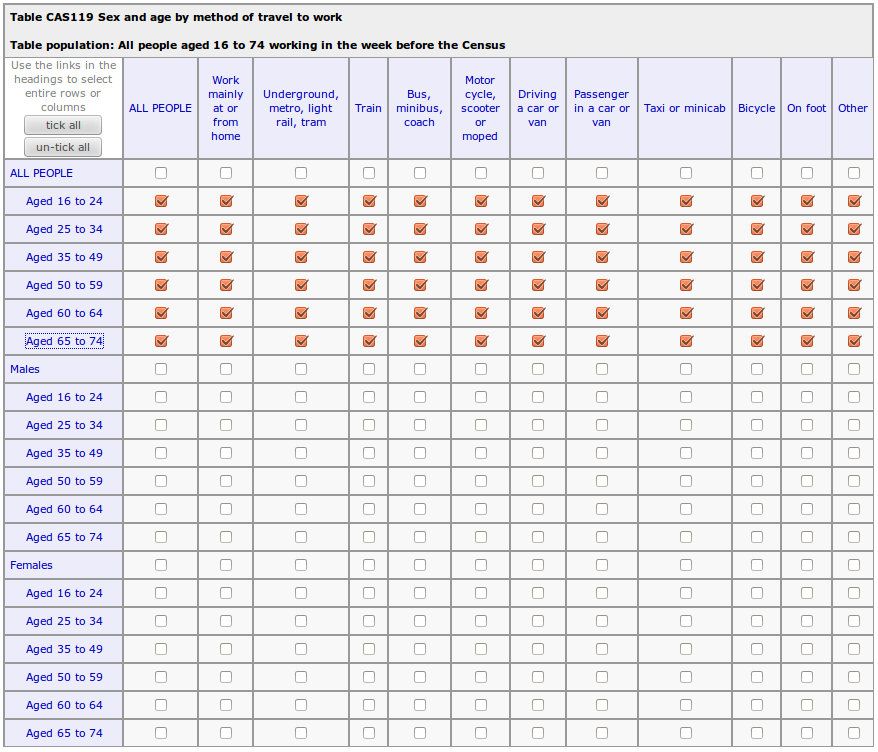
\includegraphics[width=13cm]{cas119}
\caption[Cross-tabulated dataset containing mode/age/sex
variables]{Cross-tabulated dataset containing mode/age/sex variables from Nomis
(dataset CAS119).}
\label{fig:cas119}
\end{figure}
Data size can be a problem: the selected variables presented in
Fig.~\ref{fig:cas119} represent 308,016 cells at the output area for
South Yorkshire\footnote{6 age categories multiplied by 12 mode
categories multiplied by 4,278 output areas.}
and takes up almost a megabyte of
hard-disk space just for Yorkshire and the Humber. All variables, downloaded for
the entirety of England (165,665 OA areas), would take up $\sim$80 Mb of hard
disk space and require a powerful computer for spatial analysis and mapping.
Larger administrative boundaries within a smaller case study area such as South
Yorkshire present no such problems, however, for cross-tabulated data.

Additional cross-tabulated datasets of relevance to commuting are provided by
Nomis and Casweb (the latter via `Census Area Statistics') at each of the
spatial scales presented in Table \ref{t:agdata}, and a few others.\footnote{The
complete set of Geographies at which these data are available via Casweb
is: Country, GOR, 	County, 	Unitary Authority, 	District,
ST Ward, CAS Wards, 	OA.
} A
selection of these cross-tabulated datasets, and an explanation of how they
relate to commuter patterns, is presented below:
\begin{itemize}
 \item  CAS118: Number of employed persons in household/mode/numbers of cars
or vans in household. Useful for investigating rates of intra-household car
sharing, links between car ownership and employment, and household level
microsimulation.
\item CAS120: Sex/age/distance travelled to work. Investigation of the
demographics of people who depend on long-distance commuting.
\item CAS122:	NS-Sec/mode of travel to work. Allows investigation of the
interaction between class and mode of transport to work.
\item CAS121	Sex/distance/mode of travel to work. Which modes are used for
long and short distance trips in each area?
\end{itemize}

\subsection{The Understanding Society dataset} \index{British Household Panel
Survey}  \label{sUSD}
The aggregated census data described above form a solid foundation for analysing
commuting patterns. However, they omit a number of relevant variables
and mask intra-zonal variability.
To perform any kind of microsimulation study, a micro level dataset must
always be found as a starting point: ``Before any attempts can be made at
simulation the first requirement is for a population sample to be obtained
at the micro level'' \citep[p.~147]{Holm1987}. This sample
can be based on a pre-existing
survey data-set, a bespoke survey tailored to the demands of the model, or,
if these options are unavailable, from synthetic populations based on Monte
Carlo sampling techniques. Data on commuting is collected by the government in
surveys, so the first option is used here. 

Table \ref{t:indata} illustrates some important individual level `target
variables' (defined in \cref{s:defs}) that are available through a
single dataset: the
Understanding Society dataset \index{Understanding Society dataset}
(USd).\footnote{Understanding
Society replaces the British Household Panel
Survey (BHPS) as the UK's largest national governmental survey (see
www.understandingsociety.org.uk). The Department for Travel's National Travel
Survey and the Living Costs and Food Survey provide additional options for
individual level variables related to commuting. The USd is the most
comprehensive (with a longitudinal sample size of 50,000), so was the first
option that was used.
}
Many more variables, covering many aspects of life are also available in this
dataset. The most important ones, from the perspective of spatial
microsimulation are the most basic ones: age, sex, socio-economic class, number
of cars in household, hours of work and house tenure. These provide a link to
the aggregated census variables described above via constraint (or `linking')
variables. %%% To be discussed later in the chapter !!! %%%

Crucially for this research, the USd also contains data on travel to work.
In the British Household Panel Survey (BHPS), that preceded the USd, mode of
travel to work and time of travel were the only variables
available, and contained nothing on distance.\footnote{These
variables resulted from the following questions: ``About how much time does it
usually take for you to get to work each
day, door to door?'' and ``And what usually is your main means of travel to
work?''
(\href{
https://www.iser.essex.ac.uk/bhps/documentation/pdf_versions/index.html}{
www.iser.essex.ac.uk/bhps }).
}
% Link to BHPS-in-R.r!!!
However, from 2011 onwards the USd (which replaced the BHPS) contained a
question on distance travelled, resulting in the variable ``workdis''
\citep{ESDS2011}, which is the route distance reported by the respondent, to
the nearest mile. This is the first time distance has been included in any major
British longitudinal survey (Buck, 2011, personal
communication).\footnote{Prof. Nick Buck, director of the UK Longitudinal
Studies Centre, by telephone, 05/10/2011. The National Transport Survey (NTS,
2009) also contains some information on transport to work but is only available
to the public in aggregate forms, and is not comprehensive because it
provides little on non-transport characteristics.
}
However, the
variable has only a 47.2\% completion rate among those who travel to work,
meaning the sample size is reduced from 10,681 to 5,043.
% (See Appendix x on cleaning data, taken from BHPS-in-R.r).
Including the dropping of respondents who do not travel to work (48.0\%), the
cleaning process reduced the sample size of the Understanding Society
dataset by 3/4 from its original value of 22,265 employed people.

\begin{table}[htbp]
\caption[Selected individual level variables related to commuting]{Selected
individual level variables related to commuting,
available from the Understanding Society dataset.}
\begin{tabular}{|p{2.5cm}|p{2.5cm}|p{4cm}|p{4cm}|}
\hline
Attribute & Variable & Measurement & Comment \\ \hline
Type of car & Household variable 146 & Engine size of cars: \hspace{1cm} $< 1.4
,
1.4-1.9 $, or $\ge 2 l$  & Data on additional cars also available \\
\hline
Household income & Household variable 193 & Net household income,
\pounds/month & Equivalised income must be calculated \\ \hline
% Car sharing potential & indresp: envhabit10 & Frequency of car sharing: 5
point
% scale from “always” to “never” & Subjective \\ \hline
Telecommuting potential & Individual level variable 953 & 7 point scale from “no
access”
to “everyday” & Must be linked with type of work \\ \hline
Ease of moving home & Household variable 171 & Number of children (aged 15 or
under) in household   & One indication of how settled household is \\ \hline
\end{tabular}
\label{t:indata}
\end{table}

It should be noted that the USd variables described in Table \ref{t:indata} are
\emph{proxies} of the attributes assigned to them: therefore they should be
interpreted with caution. The propensity of households to move (linked to
commuting via job mobility), for example, does not just depend on the number of
children:\footnote{To
provide another
example, the USd provides three categories of car engine size rather than
describing the exact make and model, a substantial oversimplification from the
perspective of energy use.
}
 it also depends on other factors such as the ownership status of the house,
years left on mortgage, time spent at current location and satisfaction with the
local community \citep{Charlotta2011}. Some of this information is in fact
provided by the USd (in variables `hsownd' and `mglife', at the household level
and `mvyr' and `lkmove' in the individual questionnaire): Table \ref{t:indata}
represents only a snapshot of the available variables. For more detailed
information about personal travel (but less more general data) the
National Travel Survey was analysed.

\subsection{The National Travel Survey} \index{National Travel Survey}
\label{snts}
More detailed information on commuting behaviour is provided by the 2002-2008
National Travel Survey (NTS). This household and individual level survey was
commissioned by the government to better understand transport issues. A
stratified random sample of $\sim$8,000 households each year took place,
resulting in detailed travel diary data for 152,344 (un-weighted) individuals
or $\sim$20,000 in each of the 7 sample years.

The household level dataset is most useful at providing insight into people's
perceptions of their surroundings from a transport perspective. Issues probed
within the 165 variables of the 63,952 row dataset include:
\begin{itemize}
 \item The accessibility of public infrastructure nodes (e.g.~ variable H13,
``Walk time to bus stop'' or H15, ``walk time to railway station'').
\item Quality of the travel network (e.g.~h122: ``Rate the frequency of local
buses'' and  ~h127: ``Rate the provision of local cycle lane/paths [on a 5 point
Likert scale]'').
\item Ownership and availability of vehicles (e.g.~Number of bicycles or
cars/vans (h35a and h55) and h57: ``Household vehicle availability'').
\item Importance of travel in quality of life (e.g.~ variable H148, ``Importance
of public transport in choice of home'').
\item Proximity of essential services:
Journey time to nearest GP, hospital, shopping centre, school, post-office
etc (variables h160 to h168).
\end{itemize}
These variables are not used directly in the spatial microsimulation model
presented here. They could, however, be useful for evaluating the
impact of
environmental factors and household possessions on transport energy use and for
comparing energy use for travel to work with energy use for other types of
transport at the household level. 

At the individual level, the NTS also provides a range of useful
variables, many of which are not available in other surveys. These include basic
social and demographic
details: age, sex, employment status (self employed vs employee), economic
status (full time, part time, unemployed etc.). In addition, via links to the
household level dataset, tenancy, household income (in three bands), social
class (of household representative) and car ownership can also be allocated at
the individual level.
These basic variables are also collected by the Census. This would enable
the NTS to be used as an input micro-dataset for spatial microsimulation models.

The individual level dataset consists of 175 variables which contain more
detailed information about travel habits than any other major British survey.
These interrogate many aspects of individuals' travel experiences, from
expenditure on public transport to driving experience and from frequency of
flights to where they cycle. A selection of the most relevant questions (which
are not directly related to
commuting) are summarised below.
\begin{itemize}
 \item  Variable i182A --- Driving licence (yes, no or provisional): this may
 help separate those who
 do not drive because they \emph{cannot} from those who do not drive out of
choice (although some may choose not to own a driving licence).
 \item I203 --- Access to car (with answers falling into the following 5
categories: company car, main driver, not main driver of household car, car
available but non driver, driver but no car): enables use of car to be linked
to car accessibility.
 \item I283 --- Method of school travel (and many questions about the reasons
for this): enables investigation of the links between mode of travel to work to
be linked with mode of school commute, at different distances.
 \item Frequency of walking and cycling --- would allow researchers to
investigate the link between walking and cycling to work and for other reasons.
If one replaces the other, the energy impact of shift to these modes may be
more positive.
\end{itemize}

As with the household level variables, the main utility of these is adding
subtleties, quantifying uncertainties and demonstrating the complexity of
variables that interact with travel behaviour overall. None of the NTS variables
mentioned so far deal with travel to work directly, however. Commuting data are
provided by variable I180 (``usual means of travel to work'') and I92 (``work
place'', which provides four categories about their work location: a single
location, 2 places (visiting each at least twice per week consecutively),
different places or mostly from home). The main drawback of the NTS dataset
from a commuting perspective is that it does not provide information on the
distance between home and
work directly.\footnote{Data
on trip commuting trip distance is
provided in a separate NTS database entitled `commuting-trips', a small subset
(38 Mb, in .sav format) of the larger (225 Mb) complete `trips' file. Variable
jd provides the most precise data on the responses to this question, to the
nearest tenth of a mile and jdungross provides the rounded average.
Variable j34 provides this data as relatively fine categorical data. 12
variables are provided: ``under 1 mile'', ``1 to under 2 miles'' ... ``200 miles
and over'', with further bin breaks at 3, 5, 10, 20, 15, 25, 35, 50 and 100
miles. This trips provides 44 variables in total on the origin, destination
duration time, distance and (for public transport) costs, with one row allocated
per trip. } %%% More on this pleeease! And add a plot comparing distance dists.
An individual level ``distance to work'' variable can be calculated based on
the
%%% was it??? or no???
trips database, which would enable the NTS dataset to be used as a complete
replacement for the USd dataset in terms of constraint variables.


The main strength of the NTS dataset, that \emph{is} directly related to
commuting and provided directly at the individual level, is its provision of
detail about travel behaviour. Used in addition to the more general USd, it
allows complexities of travel to work to be examined quantitatively.
Quantitative information about travel to work usually oversimplifies of
reality --- person X travels to work by mode of transport Y. Yet in the real
world things are rarely that simple.
% Luke's case study goes here
The NTS
tackles this issue at both individual and trip levels. At the individual level
questions probe the extent to which the same trip to work is a regular event.
Variable I309 provides a binary yes/no answer to the question: ``Possible to
work at home?''. Variable I310 adds subtly to this by providing seven
categorical answers to the question: ``How often work at home?'' ranging from
``3 or more times per week'' to ``less than once a year or never''. The
prevalence of each answer (\cref{ffreq-nts}) becomes useful during attempts to
improve the accuracy of relatively crude energy cost estimates %%% section???
and discussions of the \index{work from home} \index{home working}
reliability of the results. %%%???section
To provide another example, the extent to which mode of travel to work varies
can be explored with the variable i316: ``Journey to work another
way'', which is rated on a 5 level scale from very easy to very difficult.
Subsequent questions ask what the greatest problem with travelling to work by
another mode is (e.g.~cost of public transport) and main reason for using/not
using the car for the daily commute. Each of these questions helps to
understand the likelihood of modal shift away from the car and the factors
impeding this shift in scenarios of the future.
\begin{figure}
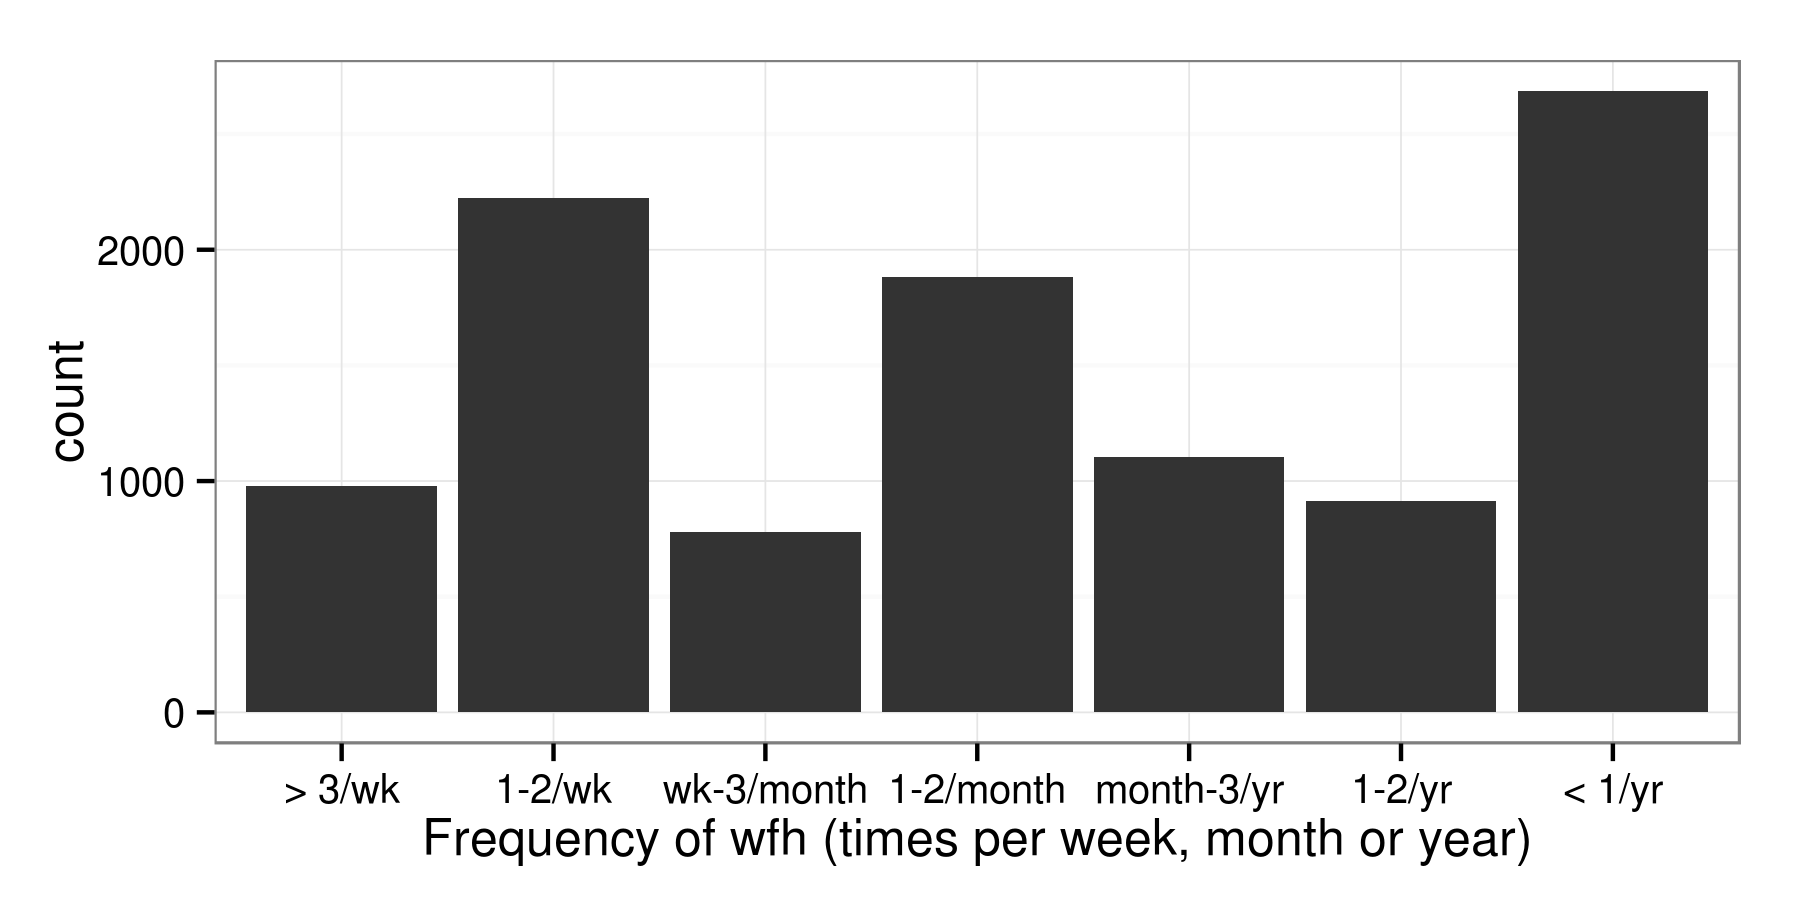
\includegraphics[width=14cm]{freq-nts}
\caption[Bar-plot of frequency of working from home]{Bar-plot of frequency of
working from home (wfh) in the NTS, 2002-2008. Note: only 7\% of the
individual level sample answered this question; around half of the
non-respondents do not work.}
\label{ffreq-nts}
\end{figure}

At the trip level, the NTS contains the following data that can add subtlety
and complexity to our understandings of travel to work. A selection of the
variables that do this are:
\begin{itemize}
 \item D1, J31 and J31A: Journey day and time. This can provide information
about likely level of congestion of work trips on average, and compared with
other trips.
 \item J23: Number of stages. This data mitigates against the simplistic idea,
reinforced by many questionnaires, that all trips consist of only one stage and
one form of transport. The prevalence of multi-stage trips can be investigated
using this variable and, in even finer detail, using the `stages' dataset which
breaks every trip up into its constituent stages.	
 \item JTOTCOST: Total cost of public transport trips. This variable provides
an insight into the costs of public transport and, if the costs of alternative
modes are estimated, the changes that would make more efficient modes more
efficient than driving financially. 
\end{itemize}

`Zooming in' in even further, data on the individual stages taken and vehicles
used for each trip is provided by the NTS in separate files, linked by multiple
(e.g.~household, individual) IDs. The `stages' file 
provides 2.2 million rows of data (only 5\% more than the trips dataset, as
96.7\% of trips taken consist of just a single stage) on occupancy, parking and
even the cost of parking. Clearly, this dataset is invaluable for identifying
the types of multi-stage trip in travel to work, and how these impact on the
energy cost estimates calculated via the assumption that all trips to or from
work consist of just one stage. The `vehicles' dataset contains only 5 types of 
motorised vehicle, including cars, motorcycles/scooter/moped,
``landrover/jeep'', ``light van'' or other. The type of bicycle used to travel
to work is not included, making it impossible to accurately estimate the
embodied energy costs of cycling to work based on the NTS dataset.
Surprisingly, details on the engine size is not provided, although this is not
an issue from an energy use perspective as the CO$_{2}$ band of the vehicle
(which can be converted into energy efficiency estimates) %%%??? Where
is included (in variable V164b). Other relevant variables from the vehicle
dataset include annual mileage (V46), annual commuting mileage (V140) --- these
could be used to determine the extent to which people are dependent on their
cars for commuting, compared with other reasons for trips --- and age of car
(V91a).

The final feature of the NTS dataset to consider is its geographic coverage. It
is a stratified sample within Great Britain. It does contain some geographic
information at the household level, about the type of area in which the
household is based (variable h154a).\footnote{The following 6 categories are
provided:
 Met built-up areas,
 Other urban over 250K,
 Urban over 25K to 250K,
 Urban over 10K to 25K,
 Urban over 3K to 10K,
 Rural.}
Also, the region of each respondent can be inferred by linking individual and
household ids to variable J57G (GOR of trip origin) of the trips dataset.
The NTS dataset has an impressive response rate to key question which tend to
have a lot of NA values, and are very patchy. This would allow an
additional constraint variable to be used for individual level NTS data as an
input into a spatial microsimulation model.

\subsection{Other commuting datasets}
Internationally, the availability of commuting data varies greatly.
This is important, because it can frustrate attempts to compare commuting
patterns across nations. However, if the methods
are to make a major contribution, it should be possible to implement them
worldwide. This depends on access to appropriate data.
Using the aforementioned UK data as a benchmark, Dutch and Colombian datasets
will be evaluated in terms of their suitability for the spatial microsimulation
methods set out below. These datasets were selected because they represent
very different levels of detail, aggregation and availability.

The Dutch data (shown in \cref{sdutchdata}) is provided to the
public\footnote{See {\color{blue}\href{http://statline.cbs.nl/StatWeb/publication/?DM=SLNL&PA=81129ned&D1=0-1,3&D2=0&D3=a&D4=1&D5=0-12&D6=a&HDR=T&STB=G1,G2,G3,G4,G5&VW=T}{http://statline.cbs.nl}},
(full link embedded in the pdf version of this thesis.)} at a
very high level of aggregation. The following attributes are provided for
each mode of transport for each area to two decimal places:
\begin{itemize}
 \item the proportion of all commuters travelling by each mode
 \item average distance of trip
 \item average time per trip
\end{itemize}
The Netherlands data publication policy can be characterised as providing
a very high level of accessibility, but for quite low quality data: it would
not be possible to use this dataset as the basis of a spatial microsimulation
model because, even if socio-demographic constraints were obtained, the
information is provided as averages, telling us nothing about the distribution
of trip distances in each area.
For more detailed geographically aggregated, one would have to
manually aggregate the Dutch equivalent of the National Travel
Survey.\footnote{Piet Rietveld, personal communication.
In fact, there is a plan to do precisely this to provide data to help
explain the differences between English and Dutch energy use, described in
\cref{sinternational}.}
However, the Dutch data does allow for calculation of energy costs, as both
mode, distances and proportions are available (\cref{sinternational}).

On the other extreme, many geo-referenced micro level datasets on
commuting behaviour have been collected. These are generally small in geographical
coverage (at
least relative to the nationwide aggregate level commuting datasets
collected through national censuses) and sometimes in scope also (for example,
it is very common for large organisations to conduct travel surveys of their
staffs' travel patterns). In many cases, a precise geo-reference is allocated
to each individual participating in the survey, although this dataset is generally
not released due to its
sensitivity.\footnote{A
potential case study for this thesis was to take data from the Ordnance Survey's
travel survey as the basis for assessing the energy impacts of organisation level
change. This did not materialise in part due to time constraints and in part
due to concern over access to the geo-referenced individual level data.
}
A very large and detailed example of a geo-referenced individual level dataset
is the \emph{Encuesta de Movilidad de Bogota 2011} \citep{bogota2012}, in which 16,157 `valid'
questionnaires were collected. In addition to questions about travel
(mode, distance and frequency of travel to work and other places), a
range of socio-economic details were collected, including type of housing,
social class, income, `motorisation' (access to cars, motorbikes and bicycles)
and level of education. Unsurprisingly this dataset is not available publicly,
but is available to Colombian researchers with international collaborators
(Ana Moreno Monroy, personal communication). To some extent such a rich dataset
would render the process of generating spatial microdata unnecessary
(although such datasets could be very useful for validation and testing of
these methods). However, the methods of analysis used to interpret the
datasets presented in the latter sections of this chapter and in \cref{s:workdes}
could well be applicable to these valuable micro level datasets.

\section{Geographical data: infrastructure and environment} \label{sadditional}
The datasets presented so far, on energy use of personal travel and commuting
behaviour, are sufficient to calculate the energy costs of commuting at
individual and aggregate levels. The scope of this work extends beyond mere
description, however. Additional input information is required to explain \emph{why}
commuting costs are as they are and to determine the factors likely to
influence the energy costs of commuting beyond those considered so far. These
additional data are classified into infrastructure and topography,
%  geographically inferred data about accessibility
and
remoteness.
%%% May want to say something about additional individual level vars too.

% \subsection{Socio-economic variables} % Add this later
\subsection{Infrastructure}
As discussed further in \cref{scircuity}, the Euclidean distances reported in
the census constraint variable categories (0 - 2 km; 2 - 5 km etc.) are often
not the same as the actual distance travelled to work. This is due to many
reasons, many of them behavioural.
Trip chaining (e.g.~taking a detour on the return journey from
work to do the shopping or on the way there to `drop off the kids'), habitual
use of a certain non-optimum route to work or even preference for
certain parking spaces can all affect circuity. However, infrastructure also
has a large, probably dominant, role to play in determining
how far people \emph{actually} travel to
work relative to the linear distance between home and work. In most cases it is
physically
impossible to travel from A to B in a straight line across an urban area due to
various impassible objects that lie in the way, such as building, fences and
rivers (for all modes of transport) and one-way streets, pedestrianised zones,
prohibitive congestion charges and bollards (for cars). Public transport is the
most constrained geographically, as buses and railed vehicles can only follow
pre-defined paths. Thus, although trains (and to a limited extent buses, when
dedicated bus lanes are present) tend to take more direct routes into the
centre of cities, this does not guarantee that trips by these modes will be
less circuitous than car travel.

Theoretically, the infrastructure on which every mode of transport can usefully
be thought of as a set of points and one-dimensional lines that overlay the
2D geographical surface. %%% Add figure here. And systems of infrastructure
This is reflected in available data on transport
networks: they are
a complex interacting masses of lines (representing the guideways) and points
(intersections between these lines, places to enter the network such as
train and bus stations and motorway link roads). In order to differentiate
between the different transport systems, they can be represented as
completely separate (implicitly non-interacting) layers
(\cref{fnetworks-schematic}). Alternatively,
attributes can be assigned to each
line and point on the entire transport network that includes all nodes and
lines from all networks. These attributes (when present) can be used to
determine the modes that
are able to travel on each, the size of the pathway, information about speed
of travel and, in some cases, direction of travel and other qualities.
With the growth of internet-connected monitoring systems, %% ref
`live' attributes are increasingly feasible (although not yet available in any
dataset the author knows of), such as frequency and destination of departures
and congestion.

\begin{figure}[h]
 \begin{center}
 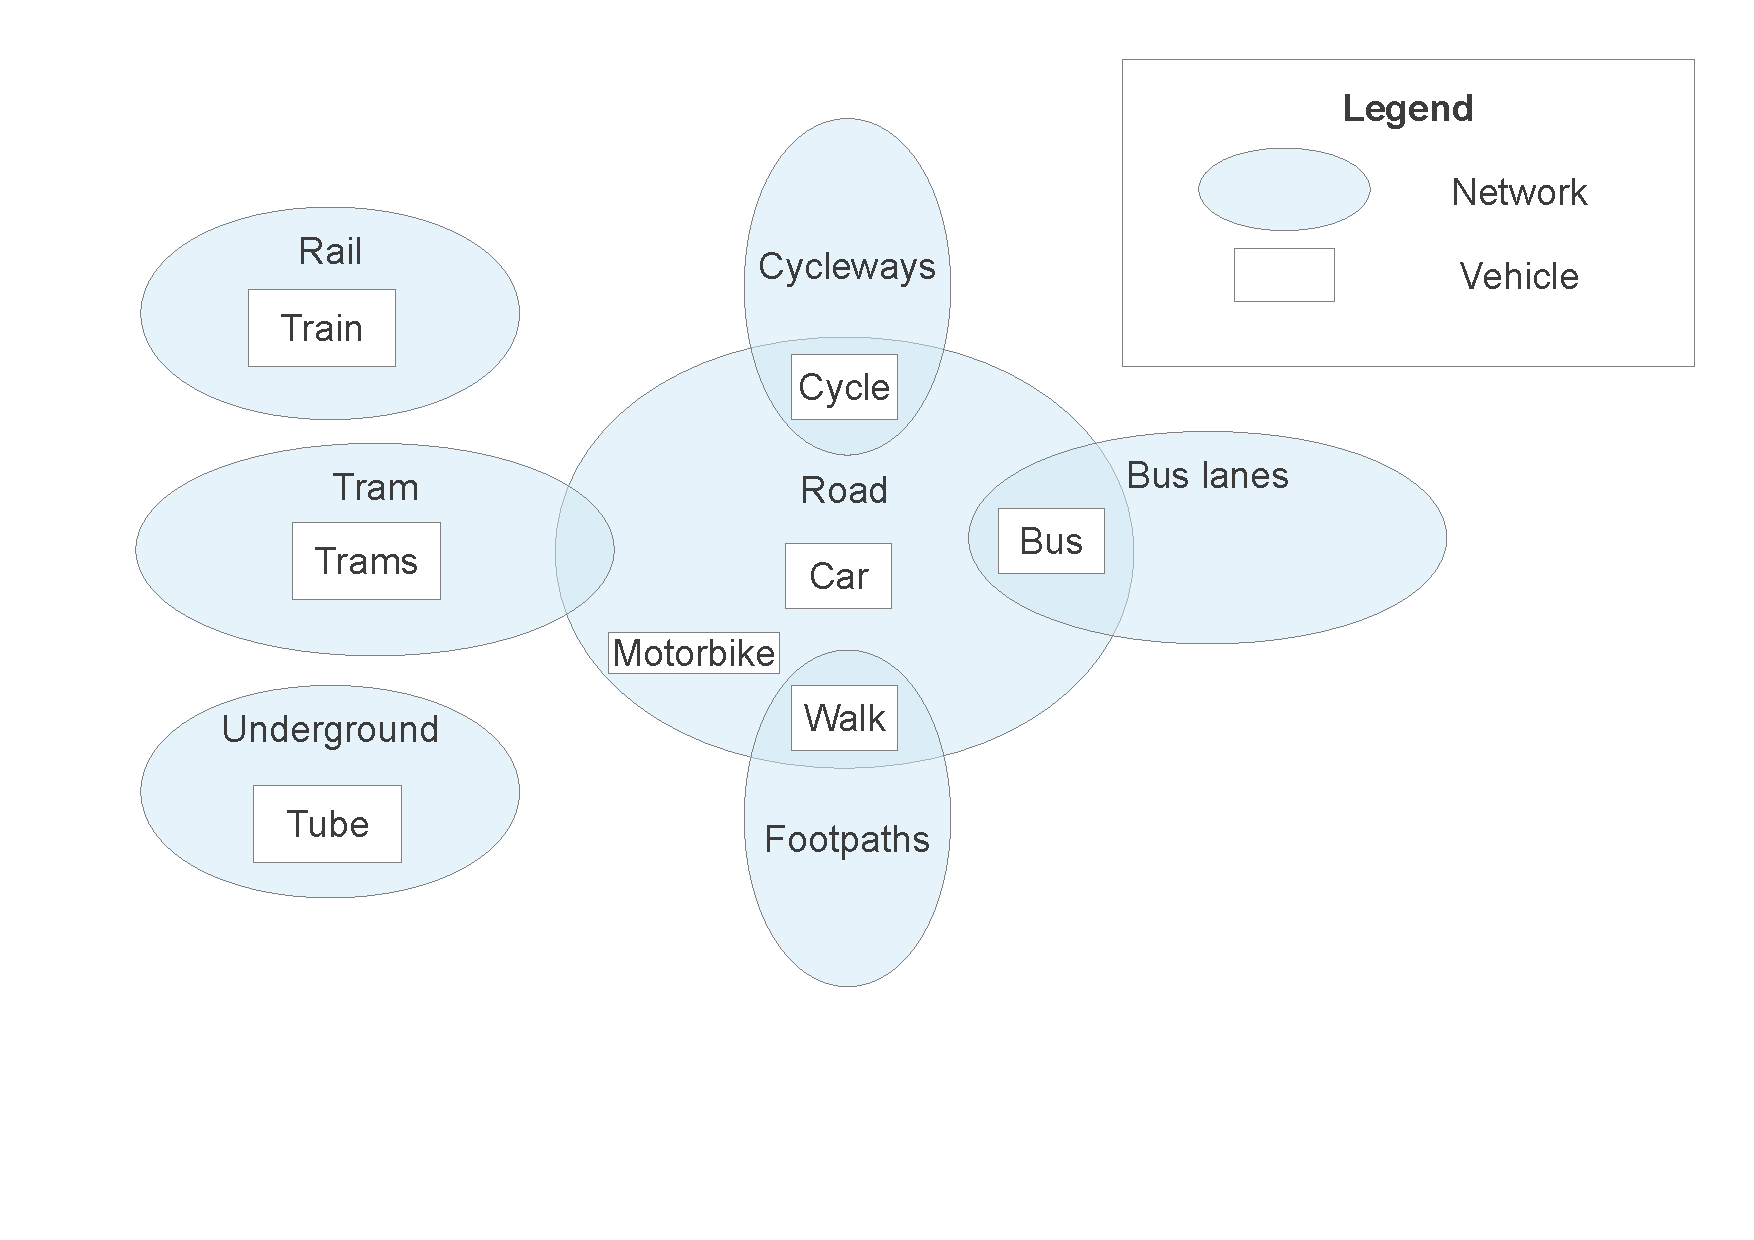
\includegraphics[width=15 cm]{networks-schematic}\end{center}
 % cc-trans.png: 1113x529 pixel, 72dpi, 39.26x18.66 cm, bb=0 0 1113 529
 \caption[Schematic of transport networks and vehicles]{Schematic of main
transport networks used for personal travel and the vehicles that can use them.
Diagram based on \citet{Bolbol2013}.}
 \label{fnetworks-schematic}
\end{figure}


Clearly, this is a complex body of information, and different datasets deal
with it differently (\cref{tnets}). %%% Table on datasets of transport inf.
Only the top three data sources in \cref{tnets} are available free for academic
purposes; these are illustrated in \cref{fosm-trans} to \cref{fitn-master}.
Each of these data sources has its advantages and disadvantages, the most
relevant of which (for the purposes of analysing energy use in personal travel)
will be briefly discussed.



\begin{table}[htbp]
\caption{Comparison of data sources for travel networks}
\begin{tabular}{lp{2cm}p{6 cm}l}
\toprule
Network data source & Networks covered & Key attributes & Availability \\
\midrule
Open Street Map & All & Frequent updated, routing-compatible, official and
unofficial & Free \\
Meridian 2 & Road, rail & Lightweight ($<$ 1 Gb for all UK), national coverage &
Via Edina \\
Mastermap ITN & Road, pedestrian & Large ($\sim$100 Gb for all UK), detailed
with routing & Via Edina \\
ITN Urban Paths & Pedestrian, cycle & Large, detailed map of UK's urban paths
and cycleways & Priced \\ \bottomrule
\end{tabular}
\label{tnets}
\end{table}

\begin{figure}[h]
 \begin{center}
 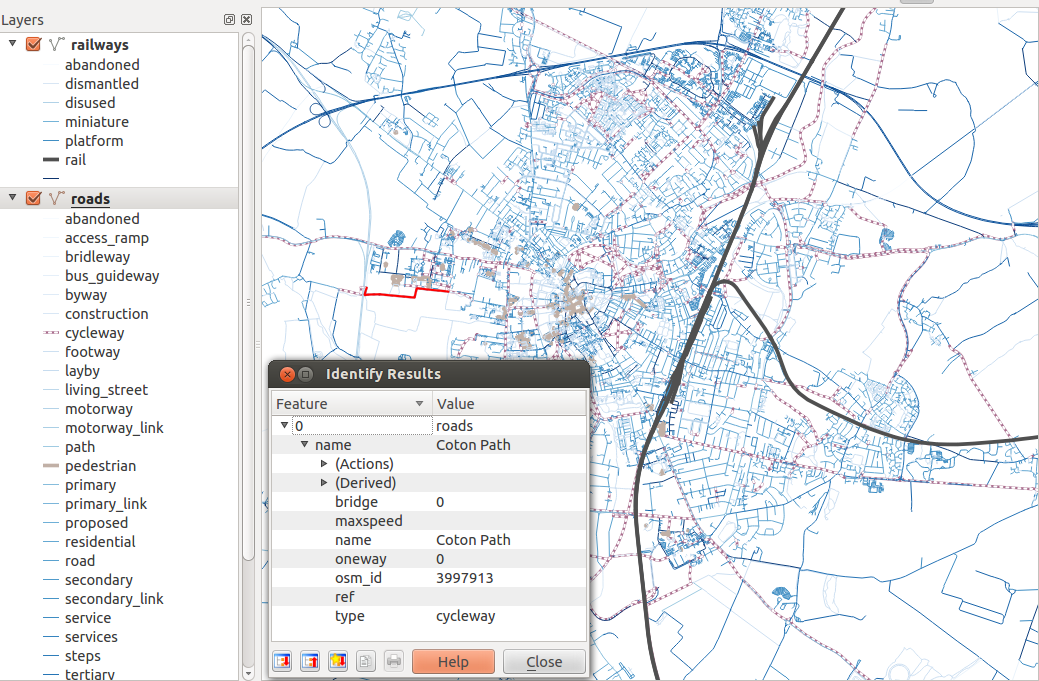
\includegraphics[width=15 cm]{osm-trans}\end{center}
 % cc-trans.png: 1113x529 pixel, 72dpi, 39.26x18.66 cm, bb=0 0 1113 529
 \caption{Visualisation of the OSM data source of the transport network.}
 \label{fosm-trans}
\end{figure}

\begin{figure}[h]
 \begin{center}
 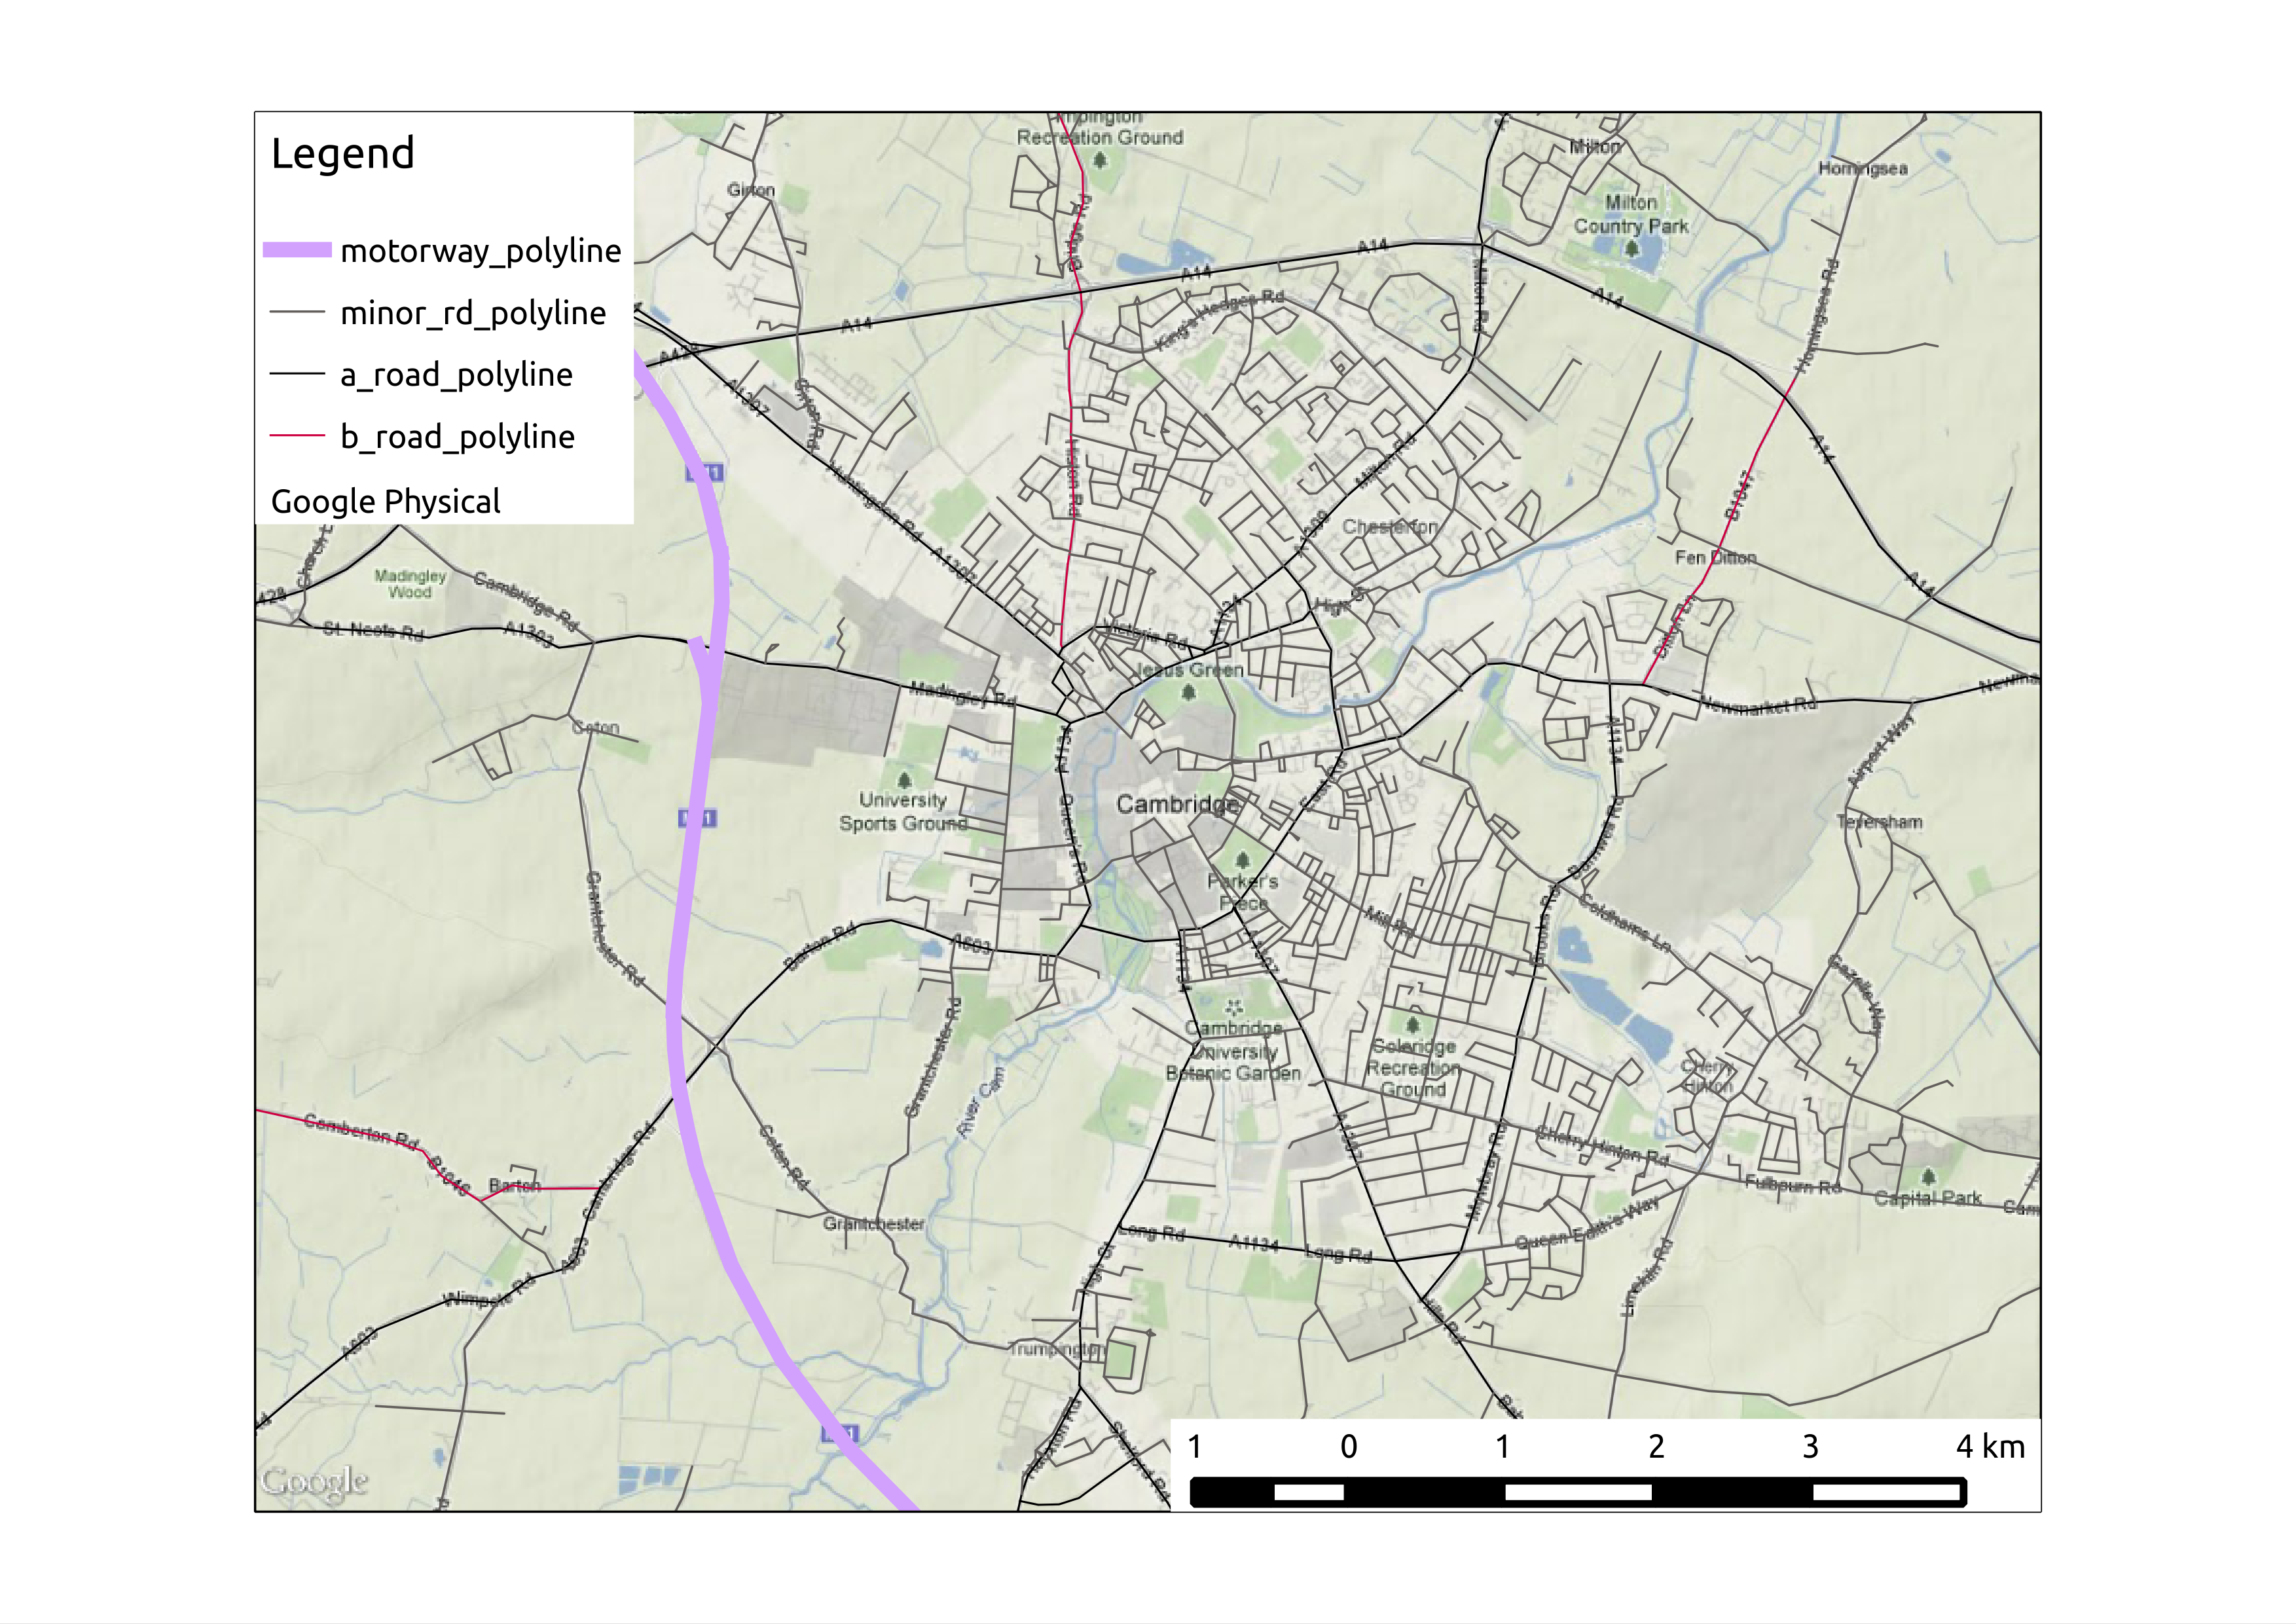
\includegraphics[width=15 cm]{cam-merid2}\end{center}
 % cc-trans.png: 1113x529 pixel, 72dpi, 39.26x18.66 cm, bb=0 0 1113 529
 \caption{The Meridian 2 transport network dataset.}
 \label{fcam-merid2}
\end{figure}

\begin{figure}[h]
 \begin{center}
 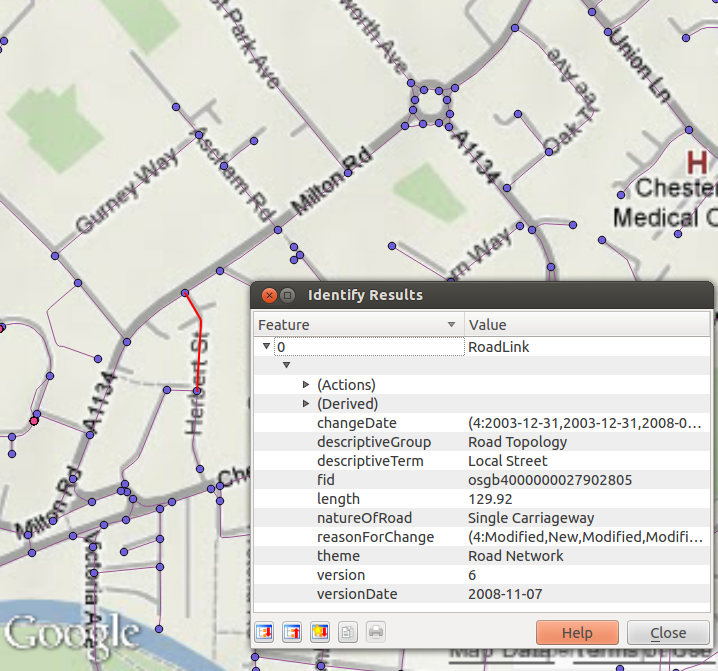
\includegraphics[width=15 cm]{itn-master}\end{center}
 % cc-trans.png: 1113x529 pixel, 72dpi, 39.26x18.66 cm, bb=0 0 1113 529
 \caption{The Ordnance Survey's Integrated Travel Network dataset.}
 \label{fitn-master}
\end{figure}

The Open Street Map dataset is the most suitable `on paper' due to its coverage
of all transport systems in a single file, its level of detail (between the two
free Ordnance Survey offerings: not so large as to make it unwieldy; not too
small to lack detail) and frequent rate of update. Another major advantage of
the OSM dataset is its global coverage: this means that analyses conducted on
it for one country can easily be replicated anywhere in the world. This is not
the case with the Ordnance Survey datasets, as they are proprietary (not
available to non-academic or foreign users) and unique to the UK.

The Ordnance Survey datasets do offer some advantages, however. These can be
summarised as reliability, stability and links to policy makers. All data
entries into the Ordnance Survey system are conducted by professionals who have
been formally trained, and operate to carefully defined standards. OSM data, by
contrast, can be added by anyone with an internet connection. This
`democratisation' of data offers various auxiliary benefits to its participants
\citep{Foresman2008} but also raises issues of data quality. How can one trust
the location and attributes of pathways on a map if they were entered by
amateurs? This is not a question that will be tackled here, but the interested
reader is directed towards the University of Nottingam's OSM-GB (Open Street
Map Great Britain) project\footnote{This project combines OSM data with
information from official sources aims to measure and improve the
quality of the OSM database. See http://www.osmgb.org.uk/ for more detail and
to see their map.} and an academic paper on the subject \citep{Haklay2010}.
\citet{Haklay2010} notes the lack of systematic studies comparing the quality
of traditional and open source (referred to as `volunteered geographic
information') approaches to maps, and sets-out to fill the research gap. It
was found that datasets derived from OSM are generally accurate, especially for large
infrastructures such as motorways, which had an 80\% overlap with the Ordnance
Survey data for 2008 data. However, inconsistencies in the quality of OSM data
were also noted, with rural and deprived areas tending to be more poorly represented in
terms of the existence of objects and the accuracy of their attributes.
Quality of digitisation ranged from ``fairly sloppy in the area of Highgate''
to ``consistent and careful in South Norwood'' \citep[p.~699]{Haklay2010}.
Large errors were far rarer than small ones and overall the OSM
dataset was evaluated as being of `very good' quality.

The second major concern is stability: because the OSM dataset is
continually being updated, it is in constant flux. While most of these changes
are small, and unlikely to alter the results of a particular routing operation,
larger changes do sometimes occur. This is because every aspect of OSM is open
to debate and change. There are, for example, around 5,000 object categories and
growing for OSM objects and users are continuously adding new ones and debating
the structure of the database.\footnote{See
\href{http://wiki.openstreetmap.org/wiki/Map_Features}{
http://wiki.openstreetmap.org/}.} The same issue also applies to the
centralised Ordnance Survey datasets, although these update in a more
systematic manner.

The final point to consider is usability. While OSM datasets are available
worldwide, it is not the standard dataset in use by local planning departments,
which generally have institutional access to Ordnance Survey data. The 
OSM data source is generally also more difficult for non-expert users to find and
download.\footnote{The
OSM transport dataset presented in \cref{fosm-trans}, for example, was not
accessed directly as the .osm file in which the dataset is typically
stored due to problems with downloading, extracting and loading the files in
QGIS. Instead, pre-processed shapefiles, derived from the original OSM data
were downloaded from
{download.bbbike.org}{
http://download.bbbike.org/osm/bbbike/Cambridge/}. Geofabrik.de, and cloudmade
also offer OSM data in forms that are more user friendly for desktop GIS users.
(OSM is well suited to use in geo-databases such as PostGIS.)} Therefore,
one could argue, analyses conducted using the official datasets will be more
likely to be used officially. Of course, this point will vary from organisation
to organisation and methods applicable to one network dataset are generally
applicable to others. In OSM's favour, public administrations in the UK have
recently been recommended to use open source alternatives wherever possible, so
the perception that only official sources are valid may
fade.\footnote{These
recommendations were published in the Government Service Design Manual, as
reported in the story ``New UK government manual for public administrations
promotes open source'' by \href{https://joinup.ec.europa.eu/}{
https://joinup.ec.europa.eu/news/new-uk-government-manual-public-administrations
-promotes-open-source}.}

Consideration of these points led OSM to be the favoured source for most
applications due to its comprehensive coverage of transport networks in a
single file and wide range of attributes for every transport path and node. The
Meridian 2 dataset seems to be best suited for road coverage over large areas
and is ideal for investigating road accessibility of different locations and
network distances by car, as it is available in a handful of polygons for the
entire country. Finally, Ordnance Survey's ITN and Urban Paths layers should be
useful for low level analysis of likely routes of non-motorised modes. However, the
former was found to be difficult to use
% \footnote{97 tiles were downloaded
% for the wider Cambridge area to investigate this dataset. Loading the .gml file
% in QGIS took over a minute and eventually crashed the computer.}
and the latter appears to be unavailable under an academic licence.

\subsection{Topographic data}
Topography is potentially useful both as an explanatory variable of
non-motorised travel and an input into calculations of energy use, due the
addition energy use of driving
uphill compared with driving on the flat.\footnote{This
energy could theoretically
be regained via regenerative breaking. This technology is currently available
in  only a handful of models, and their ``charge/discharge capabilities are
limited'' \citep{Clarke2010}. Due to the added cost and complexity of
regenerative braking systems, their commercialisation for cars and other
vehicles is deemed to be long-way off (if it ever takes off).
}
The extra mechanical energy use of vertical displacement is the same as the
potential energy (PE, measured in Joules) gained by climbing:
\begin{equation}
 PE = mgh
\end{equation}
which is determined by the mass of the vehicle ($m$, in kg), the gravitational
constant ($g$ --- $\sim$10 m/s$^2$ on Earth) and height gained ($h$, in meters).

Topographic datasets for the UK are available from the following sources,
ranging from the coarsest to the finest:
\begin{itemize}
\item The Advanced Spaceborne Thermal Emission and Reflection Radiometer
(ASTER) sensor mounted on the Space Shuttle has produced a dataset that has been
analysed by the Japanese and US space agencies. This has resulted in the Global
Digital Elevation Model Version 2 (GDEM V2). The GDEM has global coverage, a 30
meter resolution, and is free to download from a handful of 
websites, providing a user account and reason for download are
provided.\footnote{See the
following hyperlinks: \href{http://gdex.cr.usgs.gov/gdex/}{cdex.cr.usgs.gov},
\href{http://reverb.echo.nasa.gov/reverb/}{http://reverb.echo.nasa.gov} and
\href{http://www.jspacesystems.or.jp/ersdac/GDEM/E/index.html}
{http://www.jspacesystems.or.jp}. A digital elevation dataset was successfully
downloaded from the first site.} The dataset forms the basis of digital
elevation model used by Google Earth and other Google products.
\item The Ordnance Survey provides height data, either as contour lines or as
interpolated points, for the entirety of the UK and Ireland. The former has a 5
m vertical resolution with an error margin of 2.5 m; the latter has a spatial
resolution of 10 m and an accuracy that depends on the complexity of the
terrain from with points are interpolated.
 \item To improve its flood analysis capabilities, the Environment Agency paid
for a private company to produce high quality LIDAR (light detection and
ranging) data for the majority of the island of Great Britain. The data can be
ordered from the Geomatics website at 25 cm, 50 cm, 1 m, and 2 m resolution, as
either a digital terrain model (DTM, with buildings and vegetation included) or
as a surface model (DSM, representing the `bare' surface). The coverage
increases from less than 1\% for the 25 cm data (for areas most at risk from
flooding) to around 95\% for the 2 m data. The data can be downloaded
commercially for \pounds100 per square kilometre, or free for non-commercial purposes.
\end{itemize}
These datasets were not used directly in the thesis.
Their inclusion could, however, provide background and interesting avenues
for further research for example as a predictor of
the rate of cycling and walking or as a local modifier of energy economy estimates.
% !!! Change this is you use topo data !!!

% \subsection{Estimating accessibility} \label{sgeoinf}
% Some individual level data can be inferred  based on aggregate level data.
% The number of people who commute in the same direction, for example, can be
% derived from commuting flow data provided by Nomis.
% %\footnote{Where to find this
% %data... }
% % by allocating workplace basec on this information.
% This additional level of detail, about \emph{where} people travel to and from
% may well be relevant for decision makers. Simulation of the potential for
% trip sharing or for the increased uptake of non-motorised modes along
% frequently used home-work corridors, for example, could harness this data. The
% `where' question also has strong practical applications, as new infrastructure
% projects such as new bicycle paths rely on data on where people travel from and
% to. The inclusion of direction of commute, via flow data, is tackled in
% \cref{sflow}. This is the type of geographical inference discussed in this
% section, but applied to variables other than those covered by flow--data and
% spatial microsimulation.
% 
% Many variables related to the energy costs of commuting are not
% provided `off the shelf' in official data such as census aggregates. Many of
% these variables (e.g.~average distance to bus stops) have a spatial element, and
% can therefore be inferred from geographic data using computerised calculation.
% Spatial microsimulation performs such inference for individual level variables
% % (hence its alternative name: small area \emph{estimation})
% by combining geographical data, such as that presented in table
% \ref{t:agdata}, with non-geographical microdata (e.g.~see Table \ref{t:indata}).
% This is a central method of the PhD, and is
% described in detail in \cref{setsim}.
% The methods of geographic inference described in this section are simpler. To
% take one example, let us consider the example of proximity to bus stops. As
% mentioned, this is a variable provided at the national level by the NTS, but
% lacks any geographic coverage. Taking an arbitrary Local Authority (data and
% analysis at the national scale would be unwieldy) the input data is available
% from two sources. Open Street Map (OSM) data provides a dynamic yet not
% comprehensive list of bus stops over any area on Earth (Table x). The official
% dataset is more reliable (Table x, Fig. x).
% %%%!!! Priority level: not high. Really good test of speed and skill as qgeo!
% 
% % Other examples: accessibility rank of cycle schemes; public transport
% % Also, 'remoteness' etc sure fit into this section.
% !!! \emph{Here the intention is to highlight explanatory variables and
% quantitative methods} !!!

\subsection{Remoteness} \index{remoteness} \label{sremotness}
% Or area classifications and remoteness or geographically inferred ...
In addition to the transport infrastructure of each area, remoteness was
expected to influence
commuter energy use, primarily via distance travelled and car dependence.
% As outlined in \cref{chapter2}, past literature also supports this hypothesis
% \citep{x,yz}.
%%%! REALLY??? add in cross-ref here.
Intuitively, remote areas are likely to have high energy costs simply by virtue
of the average distance to jobs. Distance to nearest urban centre is a
potentially useful proxy to measure this type of remoteness. This, and
related classification of areas, form the basis of this section.  
The example described applies to medium super output areas (MSOAs) in Yorkshire
and the Humber; the same method could just as easily be applied other
geographies or regions.

The starting point for this is analysis to consider the opposite of remoteness:
living within a city centre. City inhabitants are clearly not isolated in terms
of amenities and social connection, but living in a city does not
actually guarantee proximity to good jobs.\footnote{A good
example of this is Hull, which has the highest unemployment rate of any UK city:
8.7\% ofthe adult population was receiving unemployment benefit as of March 2013
\citep{SimonRog}.
}
To tackle this issue the concept of `employment centre', meaning an area 
with a high concentration of jobs,  was used
against which to measure remoteness. In order to calculate the remoteness of
each MSOA area from employment centres,
it was first necessary to define what constitutes an employment centre and what
does not. Of course, the availability of jobs is not determined by the
Euclidean distance to one dimensional points on the map: employment density
varies continuously over space depending on the location of businesses, schools
and other major employers (\cref{flows2bigemps}). However, employment centres
can provide a neat simplification of reality, a model to simplify and help
understand the complexity of the labour-market commuting interaction.

\begin{figure}[h]
 \begin{center}
 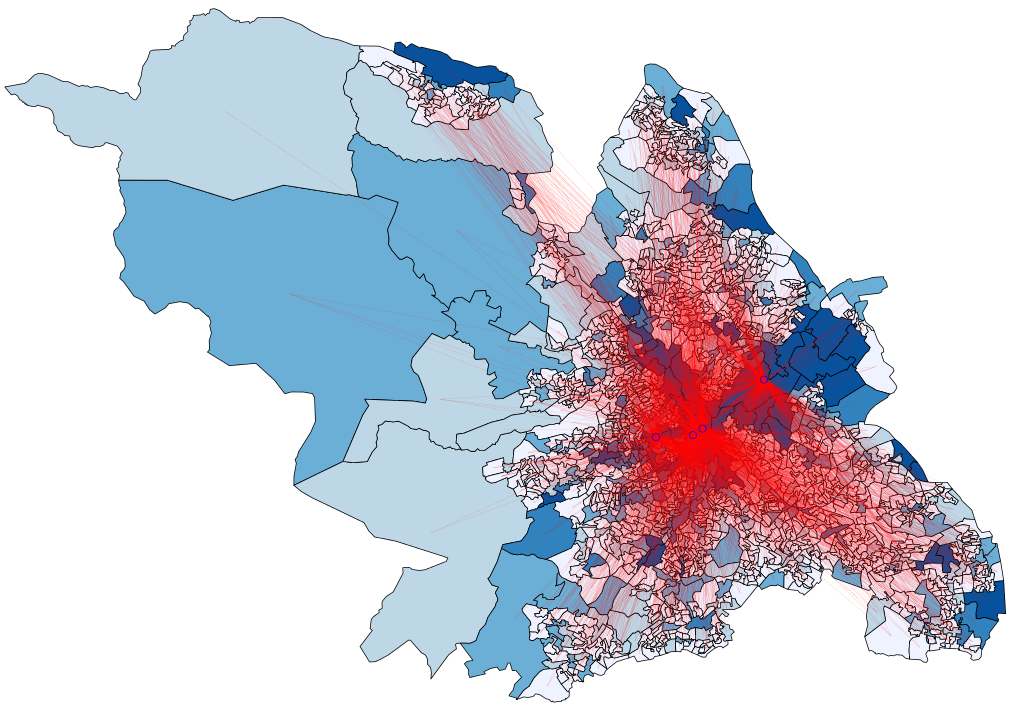
\includegraphics[width=16 cm]{flows2bigemps}\end{center}
 % cc-trans.png: 1113x529 pixel, 72dpi, 39.26x18.66 cm, bb=0 0 1113 529
 \caption[Distribution of employment in Sheffield]{Distribution of employment
in Sheffield, based on flow data from Nomis.
% \cref{sflow}.
Blueness is
proportional to the number of jobs; red lines represent the home-work trips of
people who work in the four Output Areas that employ the most.}
 \label{flows2bigemps}
\end{figure}

Initially, settlements were selected based on their populations. However, the
selection of a threshold population will inevitably be arbitrary and would not
necessarily reflect the employment opportunities of the
area. (On the contrary, one could argue that jobs in some high population areas
would be harder to get and more fought-over than in prosperous countryside
areas.) To overcome this problem, the government's official travel to work areas
(TTWAs) were used. These are defined as geographically contiguous areas within
which 75\% of the population both lives and works \citep{ONS2011-ttw}. They are
named according to the main economic centre(s) within each. In some cases the
TTWAs two main employment centres, as reflected in their name, for example
Malton \& Pickering.

To use these TTWA centres as the basis for distance to work calculations, points
were allocated to the named employment centre(s)
within each TTWA (see the white stars in \cref{fig:dist-ttw-cent}) using
Ordnance Survey's Strategic vector layer of place names. The
next stage was to convert the MSOA areas into points. Care was taken to use the
population-weighted centres of each area, rather than the more commonly used
area-weighted centroids, to reflect distances for typical commuters in each
MSOA. The use of population-weighted centroids reduced the average distance to
employment centres. This is illustrated clearly in the case of ``Ryedale 002''
in North Yorkshire, which extends more than 10 km North of Pickering town centre
(located above the ``i'' in ``Malton and Pickering'') while its population
centre is located less than 2 km from the employment centre, hence the blue
colour.

The algorithm to calculate the distance to the nearest neighbour in a separate
layer is available in QGIS using the Ftools plugin. However, this produced
erroneous results, so the analysis was transferred to R where the function
\verb nncross \ %a
from the package spatstat was used to produce the correct
output. These results were converted back into the vector geographic 
file format of shapefiles using QGIS for plotting. 
The resulting Euclidean distances are depicted in
\cref{fig:dist-ttw-cent}. The variable is interpreted as `distance from
employment centre' and a proxy for remoteness.

\begin{figure}[h]
 \begin{center}
 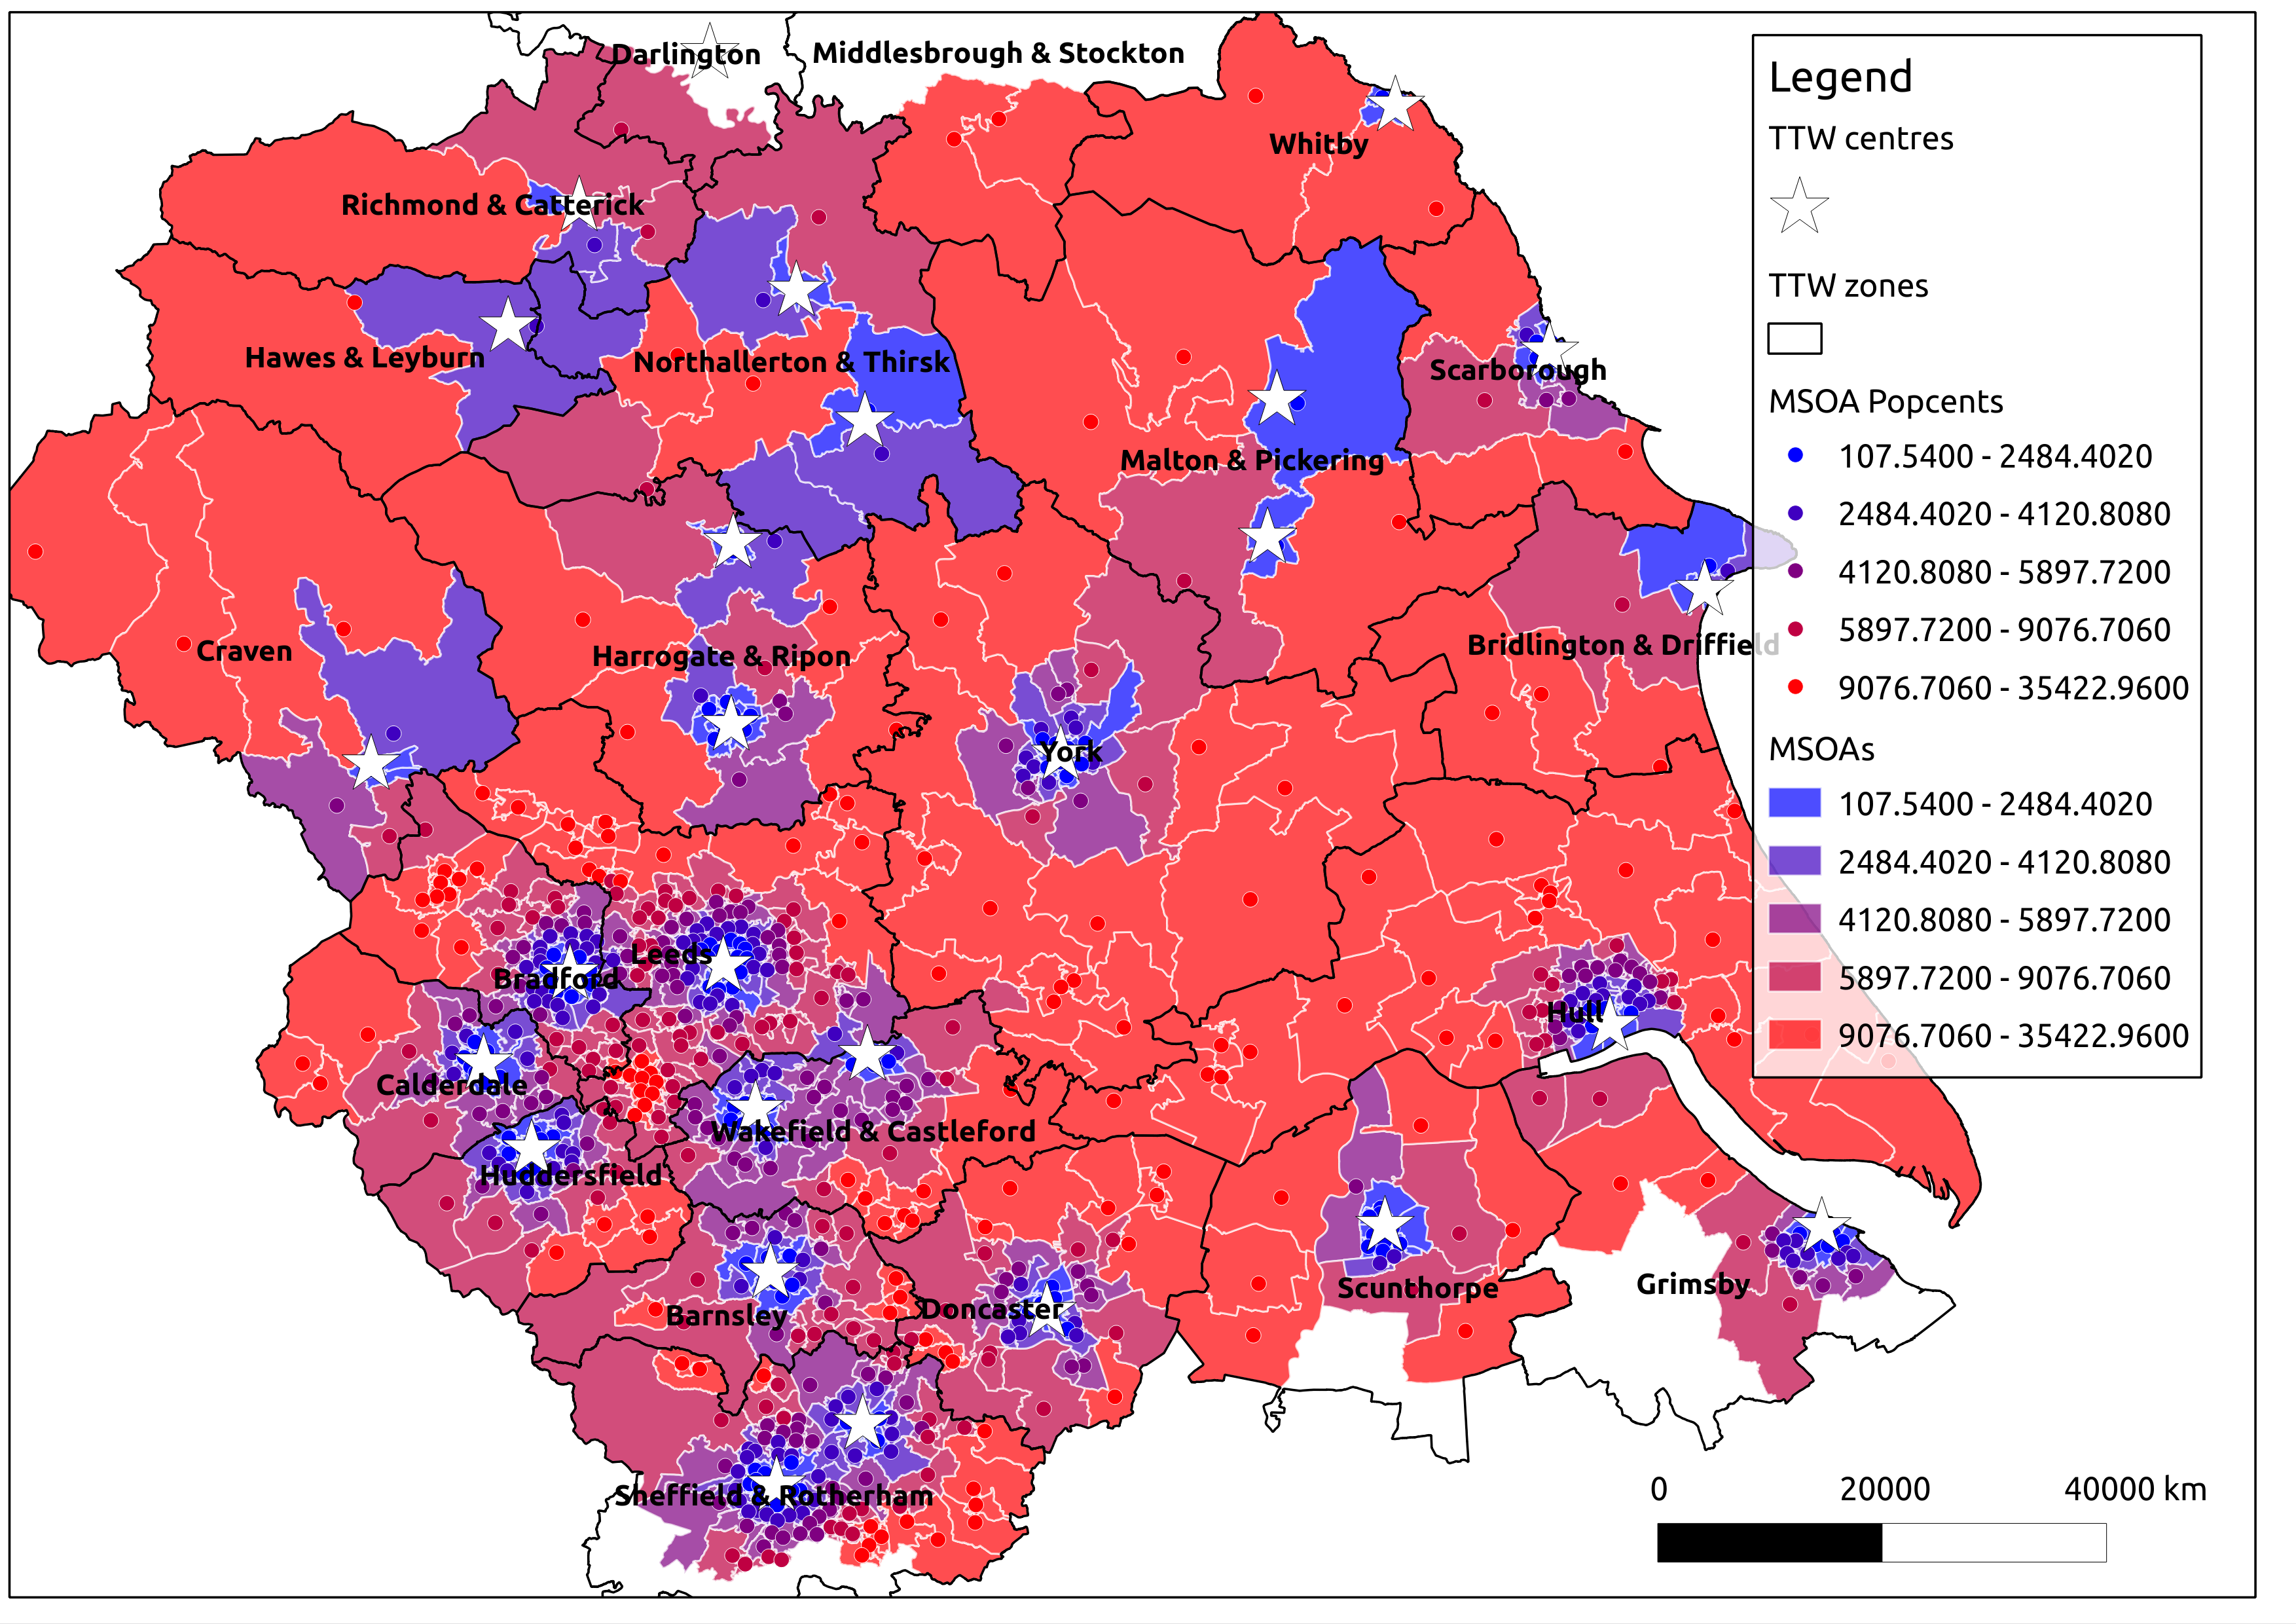
\includegraphics[width=16 cm]{dist-TTW-cent.png}\end{center}
 % cc-trans.png: 1113x529 pixel, 72dpi, 39.26x18.66 cm, bb=0 0 1113 529
 \caption{Illustration of how distance to employment centre was calculated.}
 \label{fig:dist-ttw-cent}
\end{figure}

% !!! Something here about the link between remoteness, rurality and IMD. !!!

\section{Building a spatial microsimulation model in R} \label{setsim}
The previous sections have established the availability of high quality data
on commuting behaviour at geographic and individual levels. Associated
variables such as remoteness and proximity to key transport networks and nodes
can also be inferred based on good geographic data. The challenge now from a
modelling perspective is to join all these elements together.
% Yes but you have not explained how topography/remoteness is included via msim
% methods!!!
Travel to work is
clearly an activity that occurs at the individual level. Overall patterns of
commuting can be expected to be closely related to larger scale processes ---
such as the nature of labour and housing markets, cultural norms and the main
sectors of local economic activity. However, commuting \emph{behaviour} is
always undertaken by individuals making decisions over which they have
some degree of control. %%%!!! Something about agency-structure here?
From short-term choices about at what time to get into work (increasingly
common due to `flexi-time') to strategic decisions about where to live and
work, individuals influence their commuting patterns.

The critical next step, therefore, is to generate spatial microdata on
commuting: individual level data allocated to spatial areas. This is where
spatial microsimulation comes in, to combine the aggregate level commuting
data with the individual level data presented in the previous section.
The technique used in this thesis is Iterative Proportional Fitting (IPF), which
is described in \cref{Chapter3}. The IPF algorithm allocates a weight to each
individual for each area under consideration. If the individual is highly
representative of the area (relative to the individual level dataset) the
weight will increase; if the individual is not representative of the area in
question (or is not present), the weight will decrease.  

As discussed in \cref{Chapter3}, computer hardware has long influenced, and even
\emph{determined} the types of analysis that can be conducted at the individual
level. Hardware limitations are far less of a constraint than they used to be,
elevating the importance of software. As \citet{Holm1987} made clear more than
20 years ago,
% in a section entitled `programming languages',
the choice of software also
has a major impact on the model's flexibility, efficiency, reproducibility and
ease of coding. It was noted that ``little attention is paid to the
choice of programming language used'' \citep[p.~153]{Holm1987}, an observation
that appears to be as true now as it was then. % Search for languages? no.???
For this research, a conscious decision was made early on to use R, and this
has had an impact on the model construction, features, analysis and even design
philosophy. It is at this stage, therefore, that R as a platform for undertaking
spatial microsimulation is discussed in some detail. The theory is discussed in
\cref{s:theory}

\subsection{Why R?}
The majority of the quantitative analysis conducted for this thesis, and the
entirety of the spatial microsimulation model used, was written in R. This was
a deliberate choice made at the outset rather than an arbitrary decision based
on predecessors. This section briefly explains the importance of choosing
appropriate computer software in academic research in general, with respect to
reproducibility, a cornerstone of science. The choice of R in particular is then
described. R was chosen for its virtues, which are summarised well in
\citet{Matloff-R}:

\begin{itemize}
\item ``a public-domain implementation of the widely-regarded S statistical
language; R/S is the de facto standard among professional statisticians
\item comparable, and often superior, in power to commercial products in most
senses
\item available for Windows, Macs, Linux
\item in addition to enabling statistical operations, it's a general programming
language, so that you can
automate your analyses and create new functions
\item object-oriented and functional programming structure
\item your data sets are saved between sessions, so you don't have to reload
each time
\item open-software nature means it’s easy to get help from the user
community''
\end{itemize}

\citet{Matloff-R} also provides five
examples of the type of people who would be interested in programming in R,
rather than using it as a quick and easy tool for graphing and numerical
analysis. Of particular relevance to this thesis is the second of Matloff's 
categories of people for whom R is recommended:
``Academic researchers developing statistical methodology that is either new or
combines existing methods into an integrated procedure that needs to be codified
for usage by the general research community'' \citep[p.~xiii]{Matloff-R}.

The quote also suggests some of the potential advantages of writing multi-use
scripts in R rather than a collection of unrelated functions: by its
very nature modelling is an iterative exercise, so it is important to be able
to invoke specific chunks of code (e.g.~using the \verb source() ~command) that
are modular. While this capability is not unique to R, the range of statistical functions that
can be performed within a unified environment is. The
rapidly growing use of R for spatial data analysis was another factor that
makes it well-suited to spatial-microsimulation and other types of geographic
modelling (e.g.~\citealp{Singleton2013-school}). R overcomes the need to switch
between several different programs (e.g.~one for analysis, one for graphing,
one for mapping), increasing simplicity and (eventually) productivity.

Despite all these advantages, R has a number of weaknesses itemised below along with techniques and projects which mitigate them:
\begin{itemize}
 \item R loads everything into RAM. This can be problematic when querying
 large datasets, of which only one part needs to be accessed at a
 time.\footnote{ This is especially common with geographical analysis, which often focus
 on a small area of a large map at a time \citep{Obe2011}.
 }
 There are numerous tools
 that overcome this constraint by querying databases (stored on the hard-disk) from within R, including
 RMySQL \citep{james2012rmysql} and Rattle \citep{Williams2009}. \citet{Singleton2013-school}
 queried a PostGIS database from within R to estimate the route taken by school
 commuters, for the estimation of associated CO$_2$ emissions.
 \item R can be slow, for example running for loops and when used as a general programming
 language which is not R’s main purpose. R being an
 interpreted language there are times when the performance advantages of a compiled language such as 
 C/C++ are needed.
 To this end the RCPP package was developed, which provides
 ``Seamless R and C++ integration''  \citep{eddelbuettel2011rcpp}. Packages are also available
 to integrate R with Java (rJava), Python (rpy2) and text markup languages such as Markdown and
 \LaTeX (knitr). Also, the base installation of R provides an inbuilt C compiler for doing the
 `heavy lifting' tasks such as kernel density estimation \citep{peng2002introduction}.
 These links to other languages could be useful for porting pre-existing algorithms
 for spatial microsimulation into R (e.g.~\citealp{Williamson2007, Ballas2007simb}).
 \item R's base graphics are unattractive and unintuitive. This problem has been
 tackled most comprehensively in a PhD thesis by Hadley Wickham \citep{Wickham2008}.
 The aim was to implement the `grammar of graphics' \citep{wilkinson2005grammar},
 a comprehensive and coherent approach to data visualisation, into an existing
 open-source statistical programming language. The result is ggplot2,
 which has a very active user and developer community \citep{wickham2011ggplot2}.
 ggplot2 has been used throughout this thesis for plotting with help from key
 references \citep{wickham2011ggplot2, chang2012r}.
 \item R's visualisations are not dynamic. This problem has been partly
 overcome in the realm  of GIS with two QGIS plugins: ManageR and Home range.
 For dynamic web applications, the R package Shiny provides similar interactive
 functionality as Google's Fusion tables project. There is also a nascent
 interface between R and Processing (rprocessing), an abstraction of Java
 ideal for dynamic
 visualisations of geographic data (e.g.~\citealp{wood2010visualisation}).
\end{itemize}


\subsection{IPF theory: a worked example} \label{s:theory}
In most modelling texts there is a strong precedence of theory over
application: the latter usually flows from the former. The location 
of this section after a description of the programming language
R is therefore a little unconventional but there is a logic to this order. 
Having demonstrated the power and flexibility of the programming language in
which the model is written, the next stage is to analyse the task to which it
is to be set. More importantly for reproducible research, this theory section
is illustrated with a simple worked example that culminates in
a question to the reader, to test his or her understanding.

IPF is a simple statistical procedure, ``in which cell counts in a contingency
table containing the sample observations are scaled to be consistent with
various externally given population marginals'' \citep{mcfadden2006testing}. In
other words, and in the context of \emph{spatial} microsimulation, IPF produces
maximum likelihood estimates for the frequency with which people appear in
different areas. The method is also known as `matrix raking' or the RAS
algorithm, (\citealp{Birkin1988, Muller2010,
Simpson2005, Kalantari2008, Jirousek1995}) and has been described as one
particular instance of a more general procedure of `entropy maximisation'
\citep{Johnston1993, blien1998entropy}.
The mathematical properties of IPF
have been described in several papers
(\citealp{Bishop1975, Fienberg1970, Birkin1988}).
Illustrative examples of the procedure can be found in
\citet{Saito1992}, \citet{Wong1992}
and \citet{Norman1999a}. \citet{Wong1992} investigated the reliability of IPF
and evaluated the importance of different factors influencing the its
performance. Similar methodologies have since been employed by
\citet{Mitchell2000}, \citet{Williamson2002} and
Ballas et al.~\citeyearpar{Ballas2005c, Ballas2005}
to investigate a wide range of phenomena.

% As \citet{Birkin1988} point out, IPF undertakes the basic task of
% generating a vector of individual characteristics, $x = (x_1, x_2, ..., x_m)$ on the
% basis of a joint probability distribution $p(x)$. Once the probability distribution
% for such a vector is generated, representative
% individuals can be synthesised or extracted from a pre-existing survey dataset.
% However, when information is not available for the full joint distribution, there
% is a need to construct a product of conditional and marginal probabilities,
% by building one attribute at a time, so that the probability of certain attributes
% is conditionally dependent on existing attributes \citep{Birkin1988}:
%
% \begin{equation}
% p(x) = p(x_1)p\left( \frac{x_2}{x_1}\right) p\left( \frac{x_3}{x_2}, x_1\right) \times
%  ... \times p\left( \frac{x_m}{x_{m-1}},...,x_1\right)
% \end{equation}
%
% IPF can be used to model the joint probability distribution
% $p(x_1, x_2, x_3)$ subject to known probabilities
% $p(x_1, x_2)$ and $p(x_1, x_3)$. Following \citet{Birkin1988} and \citet{Ballas2007simb},
% if $p(x_1, x_2, x_3)$ is the $i^{th}$ approximation to the three-attribute joint probability
% vector then:
% \begin{equation}
%  p^1(x_1, x_2, x_3) = \frac{1}{N_1 N_2 N_3}
% \end{equation}
% where $N_j$ is the number of possible states associated with the attribute vector $x$.
% The vector can then be adjusted in \emph{proportion} to the following known constraints:
% \begin{equation}
% p^2(x_1, x_2, x_3) = p^1(x_1, x_2, x_3) \frac{p(x_1, x_2)}
% {{\displaystyle \sum^{}_{x_3}{p^1(x_1, x_2, x_3)}}}
% \label{eq:p2}
% \end{equation}
% \begin{equation}
% p^3(x_1, x_2, x_3) = p^2(x_1, x_2, x_3) \frac{p(x_1, x_3)}
% {{\displaystyle \sum^{}_{x_2}{p^1(x_1, x_2, x_3)}}}
% \label{eq:p3}
% \end{equation}
% IPF involves iterating through equations \ref{eq:p2} and \ref{eq:p3}
% until a \emph{fitted} distribution is obtained, when the probabilities
% are convergent within some acceptable limit \citep{Birkin1988, Fienberg1970, Ballas2007simb}.
% This procedure can be generalised to a larger number of attributes \citep{Birkin1988}:
% if we let $Z_k(x)$ be a subset of the set of attribute vectors
% $E(x)$ for which marginal joint probabilities are known and let $W_k(x)$ be
% the complement of $Z_k(x)$, that is $W_k(x)= E(x) - Z_k(x)$, then:
%
% \begin{equation}
%  p^1(x) = \frac{1}{\displaystyle{\prod^{m}_{i=1}{Ni}}}
% \end{equation}
% \begin{equation}
%  p^2(x) =  p^1(x) \frac{p[Z_1(x)]}{\displaystyle{\sum^{}_{W_1(x)}{p^1(x)}}}
% \label{eq:six}
% \end{equation}
%
% {\centering
% .
%
% .
%
% .
%
% }
%
% \begin{equation}
%  p^{k+1}(x) =  p^k(x) \frac{p[Z_k(x)]}{\displaystyle{\sum^{}_{W_k(x)}{p^k(x)}}}
% \label{eq:seven}
% \end{equation}
%
% IPF iterates through equations \ref{eq:six} and \ref{eq:seven} until convergence
% \citep{Birkin1988}. An extensive discussion of the mathematical properties of
% IPF can be found in \citet{Fienberg1970}.

To illustrate how IPF works in practice, a simplified example is described below.
This is a modified version of a simpler demonstration from
\citet{Ballas2005}.\footnote{In \citet{Ballas2005}
the interaction between the age and sex constraints are assumed to be known.
(Their equivalent of \cref{t:s2} contains data for every cell,
not question marks.) This results in IPF converging instantly.
However, in Census data, such cross-tabulation is
often absent, and IPF must converge over multiple constraints and
iterations. This latter scenario is assumed in the worked example below. Other
worked examples of the principles are provided in \citet[Appendix
3]{johnston1985geography} (for entropy maximisation), \citet{Norman1999a} and
\citet{Simpson2005} (using the proprietary statistical software SPSS).
}
Table \ref{t:w}  describes a
hypothetical microdataset comprising 5 individuals, who are defined by two
constraint variables, age and sex. Each has two categories.
Table \ref{t:s} contains aggregated data
for a hypothetical area, as it would be downloaded from census dissemination
portal Casweb. \Cref{t:s2} illustrates this table in a different form,
which shows our ignorance of interaction between age and sex.


\begin{table}[h]
\centering
\caption[A hypothetical input microdata set]{A
hypothetical input microdata set (the original
weights set to one). The bold value is used subsequently for
illustrative purposes.}
\begin{tabular}{llll}
\toprule
{Individual } & {Sex} & {Age-group} & {Weight} \\
\midrule
1 & Male & Over-50 & 1 \\
2 & Male & Over-50 & 1 \\
3 & {Male} & {Under-50} & \textbf{1} \\
4 & Female & Over-50 & 1 \\
5 & Female & Under-50 & 1 \\
\bottomrule
\end{tabular}
\label{t:w}
\end{table}
\vspace{1cm}


\begin{table}[htbp]
\centering
\caption{Hypothetical small area constraints data ($s$).}
\begin{tabular}{cllll}
\toprule
Constraint $\Rightarrow$ & \multicolumn{2}{c}{$i$}& \multicolumn{2}{c}{$j$}\\
Category $\Rightarrow$ & $i_1$ & $i_2$ & $j_1$ & $j_2$ \\
Area $\Downarrow$  & Under-50 & Over-50 &  Male & Female\\
1  & 8 & 4 & 6 & 6\\
\bottomrule
\end{tabular}
\label{t:s}
\end{table}
\vspace{1cm}

\begin{table}[htbp]
\centering
\caption[Small area constraints expressed as marginal totals]{Small
area constraints expressed as marginal totals, and the cell
values to be estimated.}
\begin{tabular}{cllll}\toprule
Marginal totals&  & \multicolumn{2}{c}{$j$} & \\
& Age/sex & Male & Female & T\\ \midrule
\multirow{2}{*}{$i$} & Under-50 & \textbf{?} & ? & 8\\
& Over-50 & ? & ? &4 \\
& T & 6 & 6 &12\\
\bottomrule
\end{tabular}
\label{t:s2}
\end{table}

Table \ref{t:m} presents the
hypothetical microdata in aggregated form,
that can be compared directly to Table \ref{t:s2}.

\begin{table}[htbp]
\centering
\caption[The aggregated results of the weighted
microdata set]{The aggregated results of the weighted
microdata set ($m(1)$).
Note, these values depend on the
weights allocated in Table \ref{t:w} and therefore
 change after each iteration}

\begin{tabular}{cllll}\toprule
Marginal totals&  & \multicolumn{2}{c}{$j$} & \\
& Age/sex & Male & Female & T\\ \midrule
\multirow{2}{*}{$i$} & Under-50 & \textbf{1} & 1 & 2\\
& Over-50 & 2 & 1 &3 \\
& T & 3 & 2 &5\\
\bottomrule
\end{tabular}
\label{t:m}
\end{table}

Using these data it is possible to readjust the weights of the hypothetical
individuals, so that their sum would add up to the totals given in Table
\ref{t:s2} (12). In particular, the weights can be readjusted by multiplying them by
the marginal totals, originally taken from
Table \ref{t:s} and then divided by the respective marginal total in \ref{t:m}.
Because the total for each small-area constraint is 12, this must be
done one constraint at a time. This
can be expressed, for a given area and a given constraint ($i$
or age in this case), as follows:

\begin{equation}
w(n+1)_{ij} = \frac{w(n)_{ij} \times sT_{i}}{mT(n)_{i}}
\label{eq:ipf}
\end{equation}
where $w(n+1)_{ij}$ is the new weight for individuals with characteristics $i$
(age, in this case), and $j$ (sex),  $w(n)_{ij}$ is the original
weight for individuals with these characteristics, $sT_{i}$ is element
marginal total of the small area constraint, $s$
(Table \ref{t:s}) and $mT(n)_{i}$ is the marginal total of category
$j$ of the aggregated results of the weighted
microdata, $m$ (Table \ref{t:m}). $n$ represents the iteration number.
Although the marginal totals of $s$ are known, its cell values
are unknown. Thus, IPF estimates the interaction (or cross-tabulation)
between constraint variables.
(Follow the emboldened values in the tables
to see how the new weight of individual 3 is calculated for the sex constraint.)
Table \ref{t:new-weights} illustrates the weights that result. Notice that the
sum of the weights is equal to the total population, from the constraint variables.

\begin{table}[htbp]
\centering
\caption{Reweighting the hypothetical microdataset in order to fit
Table \ref{t:s}.}
\begin{tabular}{lllll}
\toprule
{Individual} & {Sex} & {age-group} & {Weight} &
{New weight, w(2)} \\ \midrule
1 & Male & Over-50 & 1 & $1 \times 4/3 = \frac{4}{3}$ \\
2 & Male & Over-50 & 1 & $1 \times 4/3 = \frac{4}{3}$ \\
3 & Male & Under-50 & 1 & $\textbf{1} \times
\textbf{8}/\textbf{2} = 4$ \\
4 & Female & Over-50 & 1 & $1 \times 4/3 = \frac{4}{3}$ \\
5 & Female & Under-50 & 1 & $1 \times 8/2 = 4$ \\
\bottomrule
\end{tabular}
\label{t:new-weights}
\end{table}

After the individual level data have been re-aggregated (\cref{t:m2}),
the next stage is to repeat \cref{eq:ipf} for the age constraint to generate a
third set of weights, by replacing
the $i$ in $sT_{i}$ and $mT(n)_{i}$ with $j$ and incrementing the value of n:

\begin{equation}
w(3)_{ij} = \frac{w(2)_{ij} \times sT_{j}}{mT(2)_{j}}
\label{eq:ipf2}
\end{equation}

To test your understanding of IPF, apply \cref{eq:ipf2} to the information above
and that presented in \cref{t:m2}.
This should result in the following vector of new weights, for individuals 1 to 5:
\begin{equation}
%  w(3) = (\frac{6}{5}, \frac{?}{?}, \frac{18}{5}, \frac{?}{?}, \frac{9}{2})
  w(3) = (\frac{6}{5}, \frac{6}{5}, \frac{18}{5}, \frac{3}{2}, \frac{9}{2})
\end{equation}
As before, the sum of the weights is equal to the population of the area (12).
Notice also that after each iteration the fit between the marginal
totals of $m$ and $s$
improves. The total absolute error (TAE, see \cref{etae} below)
from $m(1)$ to $m(2)$ improves from
14 to 6 in \cref{t:m} and \cref{t:m2} above. TAE for $m(3)$ (not shown,
but calculated by aggregating $w(3)$) improves even more, to 1.3.
This number would eventually converge to 0 through subsequent
iterations, as there are no empty cells in the input microdataset;
a defining feature of IPF.


\begin{table}[htbp]
\centering
\caption[Aggregated results after constraining for age]{The
aggregated results of the weighted
microdata set after constraining for age ($m(2)$).
}

\begin{tabular}{cllll}\toprule
Marginal totals&  & \multicolumn{2}{c}{$i$} & \\
& Age/sex & Male & Female & T\\ \midrule
\multirow{2}{*}{$j$} & Under-50 & 4 & 4 & 8\\
& Over-50 & $\frac{8}{3}$ & $\frac{4}{3}$ & 4 \\
& T & $6\frac{2}{3}$ & 5$\frac{1}{3}$ & 12\\
\bottomrule
\end{tabular}
\label{t:m2}
\end{table}

The above process, when applied to more categories (e.g. socio-economic class)
and repeated iteratively until a satisfactory convergence occurs, results in a
series of weighted microdatasets, one for each of the small areas being
simulated. This allows for the estimation of variables whose values are not
known at the local level (e.g. income) \citep{Ballas2005}. An issue
with the results of IPF (absent from combinatorial optimisation methods),
however, is that it results in non-integer weights: fractions of individuals
appear in simulated areas. As described in the introduction, this is not ideal
for certain applications. Integer weights allow the results of spatial
microsimulation to be further processed using dynamic microsimulation and agent
based modelling techniques \citep{Pritchard2012}.


% A key benefit from a policy perspective is that
% IPF and other spatial microsimultion techniques
% can provide estimation of variables whose values are not
% known at the local level (e.g. income).
Spatial microsimulation can also provide insight into the likely
distribution of individual level variables about which only
geographically aggregated statistics have been made available.
An issue
with the results of IPF (absent from combinatorial optimisation methods),
however, is that it results in non-integer weights: fractions of individuals
appear in simulated areas.

\subsection{Implementing IPF in R} \label{simplementing}
The above example is best undertaken by hand, probably with a pen and paper
to gain an understanding of IPF, before the process is automated for 
larger datasets. This section explains how the IPF
algorithm described above was implemented in R, using a slightly more
complex example.
% This section is based on ``Spatial microsimulation in R: a
% beginner’s guide to iterative proportional fitting (IPF)'', a tutorial
% written to accompany a methods paper on integerisation
\citep{Lovelace2013-trs}.\footnote{This tutorial is available from Rpubs, a site dedicated
to publishing R analyses that are reproducible. It uses the RMarkdown
mark-up language, which enables R code to be run and presented within
documents. See http://rpubs.com/RobinLovelace/5089 \label{fnrpub} .}

\emph{Loading in the data}

In the full model the input datasets are stored as .csv files, one for each
constraint and one for the input microdata, and read in with the command
\verb read.csv . For the purposes of understanding how the model works,
the dataset is read line by line, following the
example above. The following code creates example datasets,
based on the same hypothetical survey of 5 individuals described above,
and 5 small areas. The spatial microsimulation model will select individuals
based on age and sex and mode of transport (mode of transport
is also used on the larger online example described in footnote \ref{fnrpub}).
For consistency with the (larger) model used for the paper, 
the individual level data will be referred to as USd (Understanding Society dataset)
and the geographic data as all.msim (for all constraint variables).
The code to read-in the individual level data are presented in code sample \ref{cusd}.
When called, the data are then displayed as a table (see listing \ref{cout}).
\begin{lstlisting}[float=h, caption={Manual input of individual level data
in R}, label=cusd]
# Read in the data in long form (normaly read.table() used)
c.names <- c("id", "age", "sex")
USd <- c(       1, 59, "m",
                2, 54, "m",
                3, 35, "m",
                4, 73, "f",
                5, 49, "f")
USd <- matrix(USd, nrow = 5, byrow = T) # Long data into matrix
USd <- data.frame(USd) # Convert this into a dataframe
names(USd) <- c.names # Add correct column names
USd$age <- as.numeric(levels(USd$age)[USd$age]) # Age is a numeric
\end{lstlisting}
\begin{lstlisting}[float=h, caption={Output of the USd data frame}, label=cout]
USd # Show the data frame in R
##   id age sex
## 1  1  59   m
## 2  2  54   m
## 3  3  35   m
## 4  4  73   f
## 5  5  49   f
\end{lstlisting}
The same procedure applies to the geographical data (listing \ref{cgeo}).
\begin{lstlisting}[float=h*, caption={Geographic data input}, label=cgeo]
 category.labels <- c("16-49", "50+" # Age constraint
             ,"m", "f" # Sex constraint
             # more constraints could go here
             )
all.msim <- c(  8, 4,    6, 6,   # Original aggregate data
                2, 8,    4, 6,   # Elderly
                7, 4,    3, 8,   # Female dominated
                5, 4,    7, 2,   # Male dominated
                7, 3,    6, 4    # Young
                )
all.msim <- matrix(all.msim, nrow = 5, byrow = T) 
all.msim <- data.frame(all.msim) # Convert to dataframe
names(all.msim) <- category.labels # Add correct column names
\end{lstlisting}

IPF relies on the assumption that all constraint variables will contain the
same number of people. This is logical (how can there be more people classified
by age than by sex?) but can cause problems for constraint variables that use
only a subset of the total population, such as those who responded to questions on
travel to work. To overcome this problem, it is possible to normalise the
constraint variables, setting the total for each to the one that has the most
reliable total population. This worked example simply checks whether
or not they are (listing \ref{ccheck}).

\begin{lstlisting}[float=h, caption={R code to check the constrain populations
match}, label=ccheck]
 # Check totals for each constraint match
rowSums(all.msim[,1:2]) # Age constraint
## [1] 12 10 11  9 10
rowSums(all.msim[,3:4]) # Sex constraint
## [1] 12 10 11  9 10

rowSums(all.msim[,1:2]) == rowSums(all.msim[,3:4])
## [1] TRUE TRUE TRUE TRUE TRUE
\end{lstlisting}

\emph{Reweighting the survey dataset}

Iterative proportional fitting determines the weight allocated to each
individual for each zone to best match the geographically aggregated data.
A weight matrix is therefore created, with rows corresponding to individuals
and columns to zones, as described in \cref{s:theory}. In
R, this, and the creation of the aggregated results matrix,
is done with code presented in listing
\ref{cws}).\footnote{In subsequent
versions of the model, single, multi-dimensional weight and
aggregated result matrices are used,
to reduce the length of the scripts.
} 

\begin{lstlisting}[float=h, caption={Creating arrays of weights in R},
label=cws]
weights0 <- array(dim=c(nrow(USd),nrow(all.msim)))
weights1 <- array(dim=c(nrow(USd),nrow(all.msim)))
weights2 <- array(dim=c(nrow(USd),nrow(all.msim)))

weights0[,] <- 1 # sets initial weights to 1

USd.agg <- array(dim=c(nrow(all.msim),ncol(all.msim)))
USd.agg1 <- array(dim=c(nrow(all.msim),ncol(all.msim)))
USd.agg2 <- array(dim=c(nrow(all.msim),ncol(all.msim)))
colnames(USd.agg1) <- category.labels
\end{lstlisting}

It is important to note that in real survey data, the variables are not
always neatly categorised into the same bins as the levels of the aggregate
data. Age, for example can be classified in many different ways.
Also, a wide form is useful for subsequent steps.
Therefore, it is necessary to convert the `thin' survey dataset
into a wider form, by converting a single column such as age or sex into
multiple columns corresponding to the number of categories. Sometimes the
cut-off points of the categories can be decided (as with age), or categories
can be merged (when many different NA options are available, for example).
The code that performs this important process for our example dataset is
presented in listing \ref{ccat}.

\begin{lstlisting}[float = h, caption={R code to convert the survey
dataset into binary form}, label=ccat]
USd.cat <- array(rep(0), dim=c(nrow(USd),
			  length(category.labels !=0)))

USd.cat[which(USd$age < 50),1] <- 1 # Age, "< 50"
USd.cat[which(USd$age >= 50),2] <- 1 # "50+"
USd.cat[which(USd$sex =="m"),3] <- 1 # Sex constraint: "m"
USd.cat[which(USd$sex =="f"),4] <- 1 #"f"
sum(USd.cat) # Should be 10
\end{lstlisting}

Another important step shown in \cref{s:theory} was that of converting the
`long' survey dataset into a form that can be compared directly with the
aggregated constraint variables. Listing \ref{cconv} shows how this is done
in R, and the code needed to view the results. (Notice that the first row
of all.msim is the same as those displayed in \cref{t:s})

\begin{lstlisting}[float=h, caption={R code to aggregate the survey dataset},
label=cconv]
 for (i in 1:nrow(all.msim)){ # Loop creating aggregate values 
  USd.agg[i,]   <- colSums(USd.cat * weights0[,i])
}

# Test results
USd.agg

##      [,1] [,2] [,3] [,4]
## [1,]    2    3    3    2
## [2,]    2    3    3    2
## [3,]    2    3    3    2
## [4,]    2    3    3    2
## [5,]    2    3    3    2

all.msim

##   16-49 50+ m f
## 1     8   4 6 6
## 2     2   8 4 6
## 3     7   4 3 8
## 4     5   4 7 2
## 5     7   3 6 4

plot(as.vector(as.matrix(all.msim)),
  as.vector(as.matrix(USd.agg)), xlab = "Constraints",
    ylab = "Model output")
abline(a = 0, b = 1)
\end{lstlisting}

With the data loaded and processed into comparable formats, one is in a
position to start comparing how well our individual level survey dataset
fits with the aggregate constraints (see listing \ref{cconv}). Note that for USd.agg,
the results are the same for every zone, as each individual has a weight of 1
for every zone. Note also the very poor fit between the variables at the
aggregate level, as illustrated by poor correlation between the constraint and
microdata variables (r = 0.05), and a plot of the fit presented in \cref{fct1}.
The next stage is to apply the first constraint,
to adjust the weights of each individual so they match the age constraints
(listing \ref{ccon1} --- note that the top row USd.agg1 is the same as
\cref{t:m2}). After this operation, the fit between the constraint
variables and the aggregated microdata are far better (r = 0.67), but there
is still a large degree of error (\cref{fc1}).

\begin{figure}[h]
 \begin{center}
   
\includegraphics[width = 10cm]{unnamed-chunk-5}
 \end{center}
\caption[Scatter plot of the fit between census and survey data]
{Scatter plot of the fit between census and survey data. This plot
can be re-created using the plot command in listing \ref{cconv}.}
 \label{fct1}
\end{figure}

\begin{lstlisting}[float=h, caption={Reweighting of first constraint
and testing of results}, label=ccon1]
for (j in 1:nrow(all.msim)) {
 weights1[which(USd$age < 50),j] <- all.msim[j,1]/USd.agg[j,1]
 weights1[which(USd$age >= 50),j] <- all.msim[j,2]/USd.agg[j,2]
}
# Aggregate the results for each zone
for (i in 1:nrow(all.msim)) {
 USd.agg1[i,] <- colSums(USd.cat * weights0[,i] * weights1[,i])
}
# Test results
USd.agg1
##      16-49 50+     m     f
## [1,]     8   4 6.667 5.333
## [2,]     2   8 6.333 3.667
## [3,]     7   4 6.167 4.833
## [4,]     5   4 5.167 3.833
## [5,]     7   3 5.500 4.500

plot(as.vector(as.matrix(all.msim)),
 as.vector(as.matrix(USd.agg1)), xlab = "Constraints",
 ylab = "Model output")
abline(a = 0, b = 1)
\end{lstlisting}

\begin{figure}[h]
 \begin{center}
  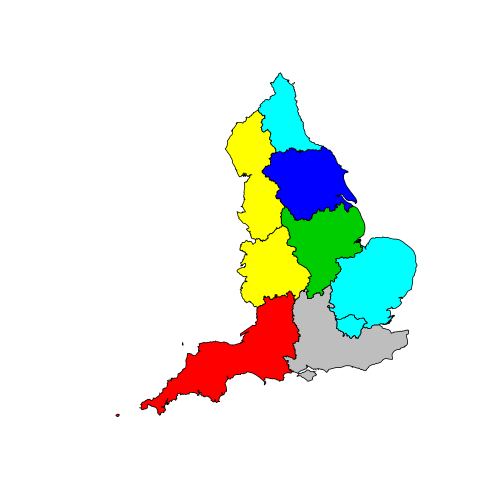
\includegraphics[width=10cm]{unnamed-chunk-6}
 \end{center}
\caption{Scatter plot showing the fit after constraining by age.} \label{fc1}
\end{figure}

We will perform the same checks after
each constraint to ensure our model is improving.
To see how the weights change for each individual for each area,
one simply types \verb weights1 , for constraint 1 (listing \ref{cmat}).
Note that the first column of weights 1 is the same as \cref{t:s}.
\begin{lstlisting}[caption = {The new weight matrix. Previously all weights were set to one.},
label =cmat]

##       [,1]  [,2]  [,3]  [,4] [,5]
## [1,] 1.333 2.667 1.333 1.333  1.0
## [2,] 1.333 2.667 1.333 1.333  1.0
## [3,] 4.000 1.000 3.500 2.500  3.5
## [4,] 1.333 2.667 1.333 1.333  1.0
## [5,] 4.000 1.000 3.500 2.500  3.5
\end{lstlisting}

To further improve the fit, one next constrains by the second aggregate constraint:
sex (listing \ref{con2}). To check that our implementation in R produces the
same results as the hand-calculated example, the resulting weights where queried.
As shown by \verb weights3[,1] , these are the same as
those calculated for $w(3)$ above.

\begin{lstlisting}[float=h, caption={Code to constrain the weights by
sex}, label=con2]
for (j in 1:nrow(all.msim)) {
    weights2[which(USd$sex == "m"),j] <-
		  all.msim[j,3]/USd.agg1[j,3]
    weights2[which(USd$sex == "f"),j] <-
		  all.msim[j,4]/USd.agg1[j,4]
}

weights3 <- weights0 * weights1 * weights2
for (i in 1:nrow(all.msim)) {
  USd.agg2[i,] <- colSums(USd.cat * weights3[,i])
}

weights3[,1]

## [1] 1.2 1.2 3.6 1.5 4.5
\end{lstlisting}

The model fit improves greatly after constraining for sex (r = 0.992).
However, to ensure perfect fit more iterations are needed. Iterating
just once more, as done on the online version of this
section\footnote{See
\href{http://rpubs.com/RobinLovelace/6193}{rpubs.com/RobinLovelace/6193}
}
results in a fit that is virtually perfect (\cref{fexits}). More iterations
are needed for larger datasets with more constraints to converge.

\begin{figure} \begin{center}
 
\includegraphics[width = 6cm]{unnamed-chunk-8}
 
\includegraphics[width = 6cm]{unnamed-chunk-11}
 \end{center}
 \caption[Improvement of model fit with iterations]
 {Improvement of model fit after constraining by sex (left)
 and after two complete iterations (right).} \label{fexits}
\end{figure}

The worked code example in this section is replicable.
If all the code snippets are entered, in order, the results
should be the same on any computer running R. There
is great scope for taking the analysis further:
some further tests and plots are presented on the on-line
versions of this section. The simplest case is contained in
Rpubs document \href{http://rpubs.com/RobinLovelace/6193}{6193} and a more
complex case (with three constraints) can be found in Rpubs document
\href{http://rpubs.com/RobinLovelace/5089}{5089}. The preliminary checks
done on this code are important to ensure the model is understood
at all times and is working correctly. More systematic methods
for model checking are the topic of the following section.

\section{Model checking and validation} \label{smeval}

The R scripts that implement the methods described in \cref{setsim} and
\cref{s:integerisation} contain over 1000 lines of code.
This means that making mistakes while writing the code was almost inevitable,
from time to
time.\footnote{
A couple of examples serve to illustrate this point: during the construction of
vulnerability metrics based on the individual level output from the spatial
microsimulation model, the estimated expenditure on commuting was divided
by equivalised household income (a proxy of disposable income). 
One issue was that trip cost estimates are per year
while the income estimates are supplied per month in the USd. It took several
more alterations and runs of the model before the cause of the high proportion
of income spent on commuting (sometimes over 100\%) was realised. Another
example is simple typing errors while writing the code. The results are
presented in \cref{fig:error}, and are described below.
}
The large size of
the output files (approximately 250 Mb for 10 iterations of the spatial
microsimulation model for Yorkshire and the Humber) means that it would
be easy to miss fundamental errors. Hence the need for a
systematic strategy of checking the output. Beyond checking the model's
internal validity, it is necessary to test its external validity. This process,
validation, is inherently limited by lack of real spatial microdata.
Validation is a crucial step to take before the results are
presented, discussed and used as the basis of policy guidance. To make an
analogy with corporate food safety standards, it is important be open about and
highlight times when things do go wrong, in order to achieve high standards
\citep{Powell2011}. Transparency is needed in modelling for similar reasons
\citep{Tamminga2012}. This section is therefore an overview of the methods used
to find fault in the model, rather than assuming that everything is working
perfectly as the rest of the thesis does. It is divided into two halves: first
the process
of comparing the model results with knowledge of how it \emph{should}
perform \emph{a-priori} (model checking). Second, the
internally consistent model results are compared with external
empirical data (validation).
Validation is also discussed in the context of a single case study
in \cref{s:valid}.

\subsection{Model checking}
A proven method of checking that data analysis and processing is working
is wide ranging and continual visual exploration of its output
\citep{janert2010data}.
This strategy has been employed
throughout the modelling process, both to gain a better understanding of the
behaviour of the underlying R code, and to search for unexpected
results. These were often precursors to error identification.

An example of this, that illustrates the utility of ad-hock checks, is the
continual plotting of model inputs and outputs to ensure that they
make sense. The R commands \verb summary() \ and \verb plot() \ are ideal for
this purpose. The former provides basic descriptive statistics; the latter
produces a graphical display of the object. Both are \emph{polymorphic},
meaning that command adapts depending on the type of object it has been asked
to process \citep{Matloff-R}. Thus, to check that
the number of people in each age and sex category in the input and output
dataset made sense overall, the
following command was issued, resulting in the plot illustrated in \cref{fasp}:

\begin{lstlisting}
plot(cut(USd$age, breaks=(seq(0,100,20))), USd$sex)\end{lstlisting}
% TAKEN FROM ~/Dropbox/vul-meth/etsimY

\begin{figure}[h]
 \begin{center}
   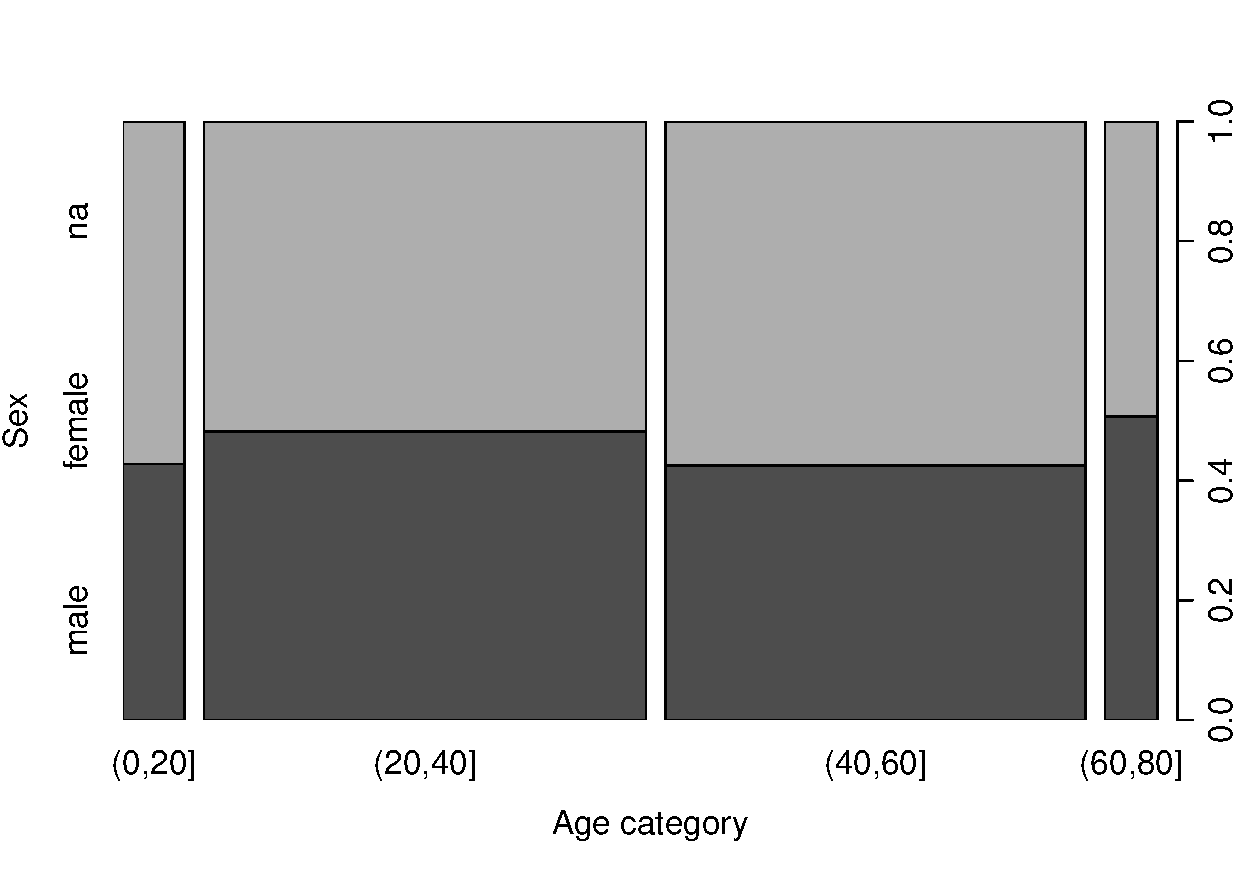
\includegraphics[width = 12cm]{age-sex-plot}
 \end{center}
 % cc-ems.pdf: 792x612 pixel, 72dpi, 27.94x21.59 cm, bb=0 0 792 612
\caption[Diagnostic plot to check the sanity of age and sex inputs.]{Diagnostic
plot to check the sanity of age and sex inputs. (Square brackets
indicate that the endpoint is not included in the set --- see
International Organization for Standardization
\href{http://www.iso.org/iso/catalogue_detail?csnumber=31887}{(ISO) 80000-2:2009},
formerly \href{http://en.wikipedia.org/wiki/Interval_(mathematics)}{ISO 31-11}
on ``mathematical signs and symbols for use in physical sciences and technology'').}
 \label{fasp}
\end{figure}
These common-sense methods of data checking may seem overly simplistic to warrant
mention. Yet such basic sanity tests are the `bread-and-butter' of
quantitative analysis. They ensure that the data are properly
understood \citep{Wickham2008}. Had the input data represented in \cref{fasp}
contained an equal proportion of people under 20 as over 20, for example,
one would know that the input data for commuters was faulty.
This approach, whereby major
problems are revealed early on in frequent tests, is preferable to waiting
until the results of the full spatial microsimulation are analysed. Hours were
saved, and understanding of the input datasets was improved.\footnote{The
use of the
same command to check model output was crucial to the identification of
important errors, including a small mistake in the code which led to large
errors in the synthetic microdata output for the distance constraint variables.}

The basic tenet of spatial microsimulation is that simulated and actual data
should match at the aggregate level \citep{Ballas2007simb}.
This knowledge led to the
continual plotting of census vs simulated results in the early stages of the
model construction, and the development of more
sophisticated plots (see \cref{fig:IPF-4c}).
Still, the humble scatter plot was used frequently for
preliminary analysis. To provide an example, after the model was run for
Yorkshire
and the Humber region for 20 iterations, I was confident the results were
correct: the results had been tested for Sheffield, and everything
\emph{seemed} to be working as expected.

Knowledge of how model-census fit should look started alarm bells
ringing when an imperfect plot was discovered:
% (largely by luck, as I was looking at the fit
% between only some of the variables, and happened to think the number of people
% taking very short trips could be subject to higher than normal levels of
% error). % What does this contribute? Nowt.
\cref{fig:error} (A) was cause for concern, not only for the low
correlation between the two variables (which was still greater than 0.8), but
because the direction of the error: the model had \emph{always} overestimated the
number of people travelling short distances to work in past runs.
This seemed suspicious, and the relationship was plotted for earlier constraints
to identify where the problem was variables were plotted.
\cref{fig:error} (B) was the
result of this, after constraining by distance.
Something had clearly gone wrong because no people who work
from home had been registered in the aggregate output. These issues led to
a re-examination of the code contained
within the file cats.r. It was found that a faulty placement of an
equals sign (such that values ``greater than or equal'' to 0 were accepted as 0
- 2 km travel to work). The problem was solved, and the model correlation
improved as a result (\cref{fig:error} (C)).

The two examples described above provided insight into how the model was
performing by its own standards. The more challenging stage is to validate
the model against factors external to it. % This is further discussed !!!

\begin{figure}[h]
  \begin{center}
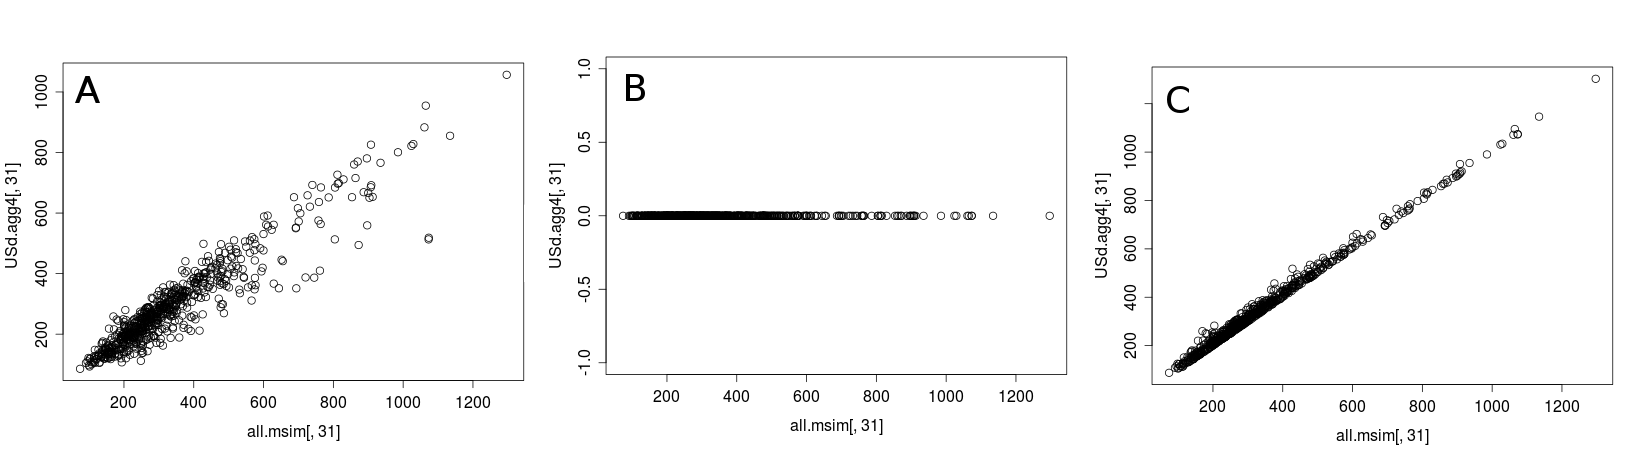
\includegraphics[width=15cm]{errors3-1}      \end{center}
 % cc-trans.png: 1113x529 pixel, 72dpi, 39.26x18.66 cm, bb=0 0 1113 529
 \caption[Diagnostic plots to identify model error]{Three diagnostic plots used
to identify a code error in the spatial microsimulation model (for the
distance category `travels 0--2 km to work'). The x-axis is
census data, the y-axis is the simulated result. A) First plot
analysed (for iteration 20); B) second plot, which illustrated the source of the
problem, in the distance constraint; C) satisfactory diagnostic plot,
after the problem had been resolved.}
 \label{fig:error}
\end{figure}

\subsection{Model validation}
\label{meval}
% {\color{red} Should this section be in a later chapter?} !!!
Beyond `typos' or simple conceptual errors in model code, more fundamental
questions should be asked of spatial microsimulation models. The validity
of the assumptions on which they are built, and the confidence one should have
in the results are important. This is especially true of models designed to inform
policies which have the potential to influence quality of life. Yet
evaluation and `validation' are
 problematic for any models that attempt to explain extensive, complex
systems such as cities or ecosystems. The urban modelling approach, of which
spatial microsimulation of commuters is a subset, has been grappling with this
problem since its infancy. Lacking a crystal ball, time-machine or settlements
on which controlled experiments can be performed, the difficulty of model evaluation can
seem intractable: ``only through time can a model be verified in any
conventional sense of the word'', by comparing the range of projected futures
with the reality of future change in hindsight \citep[p.~15]{batty1976urban}.

Why do urban models pose such a problem? Previously unknown knock-on impacts
cannot be ruled out due to the vast number of links between system
elements.\footnote{It is, of course, impossible to know how every resident of
an area interacts with every other, let alone predict the future impacts of
this interaction, even in the era of ubiquitous digital communications.
}
Rigorous real-world testing is usually impossible due to the scale of the system
and ethics involved with intervening in peoples' lives for the sake of research.
Controlled experiments cannot be performed on real settlements in the
same way that experiments can be performed in the physical sciences and, even if
two similar settlements could be found on which to apply different
interventions, there is no guarantee that all other factors will be held
constant throughout the duration of the experiment. %%% Refs!!!
% Going off on a bit of a waffle to be fair

Additional evaluation problems apply to spatial microsimulation models in
particular for a number of reasons, including:
\begin{itemize}
 \item The aggregate values of categorical `small area' constraint variables are already known from the Census, 
 so should be accurate. Checking the distribution of continuous variables such as 
 age and distance travelled to work against these crude categories is 
 problematic.\footnote{For example, if 50\% of
commuters in a particular area travel 2--5 km to work according to the Census,
does that mean that there is a normal distribution of trip distances with the
mean focussed on 3.5? Or is it more likely that there is a single large
employer located somewhere between 2 and 5 km from the bulk of houses in the
area, which accounts for the majority of these jobs and leads to a skewed
distribution of home-work distances. In every event, spatial microsimulation
will ignore such subtleties and smooth out extreme skewness by approximating the
national distance trends within each distance bin.
}
  \item Target variables are not generally known as geographic
aggregates. Therefore checking their validity for small areas is 
difficult: new surveys may be needed.
  \item Spatial microsimulation results in long lists of individuals for each
zone. With thousands of individuals in each zone and hundreds of zones, the
datasets can become large and unwieldy.
\end{itemize}

Regarding the target variables, inaccuracies can be expected because they are
determined entirely by their relationships with constraint variables. Also
it can be expected these relationships will not remain constant for all places:
perhaps in one area the number of female drivers is positively correlated to
distance travelled to work, yet there may be a different strength of
correlation, or the variables may be unrelated in another.

As mentioned above, validation of target variables is especially problematic
due to lack of data. To overcome this problem, two techniques were employed.
First, the interaction between constrained variables and unconstrained
variables was tested using data from the Census. Second, an additional dataset
from the UK's National On-line Manpower Information System
(Nomis) was harnessed to investigate the
correlation between unconstrained `interaction' variables --- those
composed of two or more constraint variables such as `female driver'.

The first approach tested the model's ability to simulate income. Although
income data are lacking for small areas, Neighbourhood Statistics
provides estimates of net and gross household incomes at the MSOA level. For the purposes of
this study, equivalised net income was used. The fit between the Neighbourhood
Statistics and simulated values are displayed in \cref{fig:income-test}.

\begin{figure}[h]
 \centering
 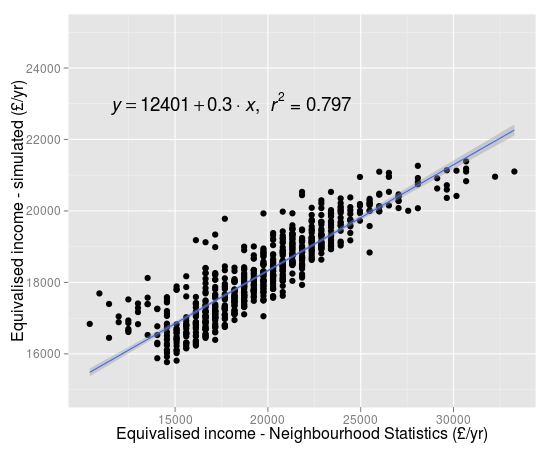
\includegraphics[width=12cm]{Income-check-morevars}
\caption[Scatter plot of simulated vs official estimated income]{Scatter plot
illustrating the correlation between mean
income simulated from the model and official estimates at the MSOA
leve.}
 \label{fig:income-test}
\end{figure}

The results show the microsimulation model could be used to predict income
(modelled income), accounting for almost 80\% of the variation in the
Neighbourhood Statistics data using an ordinary least squares (OLS) regression
model.
This is impressive, given that the aim of the model is not to simulate
income but energy costs of work travel, based on mode, distance, age/sex
and class. Of these socio-economic class is the only constraint
variable traditionally thought to be closely associated with income.
The main problem with the income estimates generated through spatial
microsimulation is the small range of estimates simulated:
the standard deviation was
\pounds1,194 and \pounds3,596 for the simulated and National Statistics data
respectively. (Note the
differences in the x and y axis scales in \cref{fig:income-test}.)
This underestimation of variance can be explained because social class,
distance and modes of transport are not sufficient to determine the true
variability in household incomes. Constraining by car ownership and tenure
variables would be likely to improve the fit.

The purpose of this fitting exercise is not so much to provide accurate income
estimates at the local level but to evaluate the
performance of the spatial microsimulation model. In terms of income, a variable
that is unconstrained in the model yet available from the survey data, the
spatial microsimulation model has worked well. The results suggest that the
values of unconstrained variables will not simply repeat the national average
for every small area, but will vary based on how their variation at the
national level is related to the constraint variables. In this case, the
assumption that the relationships between the target variable (income) and
constraint variables at the local level (in Yorkshire and the Humber) are
similar to the relationships between these variables at the national level,
receives support. How well does the model simulate other target variables such
as environmental habits, domestic energy use and levels of deprivation?
These are interesting
questions that merit further attention based on available data.

The second approach relies on Nomis, which provides cross-tabulations of census
variables, for example transport mode by class. The downside is that the data
are randomised, as stated at the bottom of each of their small-area census
tables: ``Figures have been randomly adjusted to avoid the release of
confidential data'' (this phrase appears in many of Nomis's tables.
One example can be found here:
\href{http://www.nomisweb.co.uk/livelinks/4652.xls}{http://www.nomisweb.co.uk/livelinks/4652.xls}).

In order to harness Nomis data to test the accuracy of the microsimulation
model for calculating, it was first necessary to establish how accurate Nomis
data are. How much have Nomis data been randomised, and in what way? 
This question is relatively easy to 
answer because of the census variables shared between those published 
by Nomis and by Casweb at the MSOA level. Scatter plots
suggest Nomis data are faithful to the original census results:

\begin{figure}[h]
 \centering
 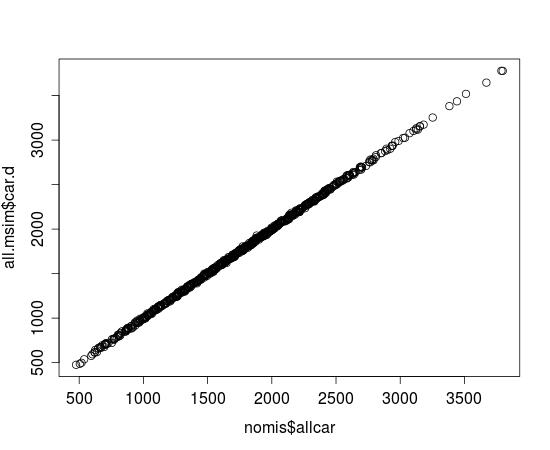
\includegraphics[width=6.6cm]{nomis-vs-cens-car}
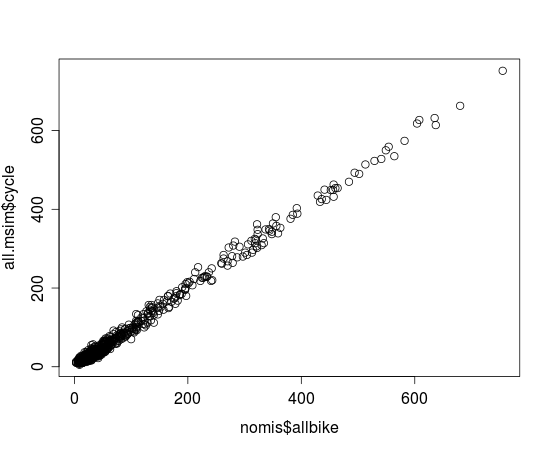
\includegraphics[width=6.6cm]{nomis-vs-cens-bike}
 % Graph-line.pdf: 516x363 pixel, 72dpi, 18.20x12.81 cm, bb=0 0 516 363
 \caption[Scatter plot of error introduced in Nomis data]{Scatter graphs
illustrating the fit between Nomis
and Casweb versions of the same census variables. The correlation (Pearson's r)
is 0.9998 and 0.9969, for the number of car drivers and number of cyclists in
each MSOA respectively.}
 \label{fig:nomis-vs-cens-car}
\end{figure}

From \cref{fig:nomis-vs-cens-car} it is interesting to note that the
correlation decreases for cyclists. This, it was inferred, could represent
an increase in the signal-to-noise ratio for variables with small values
to a fixed randomising factor.  To test this, the errors were plotted for
variables with large (car drivers) and small (cyclists) totals. The results
indicate that the noise added by randomisation is equal for each variable,
regardless of the cell count (\cref{fig:nomis-ers}).

 \begin{figure}[h]
 \centering
 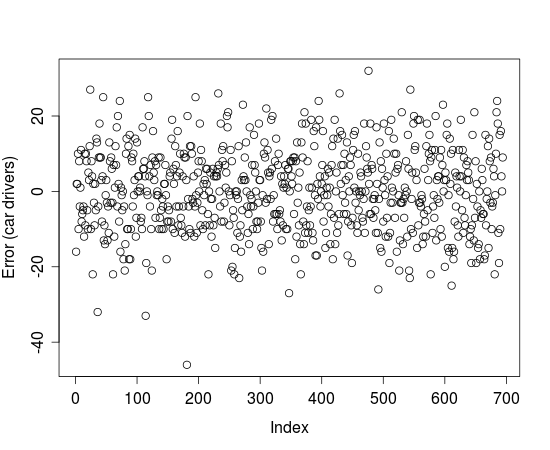
\includegraphics[width=6.6cm]{car-ers}
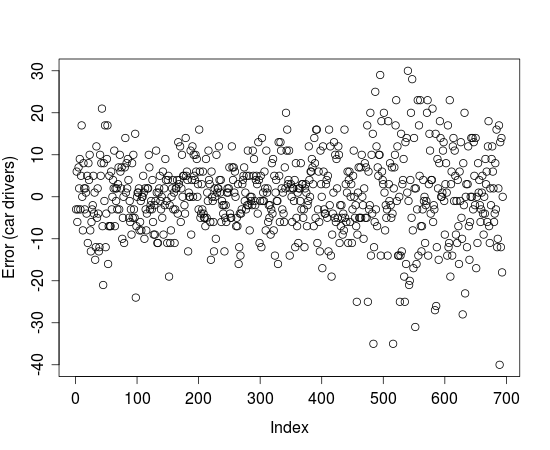
\includegraphics[width=6.6cm]{bike-ers}
 % Graph-line.pdf: 516x363 pixel, 72dpi, 18.20x12.81 cm, bb=0 0 516 363
 \caption[Errors associated with Casweb census variables]
{Errors (Casweb values -- Nomis values) associated with car driver
(right) and bicycle commuter (left) census variables.}
 \label{fig:nomis-ers}
\end{figure}

The errors seem to be similar, with a range of approximately 70 and a mean of
zero. This observation is confirmed by descriptive statistics for each set of
errors (standard deviation = 11.01, 9.47; mean = 0.15, 0.23) for car driver and
cyclist variables respectively. We can therefore conclude that the error added
by randomisation is constant for each variable and this was confirmed by plotting
the errors for additional census variables. Q-Q plots --- which compare the 
quantile values of one distribution against another, in this case those of 
the errors against those of the normal distribution --- suggest that the
distribution of error is approximately normal.

These exploratory methods provide confidence in the Nomis data, but only for
relatively large cell counts (the signal-noise ratio approaches 1:1 as the cell
count approaches 20): therefore evaluations based on Nomis data are better
suited to cross tabulated categories that have high cell counts, for example car
drivers. In our microsimulation model, both gender and mode of
transport are constrained, but not simultaneously, so the fit between the Nomis
cross-tabulation and the cross-tabulation resulting from our model provides
some indication of accuracy. The results are presented in
\cref{no-vs-sim-mcar}. Interestingly, the accuracy of this `partially
constrained' simulated target variable appears to be worse than that of the
completely unconstrained income variable (compare \cref{no-vs-sim-mcar}
and \cref{fig:income-test}). In both cases, the correlation is reasonably strong
and positive (0.47 and 0.80 respectively). However, as with the income
estimates, the \emph{distribution} of estimates arising from the model
is less dispersed than actual data: the standard deviation for the former (0.30)
is substantially less than for the latter (0.44). This illustrates the tendency
of spatial microsimulation models to underestimate the extent of spatial
variation. %%% citep{} ???

\begin{figure}
 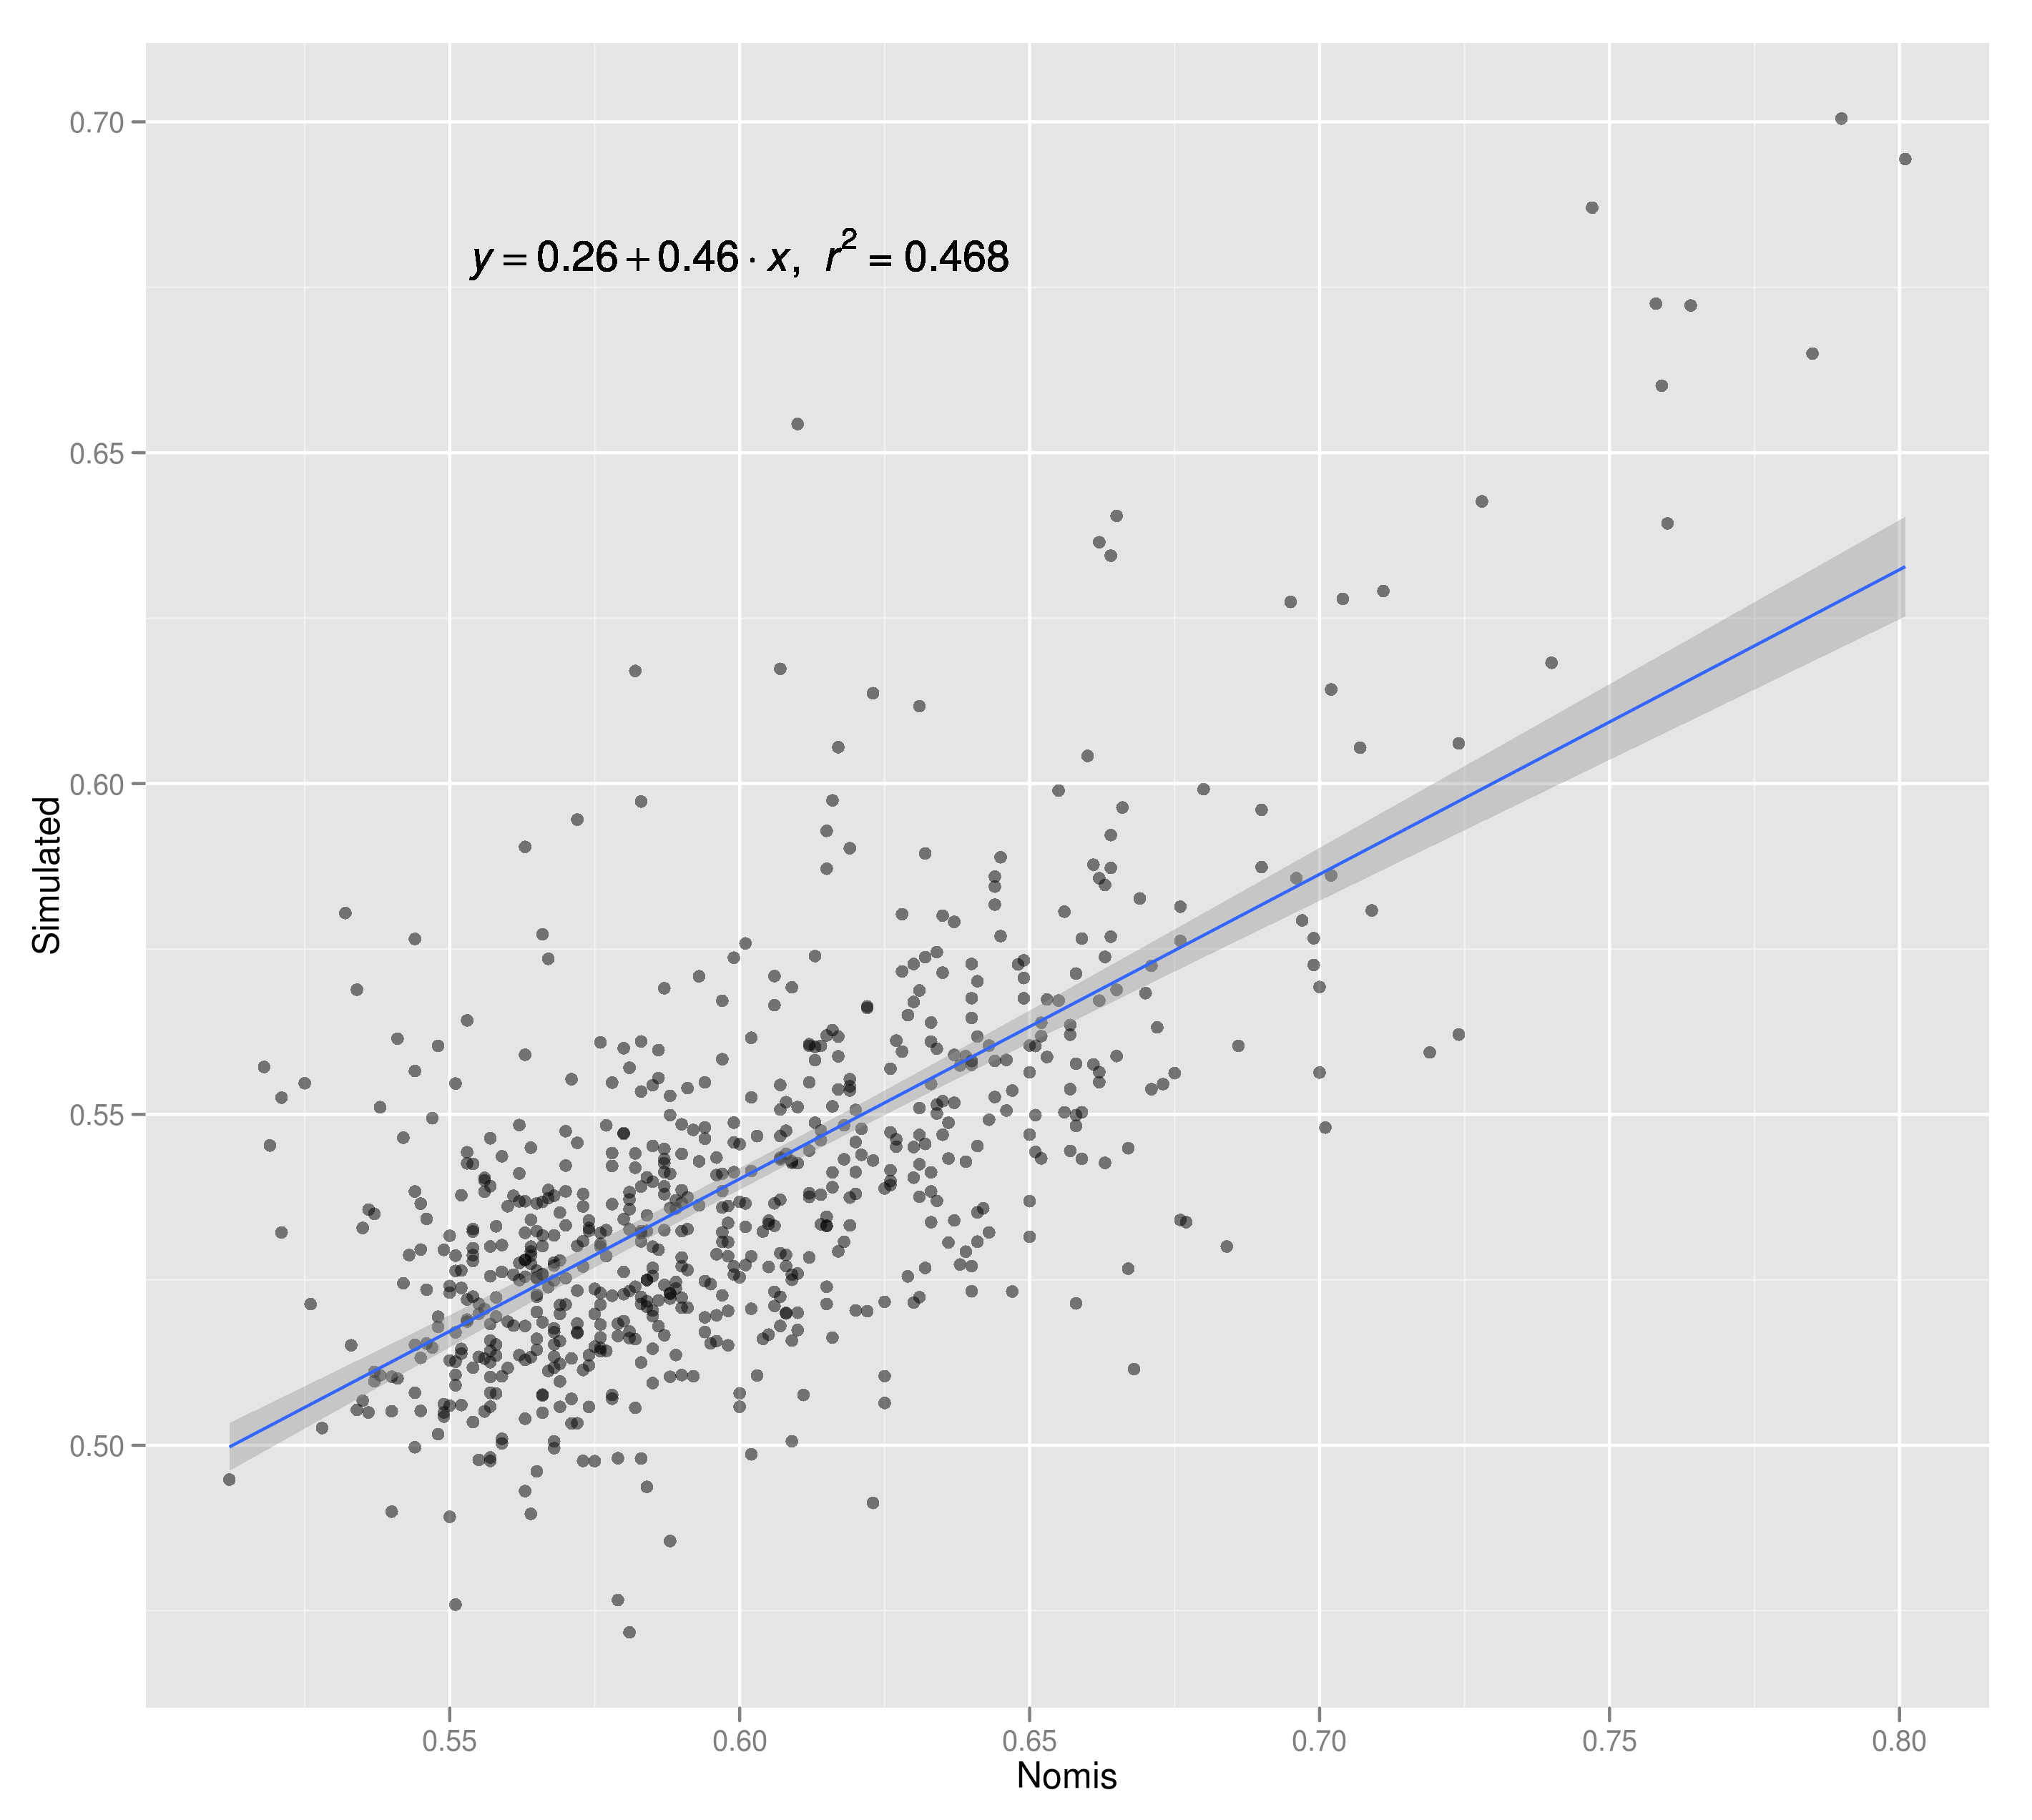
\includegraphics[width = 12 cm]{no-vs-sim-mcar}
\caption[Scatter plot of the proportion of male drivers]{Scatter plot of
the proportion of male drivers in each MSOA area in
Yorkshire and the Humber according to simulated and Nomis data.}
\label{no-vs-sim-mcar}
\end{figure}

\subsection{Additional validation methods}
The methods described above illustrate the techniques used to prevent
model errors and ensure that the results were compatible with external data
sources. But they only scratch the surface of what is possible in terms of
model validation. This section will not go into detail. Its
purpose is to draw attention to
additional methods that could be conducted as lines of future research
and discuss the merits of each. Specifically, the following additional validation
methods could (given sufficient resources) be implemented:
\begin{itemize}
 \item Primary data collection of target variables at the individual level
 in specific areas to  validate the spatial microdata locally.
 \item Comparing of the spatial microdata over entire region with a
 survey data that specifies home region of resident.
 \item Aggregating local model outputs to coarser geographical levels at which
 cross-tabulated data are available.
 \item Comparison of mode and distance data with external correlates of personal
 travel (e.g.~MOT data on distance travelled and bus usage data).
\end{itemize}

Other than the sanity check of age-sex ratios presented in \cref{fasp},
the evaluation methods considered above operate at the level of geographically
aggregated counts. However, the unique feature of spatial microsimulation is
its simulation of individuals. Evaluation techniques should therefore operate
at the individual level as well.
% The potential for evaluation of the simulated
% spatial microdata outputs is limited by the availability of official spatial
% microdata. As a result this section is short and, for the most part,
% purely theoretical.
%
% The available datasets were introduced with reference to an idealised
% `perfect' dataset on commuting \cref{fdata-ideal}. In the same way, we will
% describe methods of evaluating the microsimulation model at the individual
% level with reference to the ideal of unlimited data. This will inform the
% discussion of how best to use the individual level data that is available
% for model evaluation...
Because simulation, almost by definition, estimates something that is not
otherwise known, it is hard to find reliable individual level
data against which the estimates can be evaluated. For this reason
individual level surveys could be conducted in a specific area where
spatial microdata have been generated. To take one example, a randomised
sample of households could be taken in a single ward. Respondents would be
asked the mode of travel to work, distance and frequency of trip and
other variables. This would allow the model to be evaluated
not only in terms of the correlations that it outputs between different categories,
but also for the evaluation of the assumptions on which the energy calculations %??? where
are based.

One of the main advantages %cited where???
of spatial microsimulation over just using aggregated data is that it provides
insight into the \emph{distribution} of continuous variables within each zone,
rather than just counts of categories which are often rather coarse. T-tests and
Analysis of Variance (ANOVA) tests could then be used to check if the
mean and variance of the simulated and survey data are statistically likely
to be from the same population. However, the raw results of IPF are not
conducive to such tests at the individual level because they do not contain
whole individuals. Integerisation of the weight matrices is needed.


\section{Integerisation} \index{integerisation}
\label{s:integerisation}
An important advantage of spatial microsimulation models is their ability
to model individuals. Yet, as shown in the previous section, the IPF
procedure does not result in whole individuals, but fractions of individuals.
This is not a problem if the aim of spatial microsimulation is \emph{small area
estimation} \citep{Ballas2005b}. However, the potential to model individual
people using agent-based modelling techniques can make spatial microsimulation
much more powerful. One way to tackle this issue is by using a different
reweighting strategy to select representative individuals for each area.
An alternative is to convert the results of IPF into
integer results. \citet{Lovelace2013-trs} tackled this issue in detail and
developed a new method of integerisation. The following section is therefore
based on \citet{Lovelace2013-trs} and repeats much of the content.

The aim of IPF, as with all spatial microsimulation methods, is to  match
individual level data from one source to aggregated data from another.
IPF does this repeatedly, using one constraint variable at a time: each
brings the column and row totals of the simulated dataset closer to
those of the area in question (see \citealp{Ballas2005b} and
Fig.~\ref{fig:IPF-4c} below).

Unlike combinatorial optimisation algorithms, IPF results in non-integer
weights. As mentioned above, this is problematic for certain applications.
In their overview of methods for spatial microsimulation
\citet{Williamson1998} favoured combinatorial
optimisation approaches, precisely for this reason:
%It should be noted that only integer reweighting schemes are to be considered
``as non-integer weights lead, upon tabulation of results, to fractions of
households or individuals'' (p.\ 791). There are two options
available for dealing with this problem with IPF:
\begin{itemize}
\item Use combinatorial optimisation microsimulation methods instead
\citep{Williamson1998}. However, this can be computationally intensive
\citep{Pritchard2012}.
\item Integerise the weights: Translate the non-integer weights obtained
through IPF into discrete counts of individuals selected from the original
survey dataset \citep{Ballas2005c}.
\end{itemize}
We revisit the second option, which arguably provides the
`best of both worlds': the simplicity and computational speed of deterministic
reweighting and the benefits of using whole individuals rather than fractions.
%allows for the
%use of simple IPF models to deterministically provide the best possible fit
%between
% As with any model, spatial microsimulation models are rough approximations
% of an infinitely complex reality and, as with any model, they rely on
% assumptions about how the world works. In this case the founding assumption is
% that the relationships between the constraint variables and the target
%variables
% are the same for individuals in the survey as for individuals in the
% areas under investigation. Using the example of income, its dependence on age
%is
% assumed to remain constant in each area. If young people earn less money in
%the
% survey, an area containing a high proportion of young people will be expected
%to
% have a low income relative to an area containing a low proportion of young
% people, all other factors being equal. The technique makes the assumption
% that relationships between socio-economic variables remain constant over space
% \citep{Cullinan2011}.
% composed of scattered points whose
%characteristics vary are ubiquitous in Geography,
%or `integer reweighting', as it also called \citep{Ballas2005},
%Examples of why integerisation is useful

IPF is an established method for combining microdata
with spatially aggregated constraints to simulate  target variables whose
characteristics are not recorded at the local level. Integerisation translates
the real number weights obtained by IPF into samples from the original
microdata, a list of `cloned' individuals for each simulated area.
Integerisation may also be useful conceptually, as it allows
researchers to deal with entire individuals. The next section
reviews existing strategies for integerisation.

\subsection{Method}
\label{strategies}
Despite the importance of integer weights for dynamic spatial microsimulation,
and the continued use of IPF, there
has been little work directed towards integerisation. It has been noted that
``the
integerization and the selection tasks may introduce a bias in the synthesized
population'' \citep[10]{Muller2010}, yet little work has been done to find out
\emph{how much} error is introduced.

To test each integerisation method, IPF was used to generate an
array of weights that fit individual level survey data to
geographically aggregated census data (see Section \ref{worked-eg}). Five
methods for
integerising the results are described, three deterministic and two
probabilistic. These are: `simple rounding', its evolution into the `threshold
approach' and the `counter-weight' method and the probabilistic methods:
`proportional probabilities' and `truncate, replicate, sample'. TRS
builds on the strengths of the other methods, hence the order in which they are
presented.

The application of these methods to the same dataset and their implementation in R allows
their respective performance characteristics to be quantified and compared.
Before proceeding to describe the mechanisms by which these integerisation
methods work, it is worth taking a step back, to consider the nature and
meaning of IPF weights.

\subsubsection{Interpreting IPF weights: replication and probability}
It is important to clarify what is meant by `weights' before proceeding to
implement methods of integerisation: this understanding was central to the
development of the integerisation method presented in this section.
The weights obtained through IPF are real numbers ranging from 0 to hundreds
(the largest weight in the case study dataset is 311.8). This range
makes integerisation problematic: if the probability of selection is
proportional to the IPF weights, as is the case with the `proportional
probabilities' method,
the majority of resulting selection probabilities can be very low.
This is why the simple rounding method rounds weights up or down to the nearest
integer weight to determine how many times each individual should be
replicated (Ballas et al., 2005a). This ensures that replication weights do not differ
greatly from non-integer IPF weights. However, some of the information contained
in the weight is lost during rounding: a weight remainder of 0.501 is treated
the same as 0.999.

This raises the following question: Do the weights refer to the number of times
a particular individual should be replicated, or is it related to the
probability of being selected? The following sections
consider different approaches to addressing this question, and the
integerisation methods that result.


IPF weights do not merely represent the probability of a single case
being selected. They also (when above one) contain information about
repetition: the two types of weight are bound up in a single number. An
IPF weight of 9, for example, means that the individual should be replicated
9 times in the synthetic microdataset. A weight of 0.2, by contrast, means
that the characteristics of this individual should count for only 1/5 of their
whole value in the microsimulated dataset and that, in a representative
sampling strategy, the individual would have a probability of 0.2 of being
selected. Clearly, these are very different concepts. As such, the TRS approach
to integerisation isolates
the replication and probability components of IPF weights at the outset, and
then deals with each separately. Simple rounding, by contrast, interprets IPF
weights as inaccurate count data.


\subsubsection{Simple rounding}
The simplest approach to integerisation is to convert the non-integer
weights into an integer by rounding up if 
the decimal is 0.5 or above or down otherwise.
Rounding alone is inadequate for accurate results, however. As illustrated in
Fig.~\ref{fig:histws} below, the distribution of weights obtained by IPF is
likely to be skewed, and the majority of weights may fall below the critical 0.5
value and be excluded. As reported by \citet[25]{Ballas2005c}, this results in
inaccurate total populations. To overcome this problem
\citet{Ballas2005c} developed algorithms to `top up' the simulated
spatial microdata with
representative individuals: the `threshold' and `counter-weight' approaches.

\subsubsection{The threshold approach}
\citet{Ballas2005c} tackled the need to `top up' the simulated area
populations such that $Pop_{sim} \geq Pop_{cens}$. This is done by creating an inclusion
threshold ($IT$) set to 1 which iteratively
reduced. This samples additional individuals with
incrementally lower weights.\footnote{A 
more detailed description of the steps
taken and the R code needed to perform them iteratively can be found in the
Supplementary Information, Section 3.2.}
Below the exit value of $IT$ for each zone, no individuals can be included
(hence the clear cut-off point around 0.4 in Fig.~\ref{fig:threshweights}).
In its original form, based on rounded weights, this approach over-replicates
individuals with high decimal weights.
To overcome this problem, the truncated weights were taken as the starting
population, rather than the rounded weights. This modified approach improved the
accuracy of the integer results and is therefore the meaning of
the `threshold approach' henceforth.\footnote{An
explanation of this improvement can be illustrated by considering an individual
with a weight of 2.99. Under the original threshold approach described by
\citet{Ballas2005c}, this person would be replicated 4 times: three times after
rounding, and then a
fourth time after $IT$ drops below 0.99. With our modified approach they would
be replicated three times: twice after truncation, and again after $IT$ drops
below 0.99. The improvement in accuracy in our tests was substantial, from a TAE
(total absolute error, described below) of 96,670 to 66,762. Because both
methods are equally easy to implement, only to the superior
version of the threshold integerisation
method is used.}

The technique successfully tops up integer populations yet has
a tendency to generate too many individuals for each zone.
This oversampling is due to duplicate weights --- each unique weight was
repeated on average 3 times in our model --- and the presence of
weights that \emph{are} different, but separated by less than 0.001.
(In our test, the mean number of unique weights falling into
non-empty bins between 0.3 and 0.48 in each area --- the range of values
reached by $IT$ before  $Pop_{sim} \geq Pop_{cens}$ --- is almost two.)


\subsubsection{The counter-weight approach}
An alternative method for topping-up integer results arrived at by simple
rounding was also described by \citet{Ballas2005c}. The approach was labelled
to emphasise its reliance on both counter and a weight variables. Each
individual is first allocated a counter in ascending order of its IPF weight.
The algorithm then tops-up the integer results of simple rounding by iterating
over all individuals in the order of their count. With each iteration the new
integer weight is set as the rounded weight plus the rounded sum of its decimal
weight plus the decimal weight of the next individual, until the desired total
population is reached.\footnote{This process is described in more detail in the
Supplementary Information.} %%% Now do it!

There are two theoretical advantages of this approach: its more accurate
final populations (it does not automatically duplicate individuals with equal
weights as the threshold approach does) and the fact that
individuals with decimal weights down to 0.25 may be selected.
This latter advantage is minor, as $IT$ reached below 0.4 in many cases
(Supplementary Information, Fig.~2) --- not far off.
A band of low weights (just above 0.25)
selected by the counter-weight method can be seen in
Fig.~\ref{fig:threshweights}.

The total omission of weights below some threshold is problematic for all
deterministic algorithms tested here: they imply that someone with a weight
below this threshold, for example 0.199 in our tests, has the same sampling
probability as someone with a weight of 0.001: zero! The complete
omission of low weights fails to make use of all the information stored in
IPF weights: in fact, the individual with an
IPF weight of 0.199 is 199 times more representative of the area (in terms of
the constraint variables and the make-up of the survey dataset) than the
individual with an IPF weight of 0.001. Probabilistic approaches to
integerisation ensure that all such differences between decimal weights
are accounted for.

\begin{figure}[t]
 \centerline{ 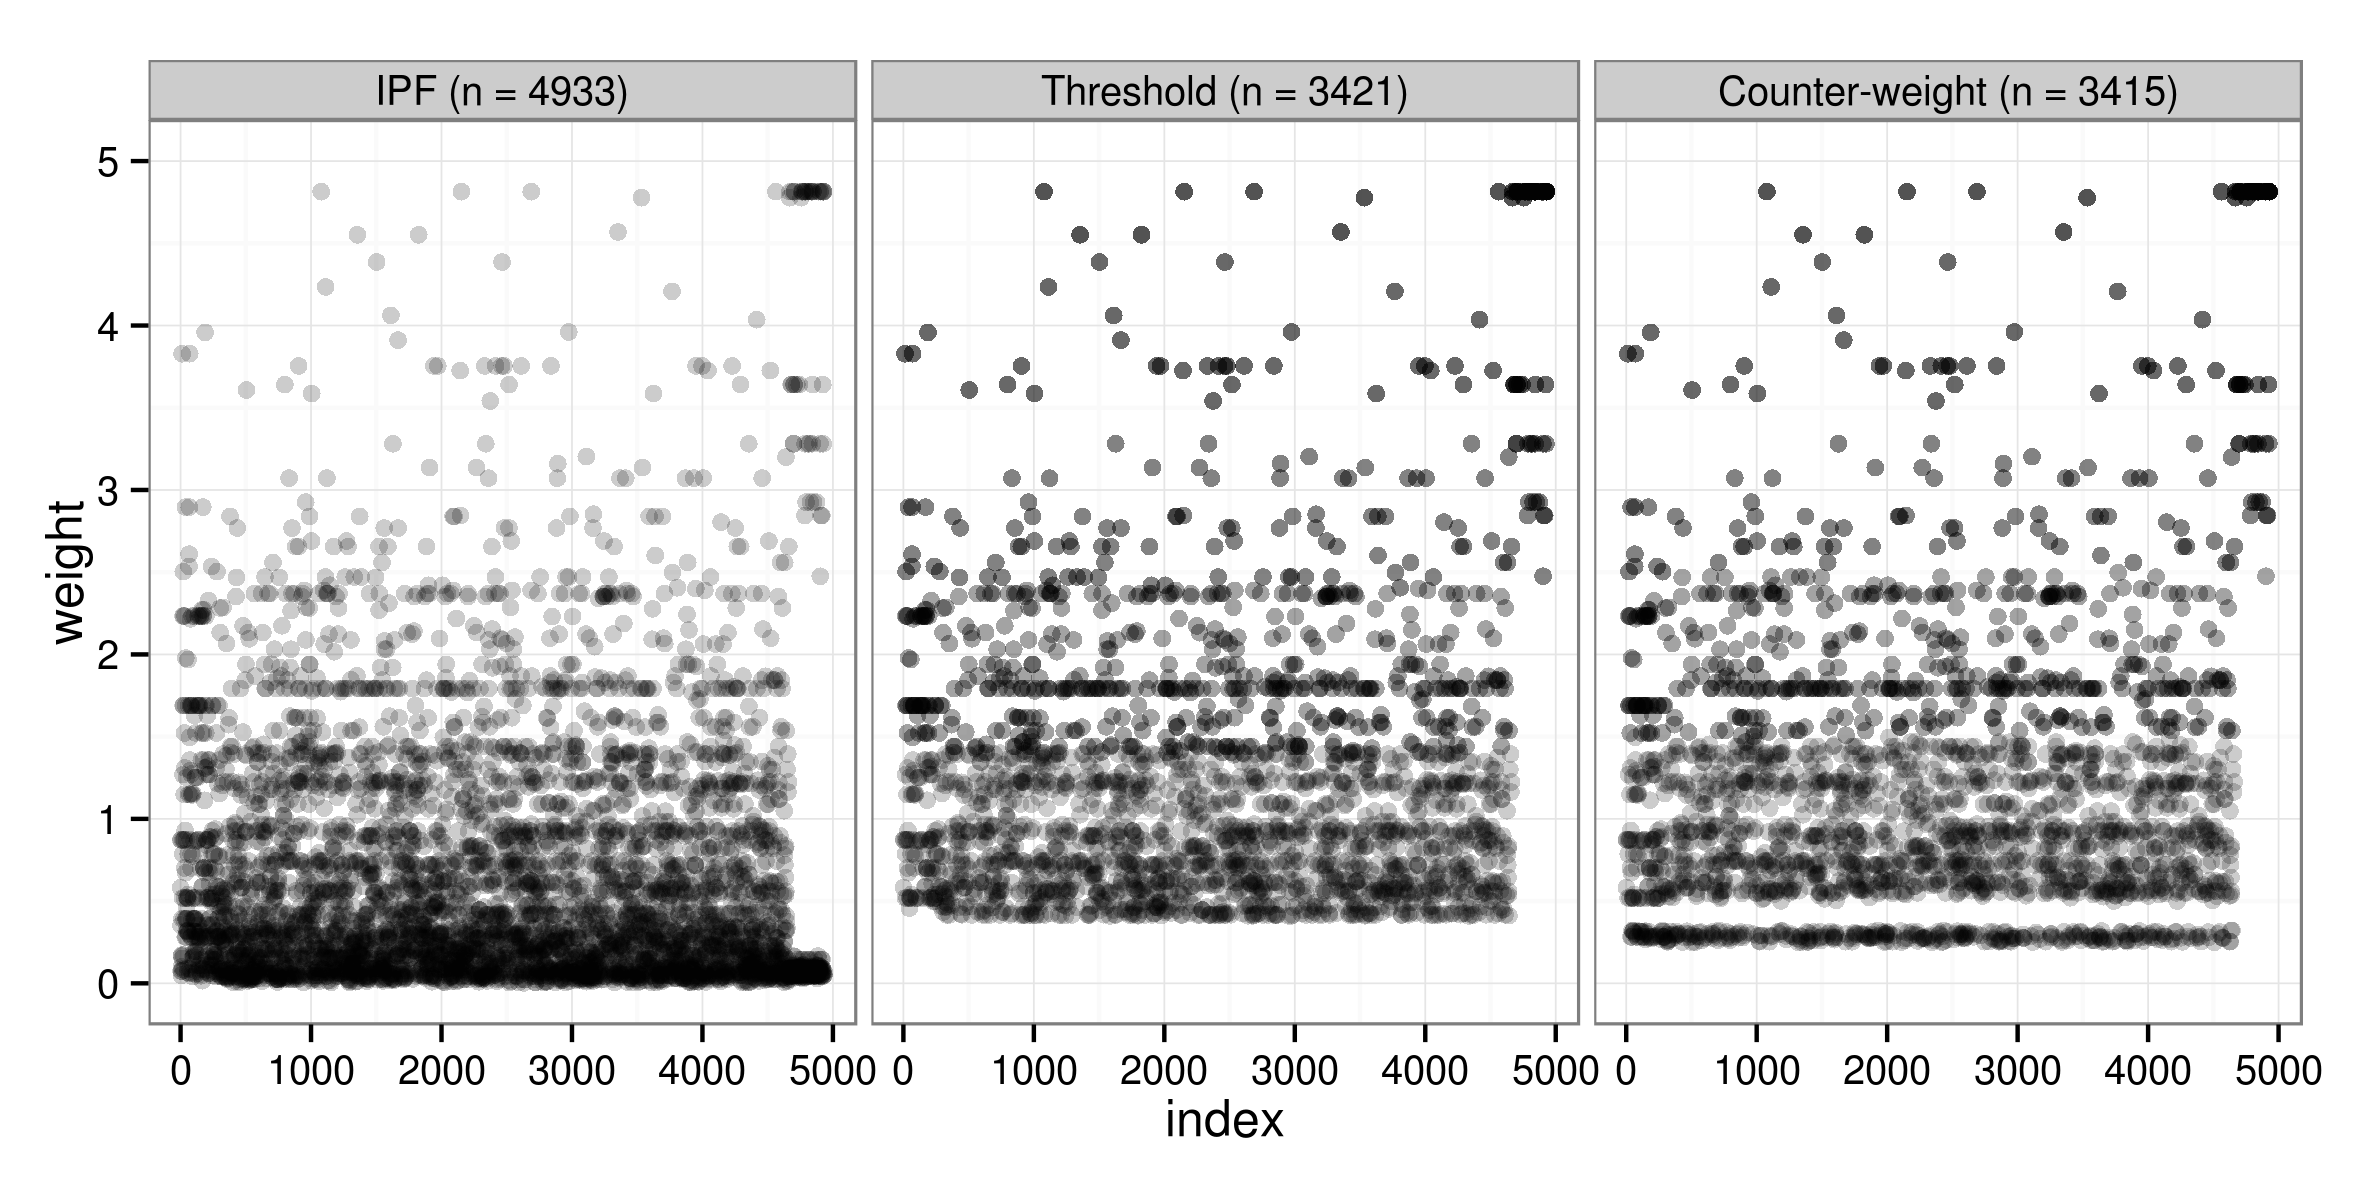
\includegraphics[width=14 cm]{IvW3}}
 % meths-scat.pdf: 792x612 pixel, 72dpi, 27.94x21.59 cm, bb=
 \caption[Overplotted scatter graph showing the distribution of IPF
weights]{Overplotted scatter graph showing the distribution of weights and
replications after IPF in the original survey (left), those selected
by inclusion thresholds for a single area (middle), and those selected
by the counter-weight method (right) for zone 71 in the
example dataset. The lightest points represent individuals who have been
replicated once, the darkest 5 times.}
 \label{fig:threshweights}
\end{figure}

% \begin{figure}[t]
%  \centerline{ 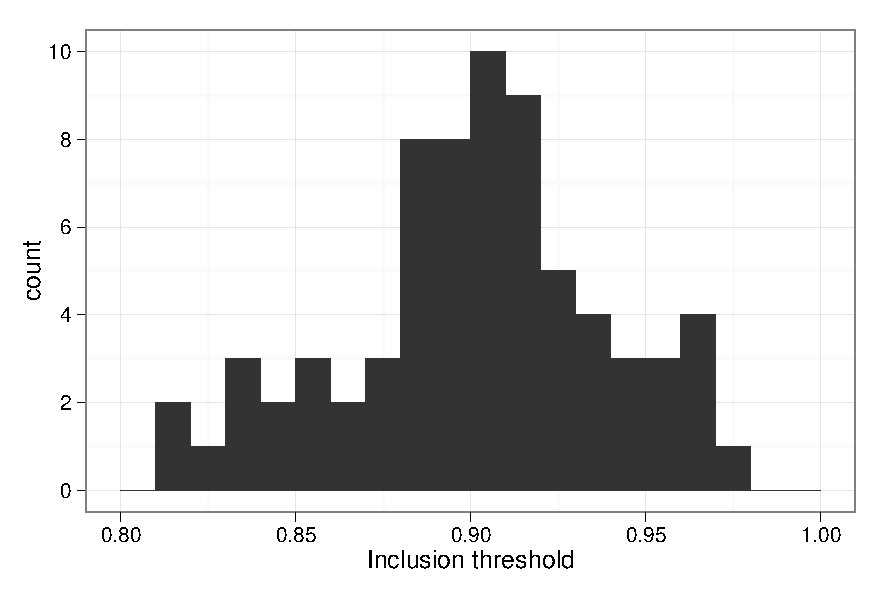
\includegraphics[width=14 cm]{Inclusion-hist2.pdf}}
%  % meths-scat.pdf: 792x612 pixel, 72dpi, 27.94x21.59 cm, bb=
%  \caption{Histogram of the inclusion thresholds ($IT$) reached in order
% to `top-up' individuals selected by simple rounding. (n = 71 zones.)}
%  \label{fig:Inclusion-hist}
% \end{figure}

\subsubsection{The proportional probabilities approach}
This approach to integerisation treats IPF weights as probabilities.
The chance of an individual being selected is proportional to the IPF
weight:
\begin{equation}
 p = \frac{w}{\sum{W}}
\end{equation}
Sampling until $Pop_{sim} = Pop_{cens}$ \emph{with replication} ensures that
individuals with high weights are likely to be repeated several times
whereas individuals with low weights are unlikely to appear.
% Due to the law of rare events, the probability that an individual with
% weight $w$ will appear  $X \in \mathbb{N}$ times in the integerised results
% follows
% the Poisson distribution:
% \begin{equation}
% p\left( X \right) = \frac{{e^{ - w } w ^X }}{{X!}}
% \end{equation}
The outcome of this strategy is correct from a theoretical perspective,
yet because all weights are treated as
probabilities, there is a non-zero
chance that an individual with a low weight
(e.g.~0.3) is replicated
more times than an individual with a higher weight (e.g.~3.3). (In this
case the probability for any given area is $\sim$ 1\%, regardless of the
population size). Ideally, this should never happen: the individual with weight
0.3 should be replicated either 0 or 1 times, the probability of the latter
being 0.3. The approach described in the next section addresses these issues.

\subsubsection{Truncate, replicate, sample}
\label{s:trs}
The problems associated with the aforementioned integerisation strategies
demonstrate the need for an alternative method.
Ideally, the method would build upon the simplicity of the
rounding method, select the correct simulated population size (as attempted by
the threshold approach and achieved by using `proportional probabilities'),
make use of all the information stored in IPF
weights \emph{and} reduce the error introduced by integerisation to a
minimum. The probabilistic approach used in `proportional probabilities'
allows multiple answers to be calculated (by using different `seeds').
This is advantageous for analysis of uncertainty introduced by the
process and allows for the selection of the best fitting result.
Consideration of these design criteria led us to
develop TRS integerisation, which interprets weights as
follows: IPF weights do
not merely represent the probability of a single case being selected. They
also (when above one) contain information about repetition: the two
types of weight are bound up in a single number. An IPF weight of 9, for
example, means that the individual should be replicated 9 times in the
synthetic microdataset. A weight of 0.2, by contrast, means that the
characteristics of this individual should count for only 1/5 of their whole
value in the microsimulated dataset and that, in a representative
sampling strategy, the individual would have a probability of 0.2 of
being selected. Clearly, these are different concepts. As such, the
TRS approach to integerisation isolates the replication and probability
components of IPF weights at the outset, and then deals with each separately.
Simple rounding, by contrast, interprets IPF weights as inaccurate count data.
The steps followed by the TRS approach are  described in detail below.

\emph{Truncate}

By removing all information to the right of the decimal point, truncation
results in integer values --- integer replication weights that
determine how many times each individual should be `cloned' and placed into the
simulated microdataset. In R, the following command is used: \begin{verbatim}
count <- trunc(w)
\end{verbatim}
% This command is identical to integer division by 1 \begin{verbatim}
% x %/% 1
% \end{verbatim},
where \verb w \ is a matrix of individual weights.  Saving these values (as
\verb count ) will later ensure  that only whole integers are counted. The
decimal remainders (\verb dr ), which vary between 0 and 1, are saved by
subtracting the integer weights from the full weights:\begin{verbatim}
dr <- w - count
\end{verbatim}
This separation of conventional and replication weights provides the
basis for the next stage: replication of the integer weights.

\emph{Replicate}

In spreadsheets, replication refers simply to copying cells of
data and pasting them elsewhere. In spatial microsimulation, the
concept is no different. The number of times a
row of data is replicated depends on the integer weight: an IPF
weight of 0.99, for example, would not be replicated at this stage
because the integer weight (obtained through truncation) is 0.

To reduce the computational requirements of this stage, it is best
to simply replicate the row number (\verb index ) associated with
each individual, rather than replicate the entire row of data. This
is illustrated in the following code example, which appears
within a loop for each area (\verb i ) to be simulated:
\begin{verbatim}
 ints[[i]] <- index[rep(1:nrow(index),count)]
\end{verbatim}

Here, the indices (of weights above 1, \verb index ) are selected
and then repeated. This is done using the function \verb rep() .
The first argument (\verb 1:nrow(index) ) simply defines
the indices to be replicated; the second (\verb count )
refers to the integer weights defined in the previous subsection.
(Note: \verb count \ in this context refers only to the
integer weights above 1 in each area).
 Once the replicated indices have been generated, they
can then be used to look up the relevant characteristics of
the individuals in question.

\begin{figure}[h]
 \centerline{ 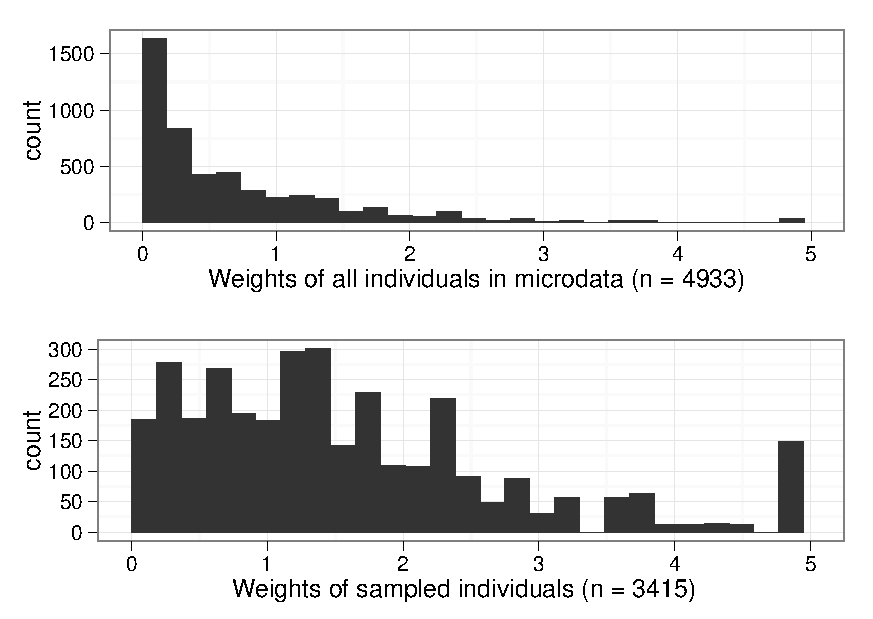
\includegraphics[width=14 cm]{hist-weights2.pdf}}
 % hist-weights.pdf: 792x612 pixel, 72dpi, 27.94x21.59 cm, bb=0 0 792 612
 \caption[Histograms of original microdata and integerised weights]{Histograms
of original microdata weights (above) and sampled microdata after TRS
integerisation (below) for a single area --- zone 71 in the case study data.}
 \label{fig:histws}
\end{figure}

\emph{Sample}

As with the rounding approach, the truncation and replication stages alone
are unable to produce microsimulated datasets of the correct size. The problem
is exacerbated by the use of truncation instead of rounding: truncation is
guaranteed to produce integer microdataset populations
that are smaller, and in some cases much smaller than the actual (census)
populations. In our case study,
the simulated microdataset populations were around half the
actual size populations defined by the census. This under-selection of
whole cases has the following advantage: when using truncation there
is no chance of over-sampling, avoiding the problem of
simulated populations being slightly too large, as can occur
with the threshold approach.

Given that the replication weights have already been included in steps 1 and 2,
only the decimal weight remainders need to be included. This can be done using
weighted random sampling without replacement. In R, the following function is
used:
\begin{verbatim}
  sample(w, size=(pops[i,1] - pops[i,2]), prob= dr[,i])
\end{verbatim}
Here, the argument \verb size \ within the \verb sample \ command is set as the
difference between the known population of each area (\verb pops[i,1] ) and
the size obtained through the replication stage alone (\verb pops[i,2] ). The
probability (\verb prob ) of an individual being sampled is determined by the
decimal remainders. \verb dr \ varies between 0 and 1, as described above.

The results for one particular area are presented in Fig.~\ref{fig:histws}.
The distribution of selected individuals has shifted to the right, as
the replication stage has replicated individuals as a function of their
truncated
weight. Individuals with low weights (below one) still constitute a large
portion of those selected, yet these individuals are replicated fewer times.
After TRS integerisation individuals with high decimal weights are relatively
common. Before integerisation, individuals with IPF weights between 0 and 0.3
dominated. An individual-by-individual visualisation of the Monte Carlo
sampling strategy is provided in Fig.~\ref{fig:index-weight-TRS}. Comparing
this with the same plot for the probabilistic methods
(Fig.~\ref{fig:threshweights}), the most noticeable difference is that the TRS
and proportional probabilities approaches
include individuals with very low weights. Another important difference is
average point
density, as illustrated by the transparency of the dots: in
Fig.~\ref{fig:threshweights}, there are shifts near the decimal
weight threshold ($\sim$ 0.4 in this area) on the y-axis.
In Fig.~\ref{fig:index-weight-TRS}, by contrast, the transition is
smoother: average darkness of single dots (the number of replications)
gradually increases from 0 to 5 in both probabilistic methods.

\begin{figure}[h]
 \centerline{
 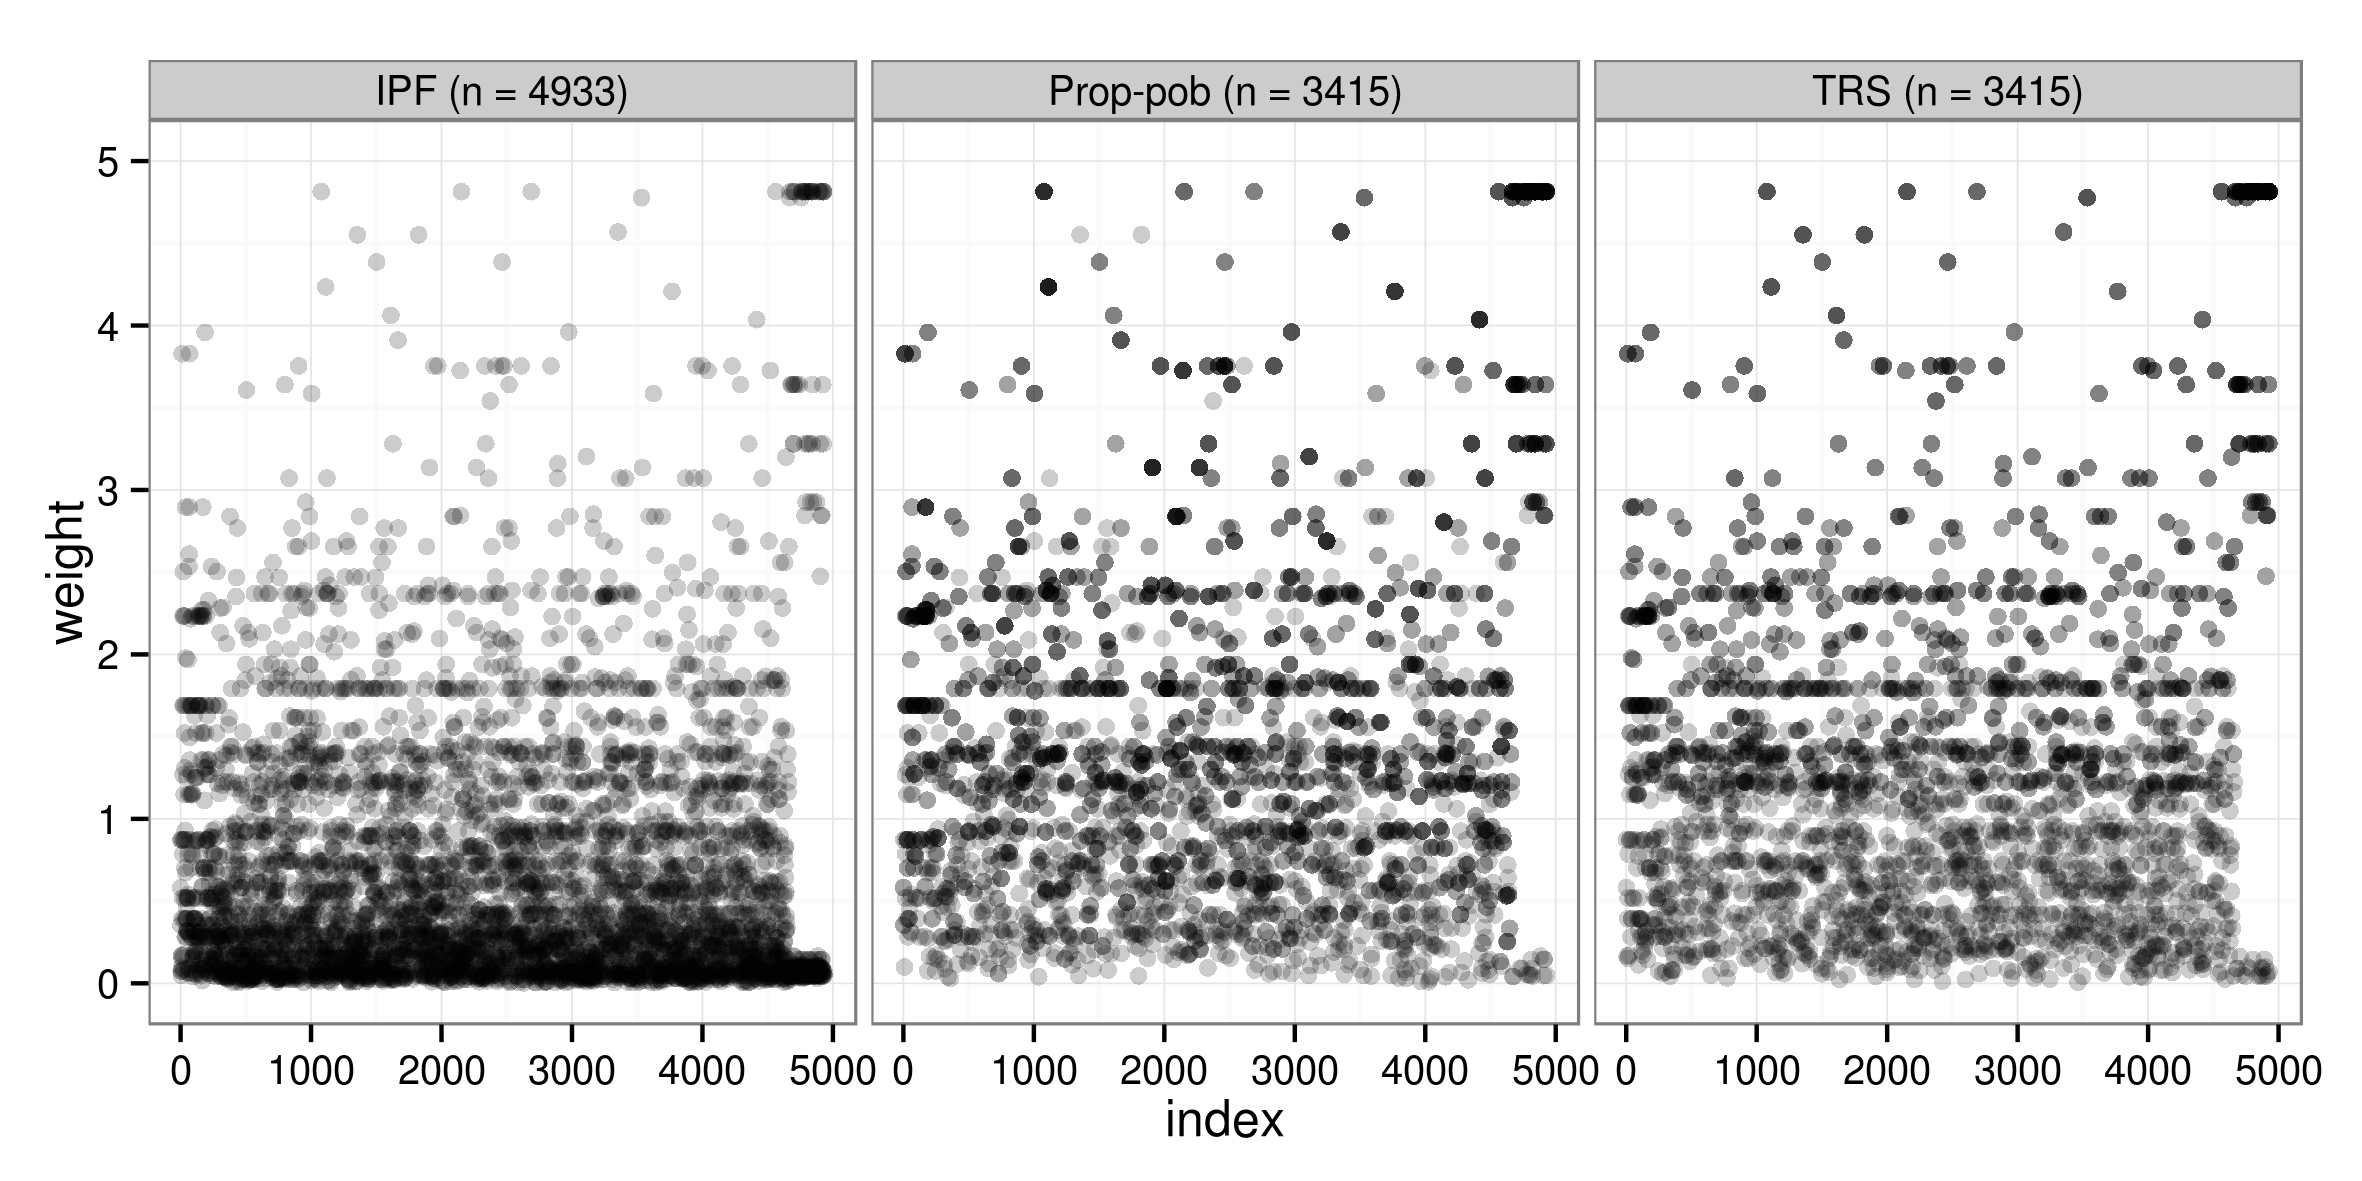
\includegraphics[width=12 cm]{IvW2}}
 % hist-weights.pdf: 792x612 pixel, 72dpi, 27.94x21.59 cm, bb=0 0 792 612
 \caption[Overplotted scatter graphs of index against weight]{Overplotted
scatter graphs of index against weight  for the original IPF weights (left) and
after proportional  probabilities (middle) and TRS (right) integerisation for
zone 71. Compare with Fig.~\ref{fig:threshweights}.}
 \label{fig:index-weight-TRS}
\end{figure}

Fig.~\ref{fig:index-TRS} illustrates the mechanism by which the TRS sampling
strategy works to select individuals. In the first stage (up to x = 1,717,
in this case) there is a linear
relationship between the indices of survey and sampled individuals, as the
model iteratively moves through the individuals, replicating those with
truncated weights greater than 0. This
(deterministic) replication stage selects roughly half of the required
population
in our example dataset (this proportion varies from zone to zone).
The next stage is probabilistic sampling
(x = 1,718 onwards in Fig.~\ref{fig:index-TRS}): individuals are selected from
the entire microdataset with selection probabilities equal to weight remainders.


\begin{figure}[h]
 \centerline{
 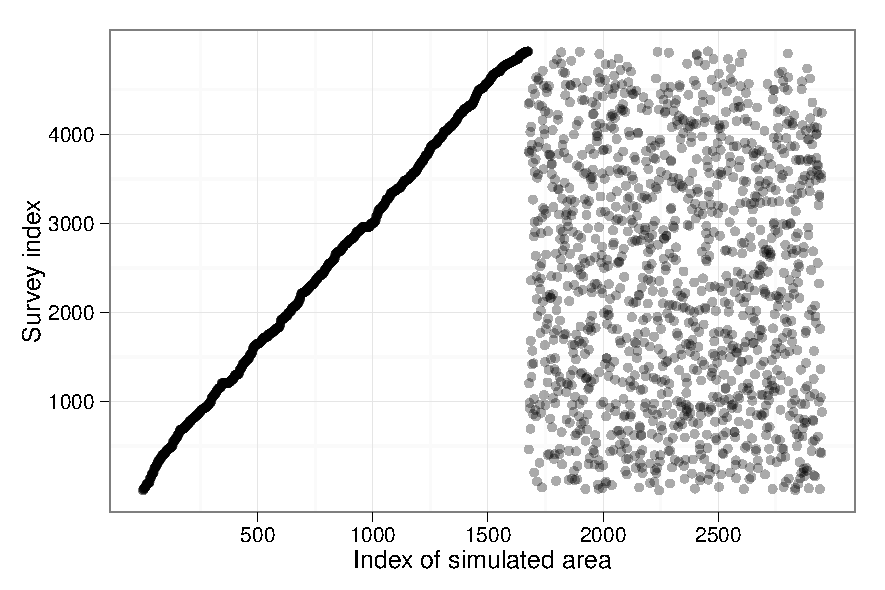
\includegraphics[width=12 cm]{indexes.pdf}}
 % hist-weights.pdf: 792x612 pixel, 72dpi, 27.94x21.59 cm, bb=0 0 792 612
 \caption[Scatter graph of the index values of individuals]{Scatter graph of the
index values of individuals in the original sample and their indices following
TRS Integerisation for a single area. }
 \label{fig:index-TRS}
\end{figure}

\subsubsection{The test scenario: input data and IPF}
\label{worked-eg}
% In order to test integerisation techniques, they were tested on a real world
% example. This section serves two functions: to illustrate the utility of
% integerisation techniques when modelling continuous variables using spatial
% microsimulation, and to describe how the integerisation
% techniques were tested.
The theory and methods presented above demonstrate how five integerisation
methods work in abstract terms. But to compare them quantitatively a test
scenario is needed. This example consists of a spatial microsimulation model
that uses IPF to model the commuting and socio-demographic characteristics
of economically active individuals in
Sheffield. According to the 2001 Census, Sheffield has a working
population of just over 230,000. The characteristics of these
individuals were simulated by reweighting a synthetic microdataset based on
aggregate constraint variables provided at the medium super output area (MSOA)
level. The synthetic microdataset was created by `scrambling' a subset of the
Understanding Society dataset (USd).\footnote{See
http://www.understandingsociety.org.uk/. To scramble this data, the continuous
variables (see Table \ref{t:data}) had an integer random number (between 10 and
-10) added to them; categorical variables were mixed up, and all other
information was removed.} MSOAs
contain on average
just over 7,000 people each, of whom 44\% are economically active
in the study area; for the less sensitive aggregate constraints, real data were
used. These variables are summarised in Table \ref{t:data}.

\begin{table}[htbp]
\caption{Summary data for the spatial microsimulation model}
\begin{center}
\begin{tabular}{lrlll}
\toprule
 & \multicolumn{ 2}{c}{\textbf{Aggregate data}} & \multicolumn{
2}{c}{\textbf{Survey data}} \\
 & \multicolumn{ 2}{c}{71 zones, average pop.: 3077.5} & \multicolumn{
2}{c}{4933 observations} \\ \midrule
Variable & \multicolumn{1}{l}{N. categories} & Most populous  & Mean  &
Most populous \\ \hline
Age / sex  & 12 & Male, 35 to 54 yrs & \multicolumn{1}{r}{40.1} & - \\
Mode  & 11 & Car driver & - & Car driver \\
Distance  & 8 & 2 to 5 km & \multicolumn{1}{r}{11.6} & - \\
NS-SEC  & 9 & Lower managerial & - & Lower managerial \\ \bottomrule
\end{tabular}\end{center}
\label{t:data}
\end{table}

The data contains both continuous (age, distance) and categorical (mode,
NS-SEC) variables. In practice, all variables are converted into categorical
variables for the purposes of IPF, however. To do this statistical
bins are used.
Table \ref{t:data} illustrates similarities between aggregate
and survey data overall (car drivers being the most popular mode of travel to
work in both categories, for example). Large differences exist between
individual zones and survey data, however: it is the role of iterative
proportional fitting to apply weights to minimize these differences.

IPF was used to assign 71 weights to
each of the 4,933 individuals, one weight for each zone. The fit
between census and weighted microdata can be seen
improving after constraining by each of the 40 variables
(Fig.~\ref{fig:IPF-4c}).
The process is repeated until an adequate level
of convergence is attained (see Fig.~\ref{fig:ipf-scat}).\footnote{What
constitutes an `adequate' level of fit has not been well defined in the
literature, as mentioned in the next section. In this example, 20
iterations were used.}
\begin{figure}[h]
 \centerline{
 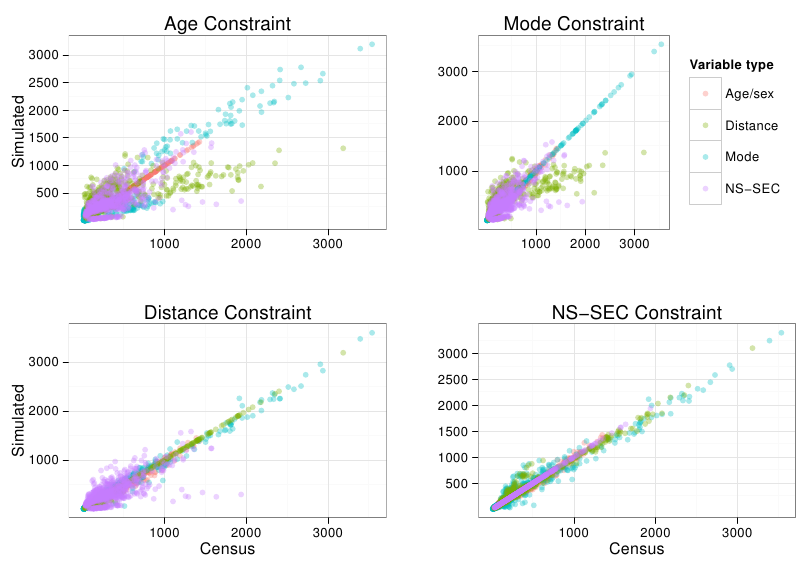
\includegraphics[width=14 cm]{IPF-4c2}}
 % hist-weights.pdf: 792x612 pixel, 72dpi, 27.94x21.59 cm, bb=0 0 792 612
 \caption[Visualisation of IPF method]{Visualisation of IPF method. The graphs
show the iterative
improvements in fit after age, mode, distance and finally NS-SEC constraints
were applied (see Table \ref{t:data}). See footnote 4 for resources on how IPF
works.}
 \label{fig:IPF-4c}
\end{figure}
The weights were set to an initial value of
one.\footnote{An initial value must be selected for IPF to create new weights
which better match the small area constraints.
It was set to one as this tends to be the average weight value in social surveys
(the mean Understanding Society dataset interview plus proxy individual
cross-sectional weight is 0.986).}
The weights were then iteratively
altered to match the aggregate (MSOA) level statistics.

\begin{figure}[h]
 \centerline{
 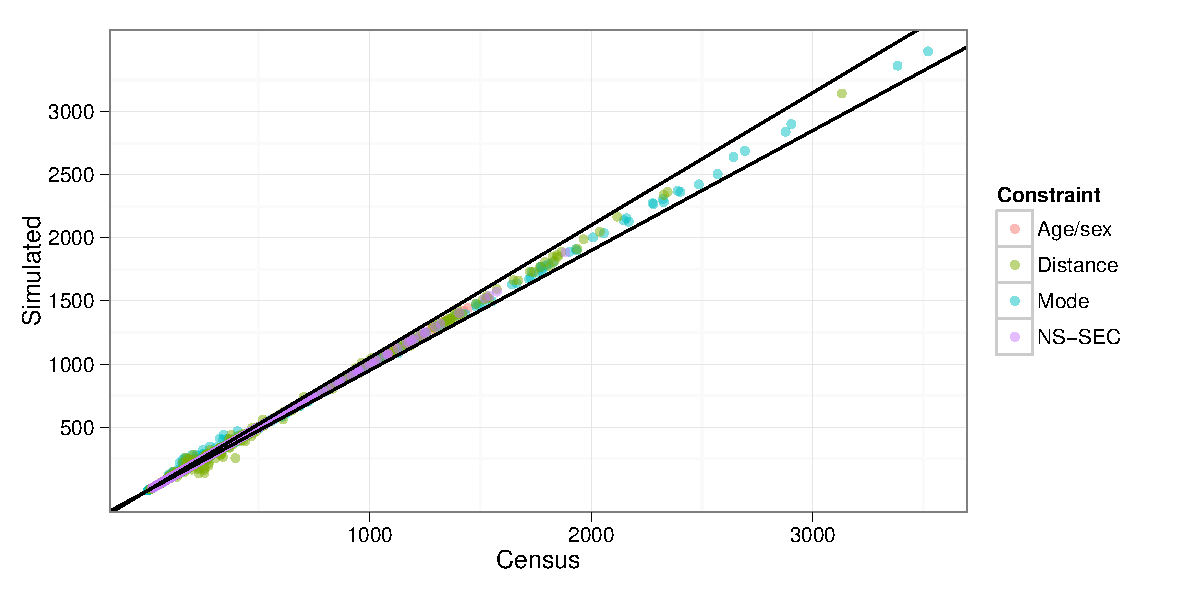
\includegraphics[width=13 cm]{ipf-scat2}}
 % hist-weights.pdf: 792x612 pixel, 72dpi, 27.94x21.59 cm, bb=0 0 792 612
 \caption[Scatter graph illustrating the fit between census and simulated
aggregates]{Scatter graph illustrating the fit between census and simulated
aggregates after 20 IPF iterations (compare with Fig.~\ref{fig:IPF-4c}).}
 \label{fig:ipf-scat}
\end{figure}

Four constraint variables link the aggregated census data to the survey,
containing a total of 40 categories. To illustrate how IPF works, it is useful
to inspect the fit between simulated and census aggregates before and after
performing IPF for each constraint variable. Fig.~\ref{fig:IPF-4c}
illustrates this process for each constraint. By contrast to existing
approaches to visualising IPF (see \citealp{Ballas2005b}), Fig.
\ref{fig:IPF-4c} plots the results for all variables, one
constraint at a time. This approach can highlight which constraint variables
are particularly problematic. After 20
iterations (Fig.~\ref{fig:ipf-scat}), one can see that distance and mode
constraints are most problematic. This may be because both variables depend
largely on geographical location, so are not captured well by UK-wide
aggregates.

Fig.~\ref{fig:IPF-4c} also illustrates how IPF works: after reweighting for
a particular constraint, the weights are forced to take values such that the
aggregate statistics of the simulated microdataset match perfectly with the
census aggregates, for all variables within the constraint in question.
Aggregate values for the mode variables, for example, fit the census results
perfectly after constraining by mode (top right panel in Fig.
\ref{fig:IPF-4c}). Reweighting by the next constraint disrupts the fit
imposed by the previous constraint --- note the increase scatter of the (blue)
mode variables after weights are constrained by distance (bottom left).

However, the disrupted fit is better than the original. This leads to
a convergence of the weights such that the fit between simulated and known
variables is optimised:
% The fit after each complete iteration can be formally measured in
% absolute and relative terms. The latter case is illustrated in Fig.~\ref{}
Fig.~\ref{fig:IPF-4c} shows that accuracy increases after weights are
constrained by each successive linking variable.
% % %\ref{fig:ints-errors},
% % %which shows how accuracy (measured as the proportion of simulated results
% % %falling beyond 5\% above or below the census value, as illustrated in
% % \ref{fig:4hists}, which shows continual improvement in model fit: the
% % distribution of residuals tend to 0 with each successive iteration.
% %
% % The results also show, however, that
% % some variables create more error than other --- the results of reweighting
% % the constraint ``mode'' are always worse than obtained by reweighting by the
% % other variables. This is significant because it means that the final results
% of
% % IPF models may depend more on the order of the constraint variables than on
% the
% % number of iterations.
%
% %  \begin{figure}[t]
% %  \centerline{
% %  \includegraphics[width=14 cm]{its-errors.pdf}}
% %  % hist-weights.pdf: 792x612 pixel, 72dpi, 27.94x21.59 cm, bb=0 0 792 612
% %  \caption{Proportion of results that fall beyond 5\% of the census values
% after
% % reweighting by each constraint variable over 10 complete iterations.}
% %  \label{fig:ints-errors}
% % \end{figure}

\subsection{Results}
\label{results}
This section compares the five previously describe approaches to
integerisation --- rounding, inclusion threshold, counter-weight, proportional
probabilities  and TRS methods. The results are based on the 20$^{th}$
iteration of the IPF model described above. The following metrics of
performance were assessed:
\begin{itemize}
 \item speed of calculation
\item accuracy of results
\begin{itemize}
 \item sample size
%: does the integer microsimulation sample size match the actual population?
\item Total Absolute Error (TAE) of simulated areas
\item anomalies (aggregate cell values out by more than 5\%)
\item correlation between constraint variables in the census and
microsimulated data.
\end{itemize}
\end{itemize}

Of these performance indicators accuracy is the most problematic.
Options for measuring goodness-of-fit have proliferated in the last two decades,
yet there is no consensus about which is most appropriate \citep{Voas2001}.
The approach taken here, therefore, is to use a range of measures, the most
important of which are summarised in Table \ref{acc-results} and Fig.
\ref{fig:3scat}.

\begin{figure}[h*]
 \centerline{
 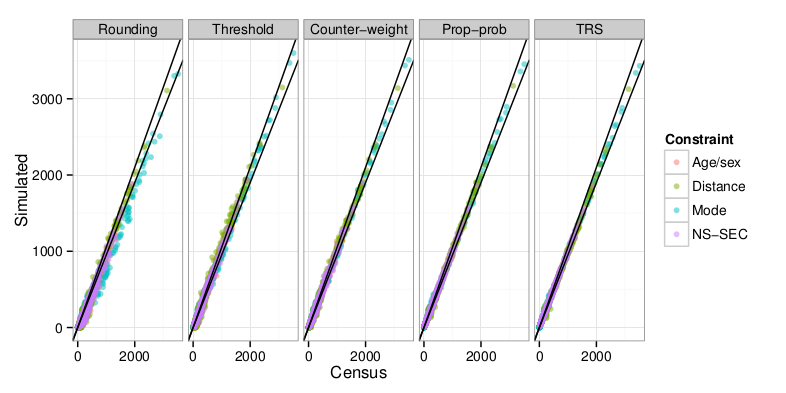
\includegraphics[width=13.5 cm]{ints-5scat-ab}}
 % hist-weights.pdf: 792x612 pixel, 72dpi, 27.94x21.59 cm, bb=0 0 792 612
 \caption[Scatterplots of actual (census) and simulated population
totals]{Scatterplots of actual (census) and simulated population totals for four
integerisation techniques. The black lines represent 5\% error in either
direction. }
 \label{fig:3scat}
\end{figure}

\subsubsection{Speed of calculation}
%With modern desktop computers, computational requirements is less frequently
The time taken for the integerisation of IPF weights was measured on an Intel
Core i5 660 (3.33 GHz) machine with 4 Gb of RAM running Linux 3.0.
The simple rounding method of integerisation was unsurprisingly the fastest, at
4 seconds. % Add c-w time
In second and third place respectively were the proportional probabilities
and TRS approaches, which took a couple of seconds longer for a single
integerisation run for all areas.
Slowest were the inclusion threshold and counter-weight techniques, which took
three times longer than simple rounding. To ensure representative results for
the probabilistic approaches, both were run 20 times and the result with the
best fit was selected. These imputation loops took just under a minute.

The computational intensity of integerisation may
be problematic when processing weights for very large
datasets, or using older computers. However, the results must be placed in
the context of the computational requirements of the IPF process itself. For the
example described in Section \ref{worked-eg}, IPF took approximately
30 seconds per iteration and 5 minutes for the full 20 iterations.

\subsubsection{Accuracy}
In order to compare the fit between simulated microdata and the zonally
aggregated linking variables that constrain them, the former must first be
aggregated by zone. This aggregation stage allows the fit between linking
variables to be compared directly (see Fig.~\ref{fig:3scat}). More
formally, this aggregation allows goodness of fit to be calculated using a range
of metrics \citep{Williamson1998}. We compared the accuracy of integerisation
techniques using 5 metrics:
\begin{itemize}
\item Pearson's product-moment correlation coefficient ($r$)
\item total and standardised absolute error (TAE and SAE),
\item proportion of simulated values falling beyond 5\% of the actual values,
% This is the standard measure
% of correlation and requires no further explanation here \citep{Rodgers1988}.
\item the proportion of Z-scores significant at the 5\% level
\item size of the sampled populations
\end{itemize}

The simplest way to evaluate the fit between simulated and census results
was to use Pearson's $r$, an established measure of association
\citep{Rodgers1988}.
The $r$ values for all constraints were 0.9911, 0.9960, 0.9978,
0.9989 and 0.9992 for rounding, threshold, counter-weight, proportional
probabilities and TRS
methods respectively. IPF alone had an $r$ value of 0.9996. These correlations
establish an order of fit that can be compared to other metrics.

TAE and SAE are crude yet effective measures of overall
model fit \citep{Voas2001}. TAE has the additional advantage of
being easily understood:
\begin{equation}
 TAE = \sum\limits_{ij}|U_{ij} - T_{ij}|
 \label{etae}
\end{equation}
where U and T are the observed and simulated values for each linking variable
($j$) and each area ($i$).
% Change 34 (symbol: % Change): converted TEA to TAE
SAE is the TAE divided by the total
population of the study area. TAE is sensitive to the number of people
within the model, while SAE is not. The latter is seen by \citet{Voas2001} as
``marginally preferable'' to the former: it allows cross-comparisons between
models of different total populations \citep{Kongmuang2006-thesis}.

\begin{table}[]
\caption{Accuracy results for integerisation techniques.*}
\small{
\begin{center}
\begin{tabular}{llrrrr}
\toprule
Method & Variables & \multicolumn{1}{l}{TAE} & \multicolumn{1}{l}{SAE (\%)} &
\multicolumn{1}{l}{E $>$ 5\% (\%)} & \multicolumn{1}{l}{$Z{m}^{2}$ (\%)} \\
\midrule
IPF & Age/sex & 9 & 0.0 & 0.0 & 0.0 \\
 & Distance & 4874 & 2.3 & 13.7 & 4.9 \\
 & Mode & 4201 & 2.0 & 6.4 & 4.2 \\
 & NS-SEC & 0 & 0.0 & 0.0 & 0.0 \\
\textbf{} & \textbf{All} & \textbf{9084} & \textbf{3.1} & \textbf{4.5} &
\textbf{2.1} \\
\midrule
Round- & Age/sex & 26812 & 12.5 & 81.5 & 39.8 \\
 ing& Distance & 31981 & 14.9 & 80.1 & 65.1 \\
 & Mode & 30558 & 14.2 & 81.4 & 48.9 \\
 & NS-SEC & 27493 & 12.8 & 76.5 & 57.1 \\
 & \textbf{All} & \textbf{116844} & \textbf{13.6} & \textbf{80.1} &
\textbf{51.3} \\
\midrule
Thresh- & Age/sex &  11076 & 5.1 & 49.2 & 8.1 \\
 old& Distance & 27146 & 12.6 & 82.4 & 57.7 \\
 & Mode & 14770 & 6.9 & 68.6 & 33.9 \\
 & NS-SEC & 13770 & 6.4 & 55.2 & 24.1 \\
 & \textbf{All} &  \textbf{66762} & \textbf{7.8} & \textbf{62.5} & \textbf{28.7}
\\
\midrule
Counter- & Age/sex & 10242 & 4.8 & 47.7 & 6.6 \\
weight& Distance &  17103 & 8.0 & 70.2 & 39.3 \\
 & Mode &  10072 & 4.7 & 60.4 & 21.6 \\
 & NS-SEC & 11798 & 5.5 & 49.6 & 17.1 \\
 & \textbf{All} & \textbf{49215} & \textbf{5.7} & \textbf{56.1} & \textbf{19.6}
\\
\midrule

Propor- & Age/sex & 9112 & 4.2 & 48.0 & 3.1 \\
tional & Distance & 8740 & 4.1 & 47.4 & 10.4 \\
proba- & Mode & 8664 & 4.0 & 60.8 & 9.0 \\
bilities & NS-SEC & 7778 & 3.6 & 37.6 & 3.3 \\
 & \textbf{All} & \textbf{34294} & \textbf{4.0} & \textbf{49.0} & \textbf{6.2}
\\
\midrule
TRS &Age/sex & 5424 & 2.5 & 27.9 & 0.4 \\
 & Distance & 10167 & 4.7 & 48.8 & 16.4 \\
 & Mode & 7584 & 3.5 & 56.1 & 6.7 \\
 & NS-SEC & 5687 & 2.6 & 24.9 & 1.1 \\
 & \textbf{Total} & \textbf{28862} & \textbf{3.4} & \textbf{39.2} & \textbf{5.5}
\\
\bottomrule
\end{tabular}
\end{center}
}
\label{acc-results}
\begin{tablenotes}
      \footnotesize
      \item * The probabilistic
results represent the best fit (in terms of TAE) of 20 integerisation runs
with the pseudo-random number seed set to 1000 for replicability --- see
Supplementary Information.
    \end{tablenotes}
\end{table}

The proportion of values which fall beyond 5\% of the actual values is a simple
metric of the quality of the fit. It implies that getting a perfect fit is not
the aim, and penalises fits that have a large number of outliers. The precise
definition of 'outlier' is somewhat arbitrary (one could just as well use 1\%).

The final metric presented in Table \ref{acc-results}
is based on the Z-statistic, a standardised measure of
deviance from expected values, calculated for each cell of data. We use $Zm$, a
modified version of the Z-statistic which is a robust measure of fit for each
cell value \citet{Williamson1998}. The measure of
fit is appropriate here as it takes into account absolute, rather than just
relative, differences between simulated and observed cell count:
\begin{equation}
 Zm_{ij} = (r_{ij} - p_{ij}) \Bigg/ \left(\frac{p_{ij}(1 -
p_{ij}))}{\sum\limits_{ij}U_{ij}}\right)^{1/2}
\end{equation}

where

\begin{center}
\begin{math}
  p_{ij} = \frac{U_{ij}}{\sum\limits_{ij}U_{ij}} \qquad and \qquad r_{ij} =
\frac{T_{ij}}{\sum\limits_{ij}U_{ij}}
\end{math}
\end{center}

To use the modified Z-statistic as a measure of overall model fit, one simply
sums the squares of $zm$ to calculate $Z{m}^{2}$. This measure can handle
observed cell counts below 5, which chi-squared tests cannot \citep{Voas2001}.

The results presented in Table \ref{acc-results} confirm that \emph{all}
integerisation methods introduce
some error. It is reassuring that the comparative accuracy is the same across
all metrics. Total absolute error (TAE), the simplest goodness-of-fit
metric, indicates that discrepancies between simulated and census data increase
by a factor of 3.2 after TRS integerisation, compared with raw
(fractional) IPF weights.\footnote{In the case of a sufficiently diverse input
survey dataset, IPF would be able to find the perfect solution: TAE would be 0
and the ratio of error would not be
applicable.}
Still, this is a
major improvement on the simple rounding, threshold and counter-weight
approaches to integerisation presented by \citet{Ballas2005c}: these increased
TAE by a factor of 13, 7 and 5 respectively.
The improvement in fit relative to the proportional probabilities method
is more modest. The proportional probabilities method increased TAE by a factor
of 3.8, 23\% more absolute error than TRS.

The differences between the simulated and actual populations ($Pop_{sim} -
Pop_{cens}$) were also calculated for
each area. The resulting differences are summarised in Table 5, which
illustrates that the counter-weight and two probabilistic methods resulted
in the correct population totals for every area. Simple rounding and threshold
integerisation methods greatly underestimate and slightly overestimate the
actual populations, respectively.

\begin{table}[h*]
\begin{center}
\caption{Differences between census and simulated populations.}
\vspace{0.25 cm}
\begin{tabular}{lrrr}
\toprule
Metric & \multicolumn{1}{l}{Rounding} & \multicolumn{1}{l}{Threshold} &
\multicolumn{1}{l}{Others (CW, PP, TRS)} \\ \midrule
Mean & -372 & 8 & 0  \\
Standard deviation & 88 & 11 & 0 \\
Max & -133 & 54 & 0 \\
Min & -536 & 0 & 0 \\
Oversample (\%) & -13 & 0.3 & 0 \\
\bottomrule
\end{tabular}
\end{center}
\label{t:pops}
\end{table}




\subsection{Discussion and conclusions}
\label{discuss}
The results show that TRS integerisation outperforms the other methods of
integerisation tested in this section.
At the aggregate level, accuracy
improves in the following order: simple rounding,
inclusion threshold, counter-weight, proportional probabilities and, most
accurately, TRS. This order of preference remains unchanged, regardless of which
(from a selection of 5) measure of goodness-of-fit is used. These results
concur with a finding derived from theory --- that ``deterministic rounding of
the counts is not a satisfactory integerization''
\citep[p.~689]{Pritchard2012}.
Proportional probability and TRS methods clearly provide more accurate
alternatives.

An additional advantage of the probabilistic TRS and proportional probability
methods is that correct population sizes are guaranteed.\footnote{Although
the counter-weight method produced the correct population sizes in our tests, it
cannot be guaranteed to do so in all cases, because of its reliance on simple
rounding: if more weights are rounded up than down, the population will be too
high. However, it can be expected to yield the correct population in cases
where the populations of the areas under investigation are substantially
larger than the number of individuals in the survey dataset.}
In terms of speed of calculation, TRS also performs well. TRS takes marginally
more time than simple rounding and proportional probability methods,
but is three times quicker than the threshold and counter-weight
approaches. In practice, it seems that integerisation processing time is
small relative to running IPF over several iterations. Another
major benefit of these non-deterministic methods is that probability
distributions of results can be generated, if the algorithms are run multiple
times using unrelated pseudo-random numbers. Probabilistic methods could
therefore enable the uncertainty introduced through integerisation to be
investigated quantitatively
\citep{Beckman1996, Rubin1987} and subsequently illustrated using error bars.

Overall the results indicate that TRS is superior to the
deterministic methods on many levels and introduces less error than the
proportional probabilities approach.
We cannot claim that TRS is `the best' integerisation strategy available though:
there may be other solutions to the problem and different sets of test weights
may generate different
results.\footnote{Despite these caveats, the order of accuracy
identified in this section is expected to hold in most cases.
Supplementary Information (Section 4.4), shows the same order of
accuracy (except the threshold method and counter-weight
methods, which swap places) resulting from the integerisation of a
different weight matrix.
}
The issue will still present a
challenge for future researchers considering the use of IPF to generate sample
populations composed of whole individuals: whether to use deterministic or
probabilistic methods is still an open question (some may favour
deterministic methods that avoid psuedo-random numbers, to ensure
reproducibility regardless of the software used), and the question of whether
combinatorial optimisation algorithms perform better has not been addressed.

Our results provide insight into the advantages and disadvantages of
five integerisation methods and guidance to researchers wishing to
use IPF to generate integer weights: use
TRS unless determinism is needed or until superior alternatives (e.g.~real small
area microdata) become available. Based on the code and example datasets
provided in the Supplementary Information, other are encouraged to use, build on
and improve TRS integerisation.

A broader issue raised by this research, that requires further
investigation before answers emerge, is `how do the integerised results of IPF
compare with combinatorial optimisation approaches to spatial microsimulation?'
Studies have compared non-integer results of IPF with
alternative approaches \citep{Smith2009, Ryan2009, Rahman2010, harland2012}.
However, these have so far failed to compare like with like: the integer results
of combinatorial approaches are more useful (applicable to more types of
analysis) than the non-integer results of IPF. TRS thus offers a
way of `levelling the playing field' whilst minimising the error introduced to
the results of deterministic reweighting through integerisation.

In conclusion, the integerisation methods presented in this section make
integer results accessible to those with a working knowledge of IPF. TRS
outperforms previously published methods of integerisation. As such, the
technique offers an attractive alternative to combinatorial
optimisation approaches for applications that
require whole individuals to be simulated based on aggregate data.

% \section{Visualisation techniques} \label{svis}
% Dump a load of R code and unused figures in here

% \section{Methods of including geography} %!!! include later!!!???
% 
% \section{Assigning work location} %Taken from vul-meth
% \label{s:workdes}
% \label{sflow} \index{flow data}
% So far the methods presented have been concerned primarily with
% individual level attributes such as mode (including type of car ownership),
% distance and class, despite the availability of additional geographical data
% (\cref{sadditional}). Other than chloropleth maps based on zonally aggregated
% data, the work has been largely
% non-geographical, as the spatial microdata
% %%% add a cross-ref to a table describing the data?
% are simply allocated to
% zones via an individual level `zone' variable, rather than being placed
% specifically on the map. Worse, the location of commuters' place of work is not
% considered at all in the preceding discussion.
% % Yet it is clear that % Include other geographic factors later
% % topography, congestion, driving habits and local employment
% % markets all affect the energy costs of commuting, and the impacts of its
% % variability.
% This section describes methods of incorporating this geographical
% knowledge into our models.
% % This will help enhance understanding of geographical
% % variation in the energy impacts.
% 
% % \subsection{Assigning work location} %Taken from vul-meth
% % \label{s:workdes}
% %  Original intro: weak
% % What is the spatial distribution of energy intensive commuter patterns? What
% % types of places are conducive to low-energy modes such as walking and cycling?
% % Intuition would suggest an urban-rural divide, and that transport
% % infrastructure would influence commuter patterns over space.
% % This subsection provides more rigorous methods to investigate the spatial
% % correlates of energy intensive commuter patterns.
% The spatial microsimulation model results in a large dataset containing
% hundreds of individuals for each zone under investigation. For micro level
% spatial analysis, origin-destination pairs are needed: simulated
% places of home and work need to be geotagged. The simplest solution
% to this problem is to allocate all individuals in each zone home coordinates
% corresponding to the zone's population-weighted centroid. Likewise, work
% coordinates can be assumed to be the nearest employment centre, as described in
% \cref{sremotness}. This method allows for simple analyses such as the proxy for
% geographic isolation presented in Fig.~\ref{fig:dis-msoa}.
% 
% \begin{figure}
% \begin{center}
%   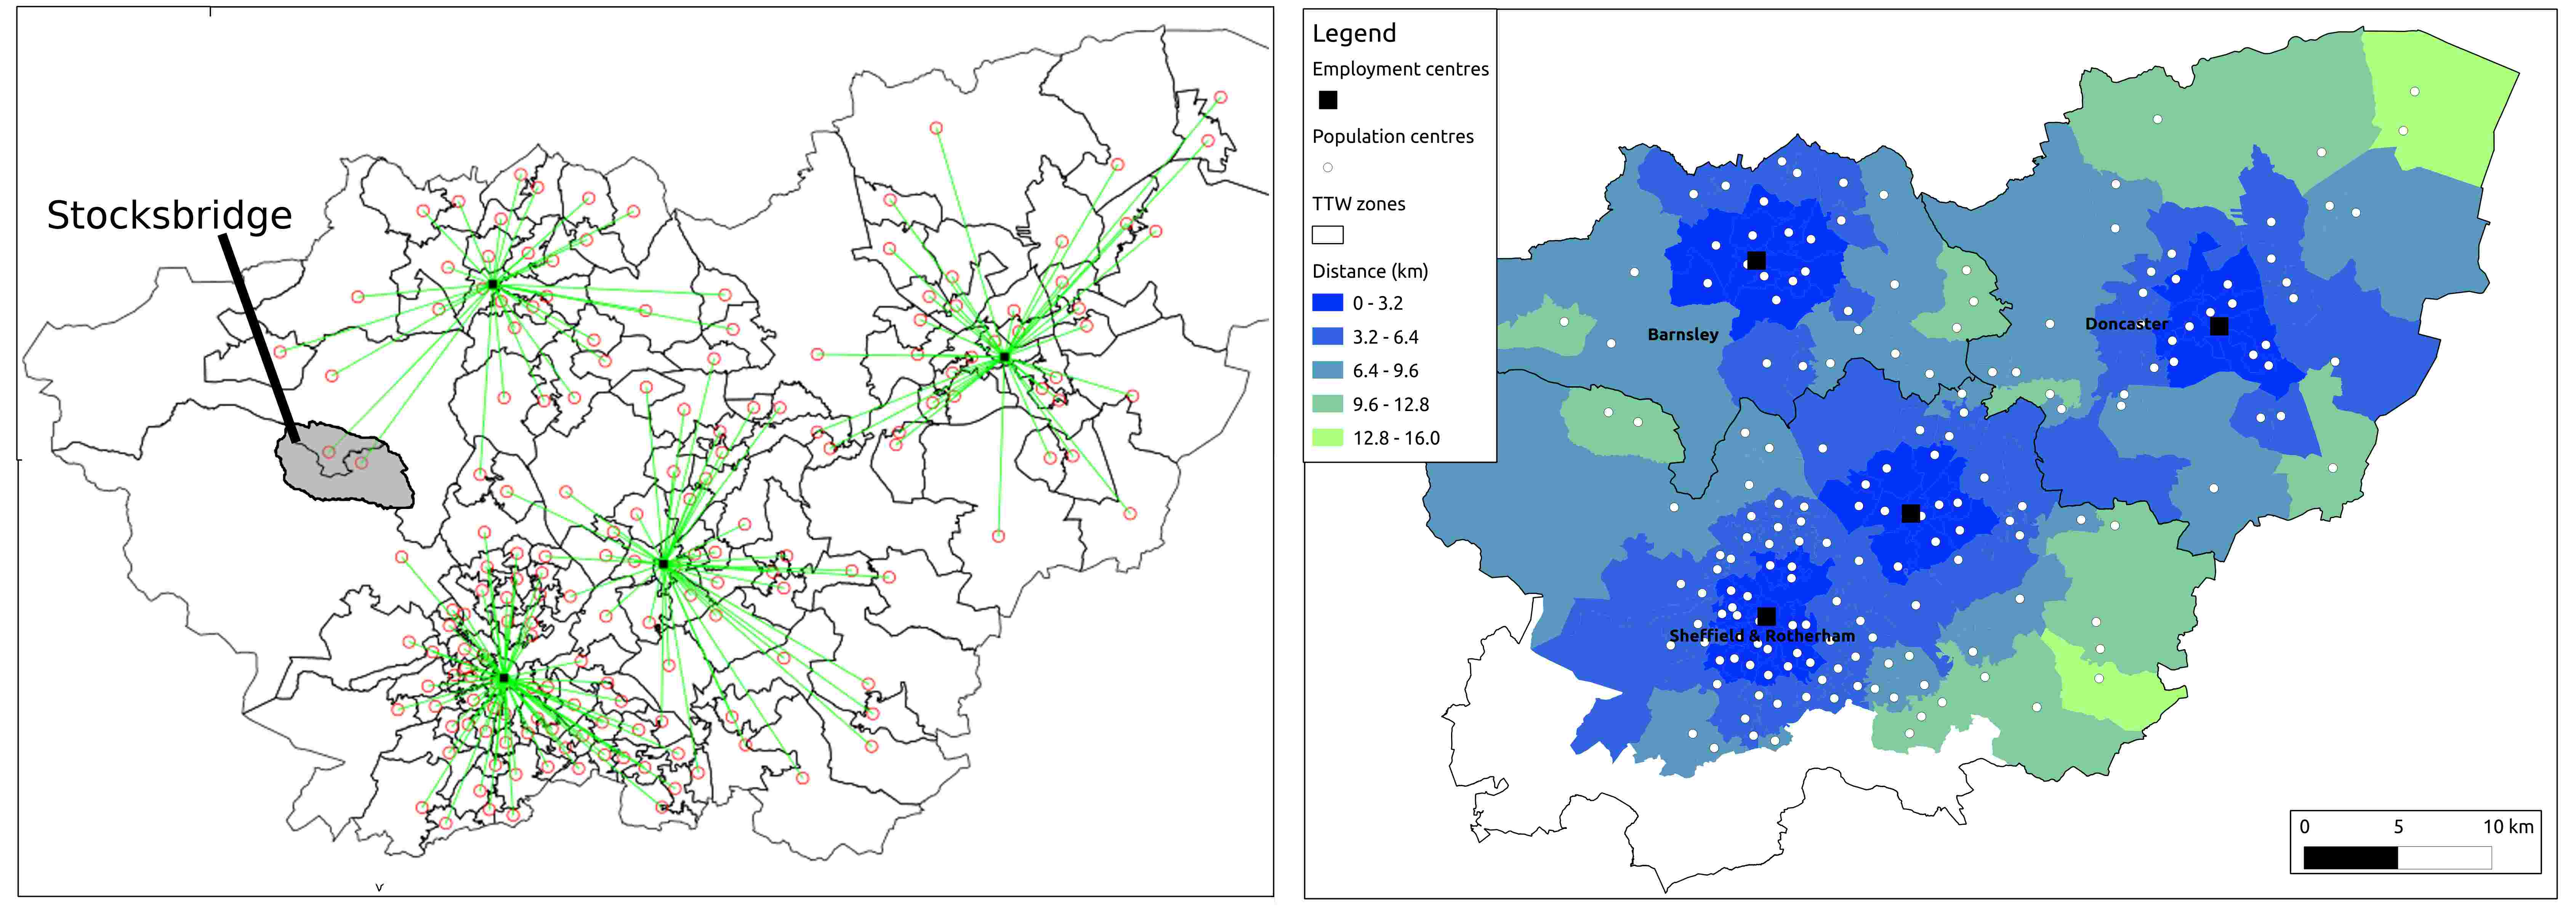
\includegraphics[width = 13 cm]{distances-msoa2}
% \end{center}
% \caption[Average distance to employment centre in South Yorkshire]{Average
% distance to employment centre in South Yorkshire. The
% left-hand map illustrates how distance was calculated (using the command
%  nncross() in the R package `spatstat'). The right-hand map illustrates
% the results --- Sheffield and Rotherham are grouped together in the same
% travel to work zone.}
% \label{fig:dis-msoa}
% \end{figure}
% 
% Rather than assuming that work centres are always located in the city
% centre, a more realistic approach is to acknowledge that a variety of
% employment centres exist, and that the relative importance of each varies from
% place to place. This is illustrated in Fig.~\ref{fig:sflow}, a flow diagram of
% the work locations of commuters based on the outskirts of Sheffield. Although
% Barnsley is the closest city centre to Stocksbridge (see
% Fig.~\ref{fig:dis-msoa}), this analysis makes it clear that Sheffield is the
% primary non-home workplace.
% 
% \begin{figure}
% \centering{
%  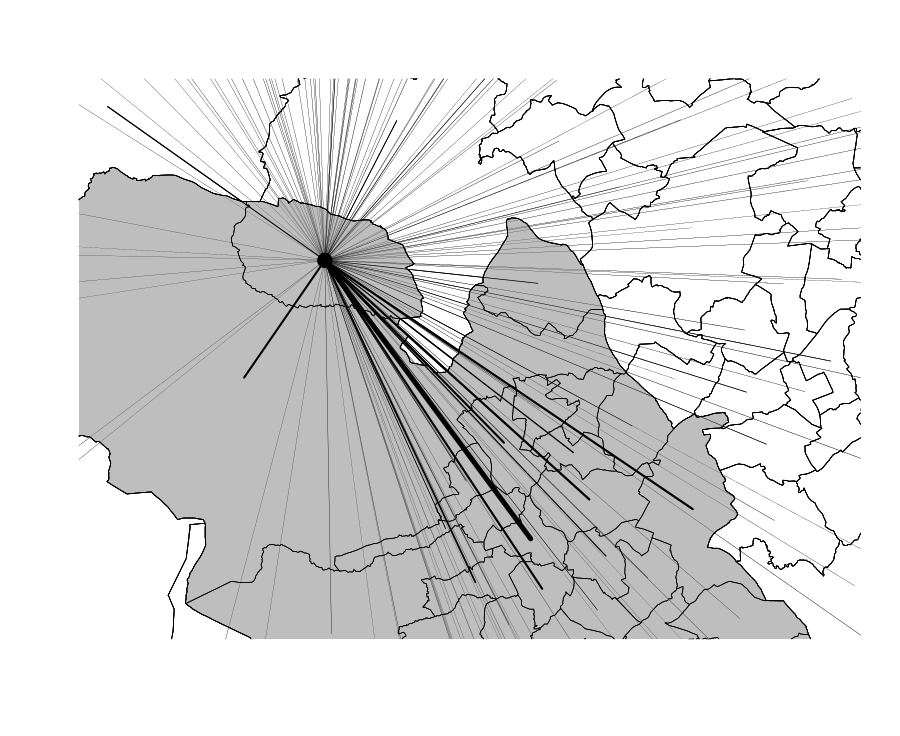
\includegraphics[width = 10 cm]{sflows}}
% \caption[Flow diagram illustrating popular commuter destinations for citizens
% of Stocksbridge]{Flow diagram illustrating popular commuter destinations for
% citizens
% of Stocksbridge. The thickness of the lines is proportional to the number of
% people who travel there (for reference, 661 people travel to
% the centre of Sheffield --- illustrated by the thickest line ---
% and 2036 people work in Stocksbridge --- illustrated by the dot
% from which all lines radiate. n = 6,338).}
% \label{fig:sflow}
% \end{figure}
% 
% The analyses presented in both Fig.~\ref{fig:dis-msoa} and Fig.~\ref{fig:sflow}
% both greatly oversimplify trip routes. The straight lines underestimate travel
% distance, completely ignoring the transport network. A more
% realistic method is to randomly allocate each individual to a unique home
% location based on
% % data on houses, and work
% % locations based on commuter flow data and the distance they travel to work
% population density (or, potentially, local area classification) and estimate
% the route taken using shortest trip algorithms dependent on the mode of
% transport used (\cref{fig:agent}). This latter method allows for the
% calculation of route distances by mode, but is more complex and difficult to
% implement over large areas.
% %\footnote{?}
% The method used to model the home-work flows presented in \cref{fig:agent},
% following the transport network, was as follows:
% \begin{itemize}
%  \item Allocate home locations to individuals in each ward. This was done
% by a stratified sample allocating individuals to smaller OA zones. Simple
% random sampling, using QGIS, created points within each zone.\footnote{This
% technique is not ideal for a couple of reasons. First, output areas do not all
% have the same working population, so it is not strictly true to say that the
% probabilities of inhabiting any of them is the same. (The mean and standard
% deviation of the working population of all 165,665 OAs in England in the 2001
% Census is 136 and 43, respectively and ranges from 0 for an area in East Dorset
% to 2121 in an area in Telford.) This problem could be easily be overcome by
% setting the number of points sampled for each OA proportional to their commuting
% population. A more severe problem for extensive OAs is that the selected points
% are unlikely to be actual houses; people could be allocated home coordinates in
% forests, mountains or even rivers as OAs provide contiguous geographical
% coverage. Methods for allocating individuals to residential building layers,
% instead of anyway, are being developed (as of December 2013) at the University
% of Southamption (Alan Smith, 2013, personal communication.)
% }
% \item Allocate a work destination for each individual. This was done by: 1)
% allocating the destination work location to concentric rings surrounding the
% ward centroid (\cref{fig:agent}); 2) randomly allocating the
% destination to a destination whose centroid lies within the allocated distance
% band, with the probability set proportional to the flow to that destination
% (from Nomis flow data); and 3) randomly selecting a point from the destination
% ward.\footnote{Work location could be allocated more precisely using the same
% technique, but harnessing the OA flow data illustrate in \cref{flows2bigemps}.}
% \item Calculating the route distance using the QGIS ``Road graph'' plugin. The
% network data for pedestrians and cars was loaded from a PostGIS database of OSM
% data; pedestrians and cyclists used the pedestrian part of the network; all
% other users used the road network.\footnote{Ideally, an automated
% batch-processing of shortest route would be used instead of the GUI of Road
% graph. This would allow more than 20 routes to be calculated. The route-planning
% Routino software was designed for use on the OSM network, so would be ideal for
% this purpose.}
% \item Save the results in an individual level variable.
% \end{itemize}
% The penultimate step in this process was the most problematic. It took a long
% time to import the OSM route network into a format that Road graph could
% understand, and each shortest route calculation took around 10 seconds (far
% longer than Google's routing service). Also, the two-way division of the
% transport network is not realistic: bicycles cannot follow all pedestrian paths
% and trains can clearly not follow roads. In addition, evidence from GPS traces
% suggests that in many cases the shortest route is not in fact the one taken
% (e.g.~\citealp{Ehrgott2012}). None of these difficulties are intractable,
% especially as the OSM transport network and software to handle it continue to
% improve.\footnote{The trip planning platform
% \href{http://opentripplanner.com/}{OpenTripPlanner} is a good example of this
% as it is rapidly developing multi-mode trip planning capabilities worldwide,
% base on the OSM and local authority data. The capability of this software can
% be tested on the \href{http://london.optitrans.net/}{Optitrans} website, a
% London-based multi-mode routing service.}
% Due to time constraints and the immaturity of some of the software used to
% batch process optimal routes, however, routing was omitted from the central
% calculation of energy costs. The impact of route choice on energy costs are
% further discussed in \cref{Chapter6}.
% 
% % \footnote{This analysis results from 20 randomly selected
% % individuals (2 of
% % whom worked at home) from the spatial microsimulation model output for
% % Stocksbridge and allocated origin-destination points based on known distance
% % bands, ward-ward commuter flows, and the population density distribution of
% % Stocksbridge.
% % }
% 
% \begin{figure}
%  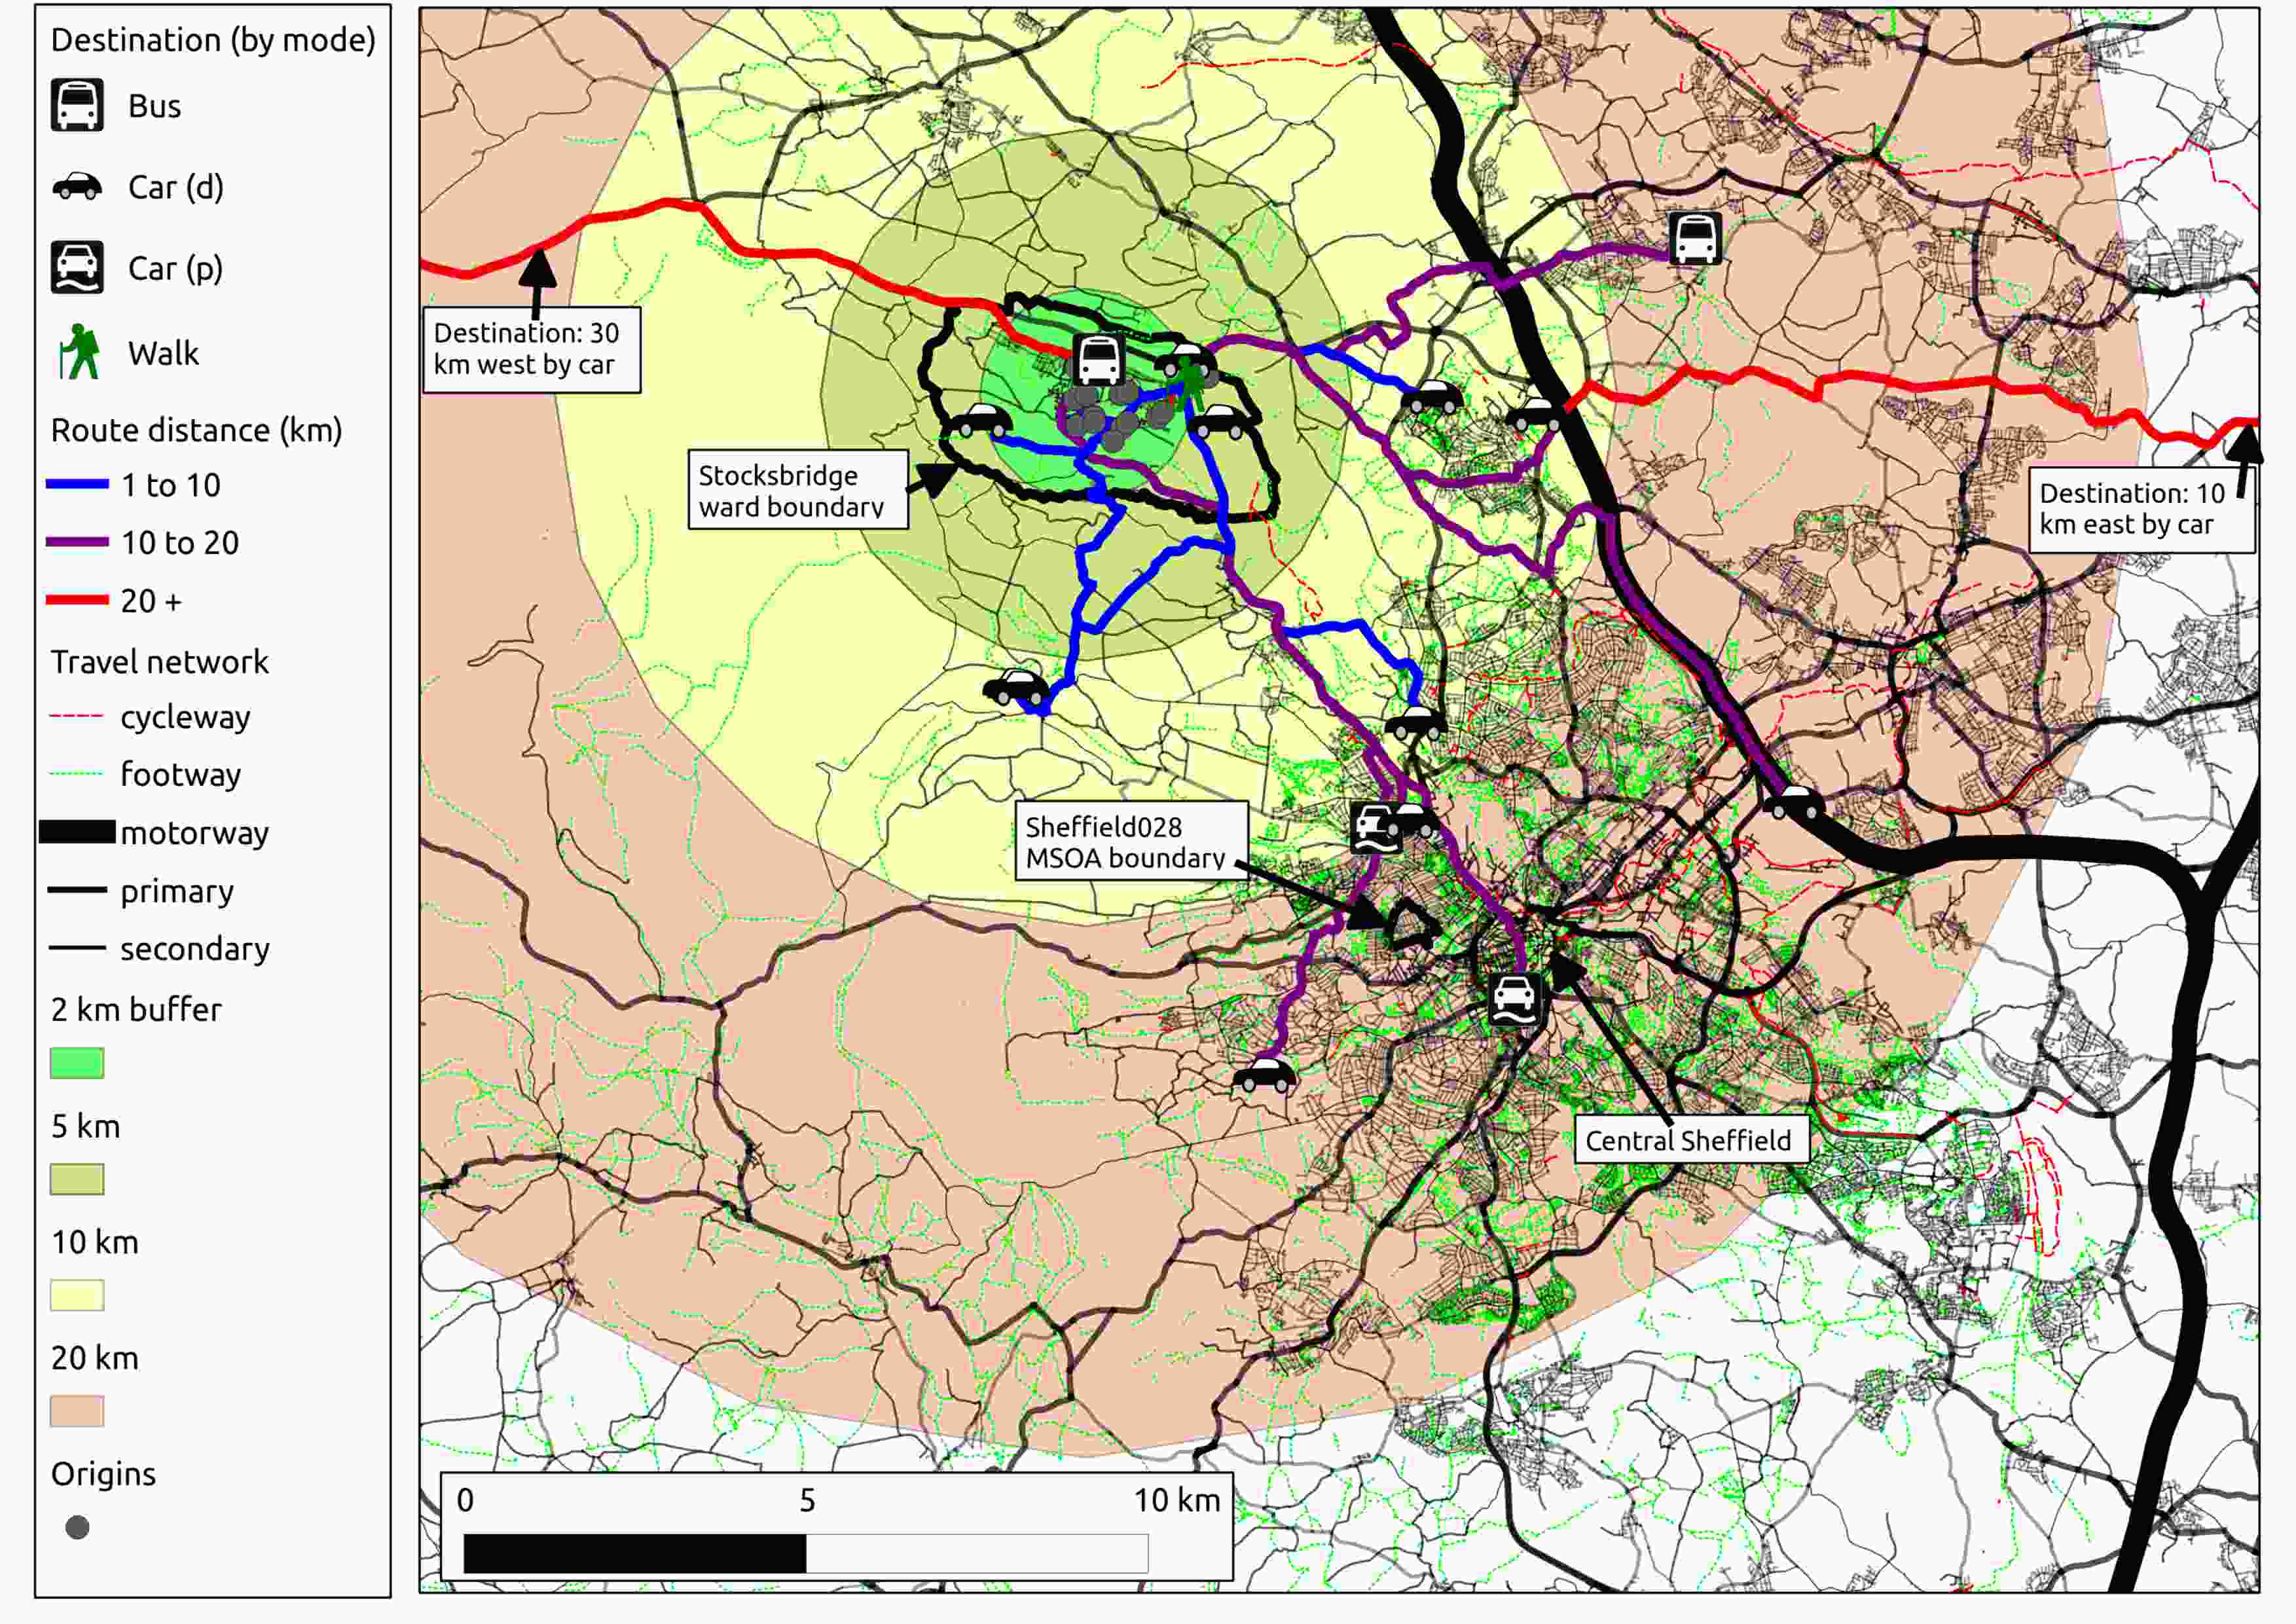
\includegraphics[width = 13 cm]{agents4}
% \caption[Simulated route choice for 20 randomly selected individuals]{Simulated
% route choice for 20 randomly selected individuals
% from the spatial simulation model. Destinations were determined by 1) subsetting
% destination wards by distance from Stocksbridge centre, 2) assigning
% probabilities of working in each ward for each distance band (based on flow
% data presented in Fig.~\ref{fig:sflow}) and 3) randomly selecting points
% within the resulting destination wards. (Workplaces of 2 people who work from
% home are not mapped).}
% \label{fig:agent}
% \end{figure}
% 
% % \subsection{Visualising flow data} % Should be in visualisation section!!!
% 
% 
